% !TEX TS-program = xelatex
% !BIB program = bibtex
% !TEX encoding = UTF-8 Unicode

\documentclass[
  twoside,
  openright,
  theme     = B,
  degree    = master,               % degree = master | doctor
  language  = chinese,              % language = chinese | english
  fontset   = template,             % fontset = default | template | system | overleaf
  watermark = true,                 % watermark = true | false
  doi       = true,                 % doi = true | false
]{ntuthesis}

 % !TeX root = ./main.tex

% --------------------------------------------------
% 資訊設定(Information Configs)
% --------------------------------------------------

\ntusetup{
  university    = {國立臺灣大學},
  university*   = {National Taiwan University},
  college       = {工學院},
  college*      = {College of Engineering},
  institute     = {工業工程學研究所},
  institute*    = {Graduate Institute of Industrial Engineering},
  title         = {整合電動車與風力電場之虛擬電廠收益分析},
  title*        = {Profit Analysis of a Virtual Power Plant Consisting of a Wind Farm and Electric Vehicles},
  author        = {彭新翔},
  author*       = {Hsin-Hsiang Peng},
  ID            = {R05546030},
  advisor       = {吳文方},
  advisor*      = {Wen-Fang Wu},
  date          = {2021-10-01},         % 若註解掉,則預設為當天
  oral-date     = {2021-10-01},         % 若註解掉,則預設為當天
  DOI           = {10.6342/NTU202103859},
  keywords      = {虛擬電廠, 風力電場, 電動車, 時間序列預測, 模型預測控制},
  keywords*     = {Virtual Power Plant, Wind Farm, Electric Vehicle, Time Series Prediction, Model Predictive Control},
}

% --------------------------------------------------
% 加載套件(Include Packages)
% --------------------------------------------------

% \usepackage[numbers]{natbib}            % 參考文獻
\usepackage[square,sort&compress,comma,numbers]{natbib}
\usepackage[normalem]{ulem}             % 下劃線、雙下劃線與波浪紋效果
\usepackage{CJKulem}
\usepackage{amsmath, amsthm, amssymb}   % 數學環境
\usepackage{commath, mathtools}         % 數學符號
\usepackage{booktabs}                   % 改善表格設置
\usepackage{multirow}                   % 合併儲存格
\usepackage{diagbox}                    % 插入表格反斜線
\usepackage{array}                      % 調整表格高度
\usepackage{longtable}                  % 支援跨頁長表格
\usepackage{paralist}                   % 列表環境

\usepackage{graphicx}                   % 插入圖片
\usepackage{float}                      % 浮動位置

\usepackage{siunitx}                    % 國際單位制度
\usepackage[version=4]{mhchem}          % 化學式
\usepackage{lscape}                     % 橫向表格
\usepackage[final]{microtype}

\usepackage{layouts}
\usepackage{threeparttable}
\usepackage{enumitem}
\usepackage{adjustbox}

\usepackage{chngcntr}                   % 腳註編號
\counterwithout{footnote}{chapter}

% --------------------------------------------------
% 套件設定(Packages Settings)
% --------------------------------------------------
% \setcitestyle{numbers}

\appendgraphicspath{{./figures/chapter01/}}
\appendgraphicspath{{./figures/chapter02/}}
\appendgraphicspath{{./figures/chapter03/}}
\appendgraphicspath{{./figures/chapter04/}}
\appendgraphicspath{{./figures/chapter05/}}
\appendgraphicspath{{./figures/chapter06/}}
\appendgraphicspath{{./figures/appendix01/}}
\appendgraphicspath{{./figures/appendix02/}}

% --------------------------------------------------
% 客制設定(Custom Settings)
% --------------------------------------------------
% 單位設置
\sisetup{group-separator = {,}}
\DeclareSIUnit{\Wh}{{\watt\hour}}           % 瓦時 Wh
\DeclareSIUnit{\TWh}{{\tera\watt\hour}}     % 百萬兆瓦時 TWh

% 數學符號
\newcommand*\diff{\mathop{}\!\mathrm{d}}
\newcommand*\Diff[1]{\mathop{}\!\mathrm{d^#1}}
\allowdisplaybreaks[1]

% 表格條列
\newcommand{\tabitem}{~~\llap{\textbullet}~~}

\raggedbottom

\begin{document}

% 封面與口試審定
% Cover and Verification Letter
\makecover                          % 論文封面(Cover)
\makeverification                   % 口試委員審定書(Verification Letter)

% 致謝與論文摘要
% Acknowledgement and Abstract
% !TeX root = ../main.tex

\begin{acknowledgement}

感谢

\end{acknowledgement}       % 致謝(Acknowledgement)
% !TeX root = ../main.tex

% 中文摘要
% Chinese Abstract
\begin{abstract}

持續成長的電力需求以及民眾環保意識抬頭,加上傳統集中式電力系統的缺點日漸浮現,各國紛紛開始關注能夠充分利用再生能源且具有良好環境效益的分散式發電(Distributed Generation, DG)技術。

本研究以虛擬電廠(Virtual Power Plant, VPP)概念整合分散式能源的風力電場與作為儲能裝置的電動汽車,考慮時間電價進行調度規劃來參與電力市場交易,並透過模型預測控制(Model Predictive Control, MPC)在有限時域下針對動態變化的虛擬電廠進行發電與儲能規劃來獲得最佳收益;其中,為鼓勵電動汽車整合於虛擬電廠中參與電力市場交易,本研究中提出以額外充電作為紅利取代直接給予金錢的鼓勵方式;此外,本研究提出了基於小波轉換對時間序列進行訊號分解,並結合傳統時間序列預測與支持向量迴歸預測的小波分解 ARIMA-SVR 組合預測模型,用以根據歷史風速資料預測風力電場發電。

並於案例模擬中使用我國\uline{東吉島}測站 2018 年間的歷史風速資料為基礎,進行短期風力預測與收益模型分析後,驗證了此最佳化收益方案的可行性。分析結果亦顯示,短期風速預測中採用小波分解 ARIMA-SVR 組合預測模型相較傳統單一預測模型在預測能力上有小幅度提升,而使用了電動汽車作為儲能裝置的虛擬電廠能夠獲取更高的收益。

\end{abstract}

% 英文摘要
% English Abstract
\begin{abstract*}

With the increasing demand for electricity and the rising of public awareness of environmental protection, as well as the increasingly emerging disadvantages of traditional centralized power system, more and more attention has been paid to distributed generation (DG) by each county, which can make full use of renewable energy and has good environmental benefits.

In this study, the concept of Virtual Power Plant (VPP) was applied to integrate with wind farms as distributed generation and electric vehicles as energy storage devices, participating in electricity market transactions by considering Time of Use Price (TOU) for scheduling. Model Predictive Control (MPC) was used to maximize benefits from power generation and storage planning for dynamic changed virtual power plants in finite time domain. Of which, in order to integrate electric vehicles into virtual power plants and participate in electricity market transactions, the compensation payment mode of providing free charging instead of direct giving of money was adopted in this study. Furthermore, the signal decomposition of time series based on wavelet transform was proposed in this study, and the traditional time series prediction and wavelet decomposition ARIMA-SVR combination prediction model for support vector regression  prediction were combined to predict wind farm power generation based on historical wind speed data.

Based on the historical wind speed data of \uline{DONGJIDAO} in 2018 in the case simulation, the feasibility of this profit optimization model was verified after applying the short-term wind power forecast and profit model. The analysis results also showed that compared with the traditional single prediction model, there is a small increase by adopting ARIMA-SVR combined prediction model with wavelet decomposition in the short-term wind power forecast. While the virtual power plant using electric vehicles as energy storage devices could obtain higher profits.

\end{abstract*}
              % 摘要(Abstract)

% 生成目錄與符號列表
% Contents of Tables and Denotation
\maketableofcontents                % 目錄(Table of Contents)
\makelistoffigures                  % 圖目錄(List of Figures)
\makelistoftables                   % 表目錄(List of Tables)
% % !TeX root = ../main.tex

\begin{denotation}[3cm]

\item[VPP]{虛擬電廠(Virtual Power Plant)}
\item[EM]{電力市場(Electric Market)}
\item[WF]{風力電場(Wind Farm)}
\item[EV]{電動汽車(Electric Vehicle)}
\item[$p_e(t)$]{時刻 $t$ 的電力價格}

\end{denotation}
            % 符號列表(Denotation)

% 論文內容
% Contents of Thesis
\mainmatter
% !TeX root = ../main.tex

\chapter{緒論}

本章為緒論,將簡述國內外電力需求狀況與傳統發電技術困境,並分別從電力系統發展、再生能源發展、電動汽車發展以及我國能源情勢等面相切入研究背景,最後說明本研究預期達到的目標以及章節組成架構。

\section{前言}

% 電力需求持續成長
能源是人類社會維持生存與文明發展所不可或缺的基礎資源,但隨著經濟發展與科技進步所延伸出的能源危機、空氣汙染與溫室效應等問題,儼然已是世界各國不得不面對的緊迫難題。長期以來,國內外的電力需求持續成長,圖 \ref{figure: Yearly Electricity Consumption in Taiwan} 為\uline{臺灣}地區年度用電數量 \cite{boe2021data},顯示自 $1999$ 年至 $2019$ 年間,\uline{臺灣}地區的年度用電數量由 $1,609$ 億度 ($160.9$ \si{\TWh}) 成長至 $2,666$ 億度 ($266.6$ \si{\TWh});於此同時,圖 \ref{figure: Yearly Electricity Consumption over World} 的世界各國年度用電數量 \cite{enerdata2020gesy} ,亦顯示世界各國的年度用電數量由 $126,050$ 億度 ($12,605$ \si{\TWh}) 成長至 $231,040$ 億度 ($23,104$ \si{\TWh}),其中又以我國在內的亞洲地區成長最為顯著。考量未來產業變遷、電動汽車普及等新增用電需求,我國經濟部預估在 $2021$ 年至 $2027$ 年間,\uline{臺灣}地區平均用電數量每年將成長約 $2.50\%$,年度用電數量將於 $2025$ 年達到 $3,091$ 億度 ($309.1$ \si{\TWh}) \cite{boe2021report}。

% 年度用電量統計數據
\begin{figure}[h]
  \centering
  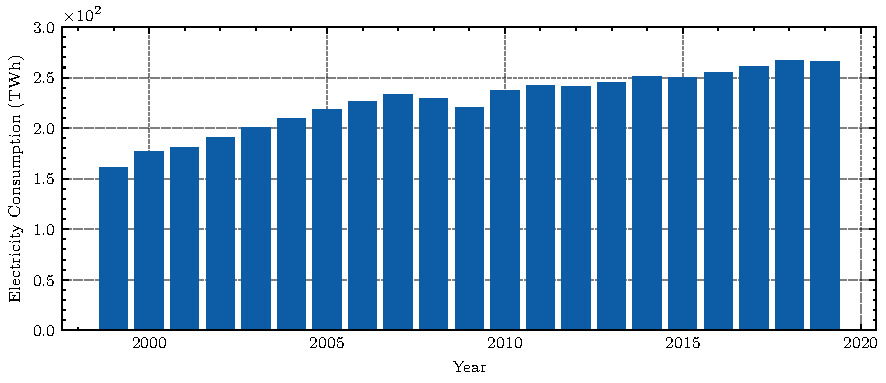
\includegraphics[width=\textwidth]{yearly-electricity-consumption-in-taiwan}
  \caption[\uline{臺灣}地區年度用電量]{\uline{臺灣}地區年度用電數量 \cite{boe2021data}}
  \label{figure: Yearly Electricity Consumption in Taiwan}
\end{figure}

\begin{figure}[h]
  \centering
  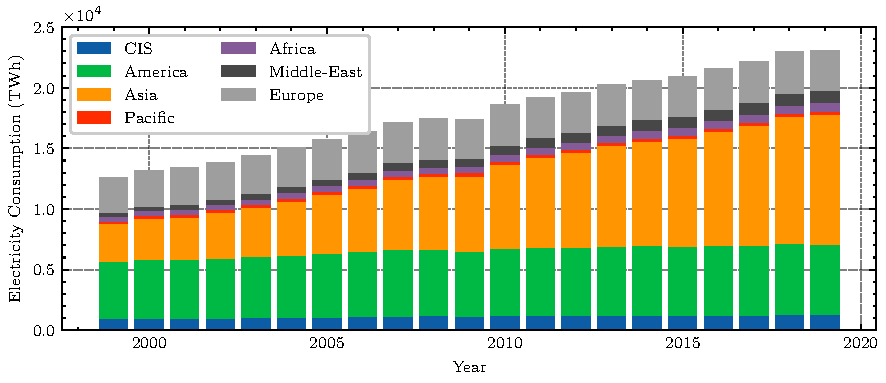
\includegraphics[width=\textwidth]{yearly-electricity-consumption-over-world}
  \caption[世界各地年度用電量]{世界各地年度用電數量 \cite{enerdata2020gesy}}
  \label{figure: Yearly Electricity Consumption over World}
\end{figure}

% 傳統發電佔比與缺點
目前世界各國的電力來源,主要以火力發電與核能發電為主,統計資料顯示,在 $2020$ 年時,火力發電與核能發電約佔全球總發電數量的 $70.92\%$ \cite{owid2020electricity},在\uline{臺灣}更佔總發電數量的 $93.40\%$ \cite{boe2021data}。其中火力發電需要大量開發燃煤、石油與天然氣等不可再生能源,也因此導致相關產業的溫室氣體排放量居高不下;而核能發電雖然有著較高的發電效率,並且幾乎沒有空氣汙染問題,但卻隱含安全隱憂,比如 $1986$ 年發生於俄羅斯的\uline{車諾比}事件 (Chernobyl disaster)、$1979$ 年發生於美國的\uline{三哩島}事件 (Three Mile Island accident) 與 $2011$ 年發生於日本的\uline{福島}第一核電廠事故 (Fukushima Daiichi nuclear disaster)。

% 虛擬電廠概念興起
民眾環保意識抬頭與核能發電安全隱憂的時空背景下,世界各國開始重新審視既有的能源產業與政策。於此同時,能夠充分利用再生能源並具有良好環境效益的分散式發電 (Distributed Generation, DG) 觀念,受到了越來越多的關注;為了降低將分散式電源併入既有電力系統所帶來的不穩定性,人們致力於發展能夠即時監控與調度分散式電源的智慧電網 (smart grid) 技術,以及可以在電網運作發生問題時即時斷開,藉此提升電力系統可靠度的微型電網 (micro grid) 技術,隨著資訊與電網技術的進步,也使虛擬電廠 (Virtual Power Plant, VPP) 概念應運而生。

\section{研究背景}

\subsection{電力系統發展}

% 電力系統定義:集中式電力系統 / 分散式電力系統
電力系統是指由發電系統、輸電系統與配電系統所組成的複雜系統,負責處理電力供給中依序會經歷的發電 (generating)、輸電 (transmission) 與配電 (distribution) 等過程 \cite{gonen2015electric}。根據電力系統中的發電系統規模,可以分為集中式電力系統 (centralized generated power system) 與分散式電力系統 (distributed generated power system)。在集中式發電系統中,電力的供給是火力、水力或核能等大型發電廠發電後,透過變電所提升電壓再經由電網輸送到用電端。而分散式電力系統,一般是由裝置容量較小的中小型發電設備所組成,分散地布置於用電端周圍 \cite{nissen2009high}。

% 臺灣供電系統架構
目前我國包含\uline{臺灣}本島、\uline{澎湖}、\uline{金門}與\uline{馬祖}在內之電力供應,由隸屬於中華民國經濟部的國營事業機構------\uline{臺灣}電力股份有限公司負責,其供電系統架構如圖 \ref{figure: Taiwan Power System Structure} 所示,圖中由火力、水力與核能發電廠產生的電力,需透過變壓器將電壓提升至超高壓 ($345$ \si{\kV}),再利用輸電線路輸送電力,然後經由超高壓變電所 ($161$ \si{\kV}) 與一次變電所 ($69$ \si{\kV})降壓後提供大型用戶用電,並透過配電變電所、二次變電所及配電系統再進行降壓,提供一般用戶使用 \cite{taipower2019supply}。

\begin{figure}[htbp]
  \centering
  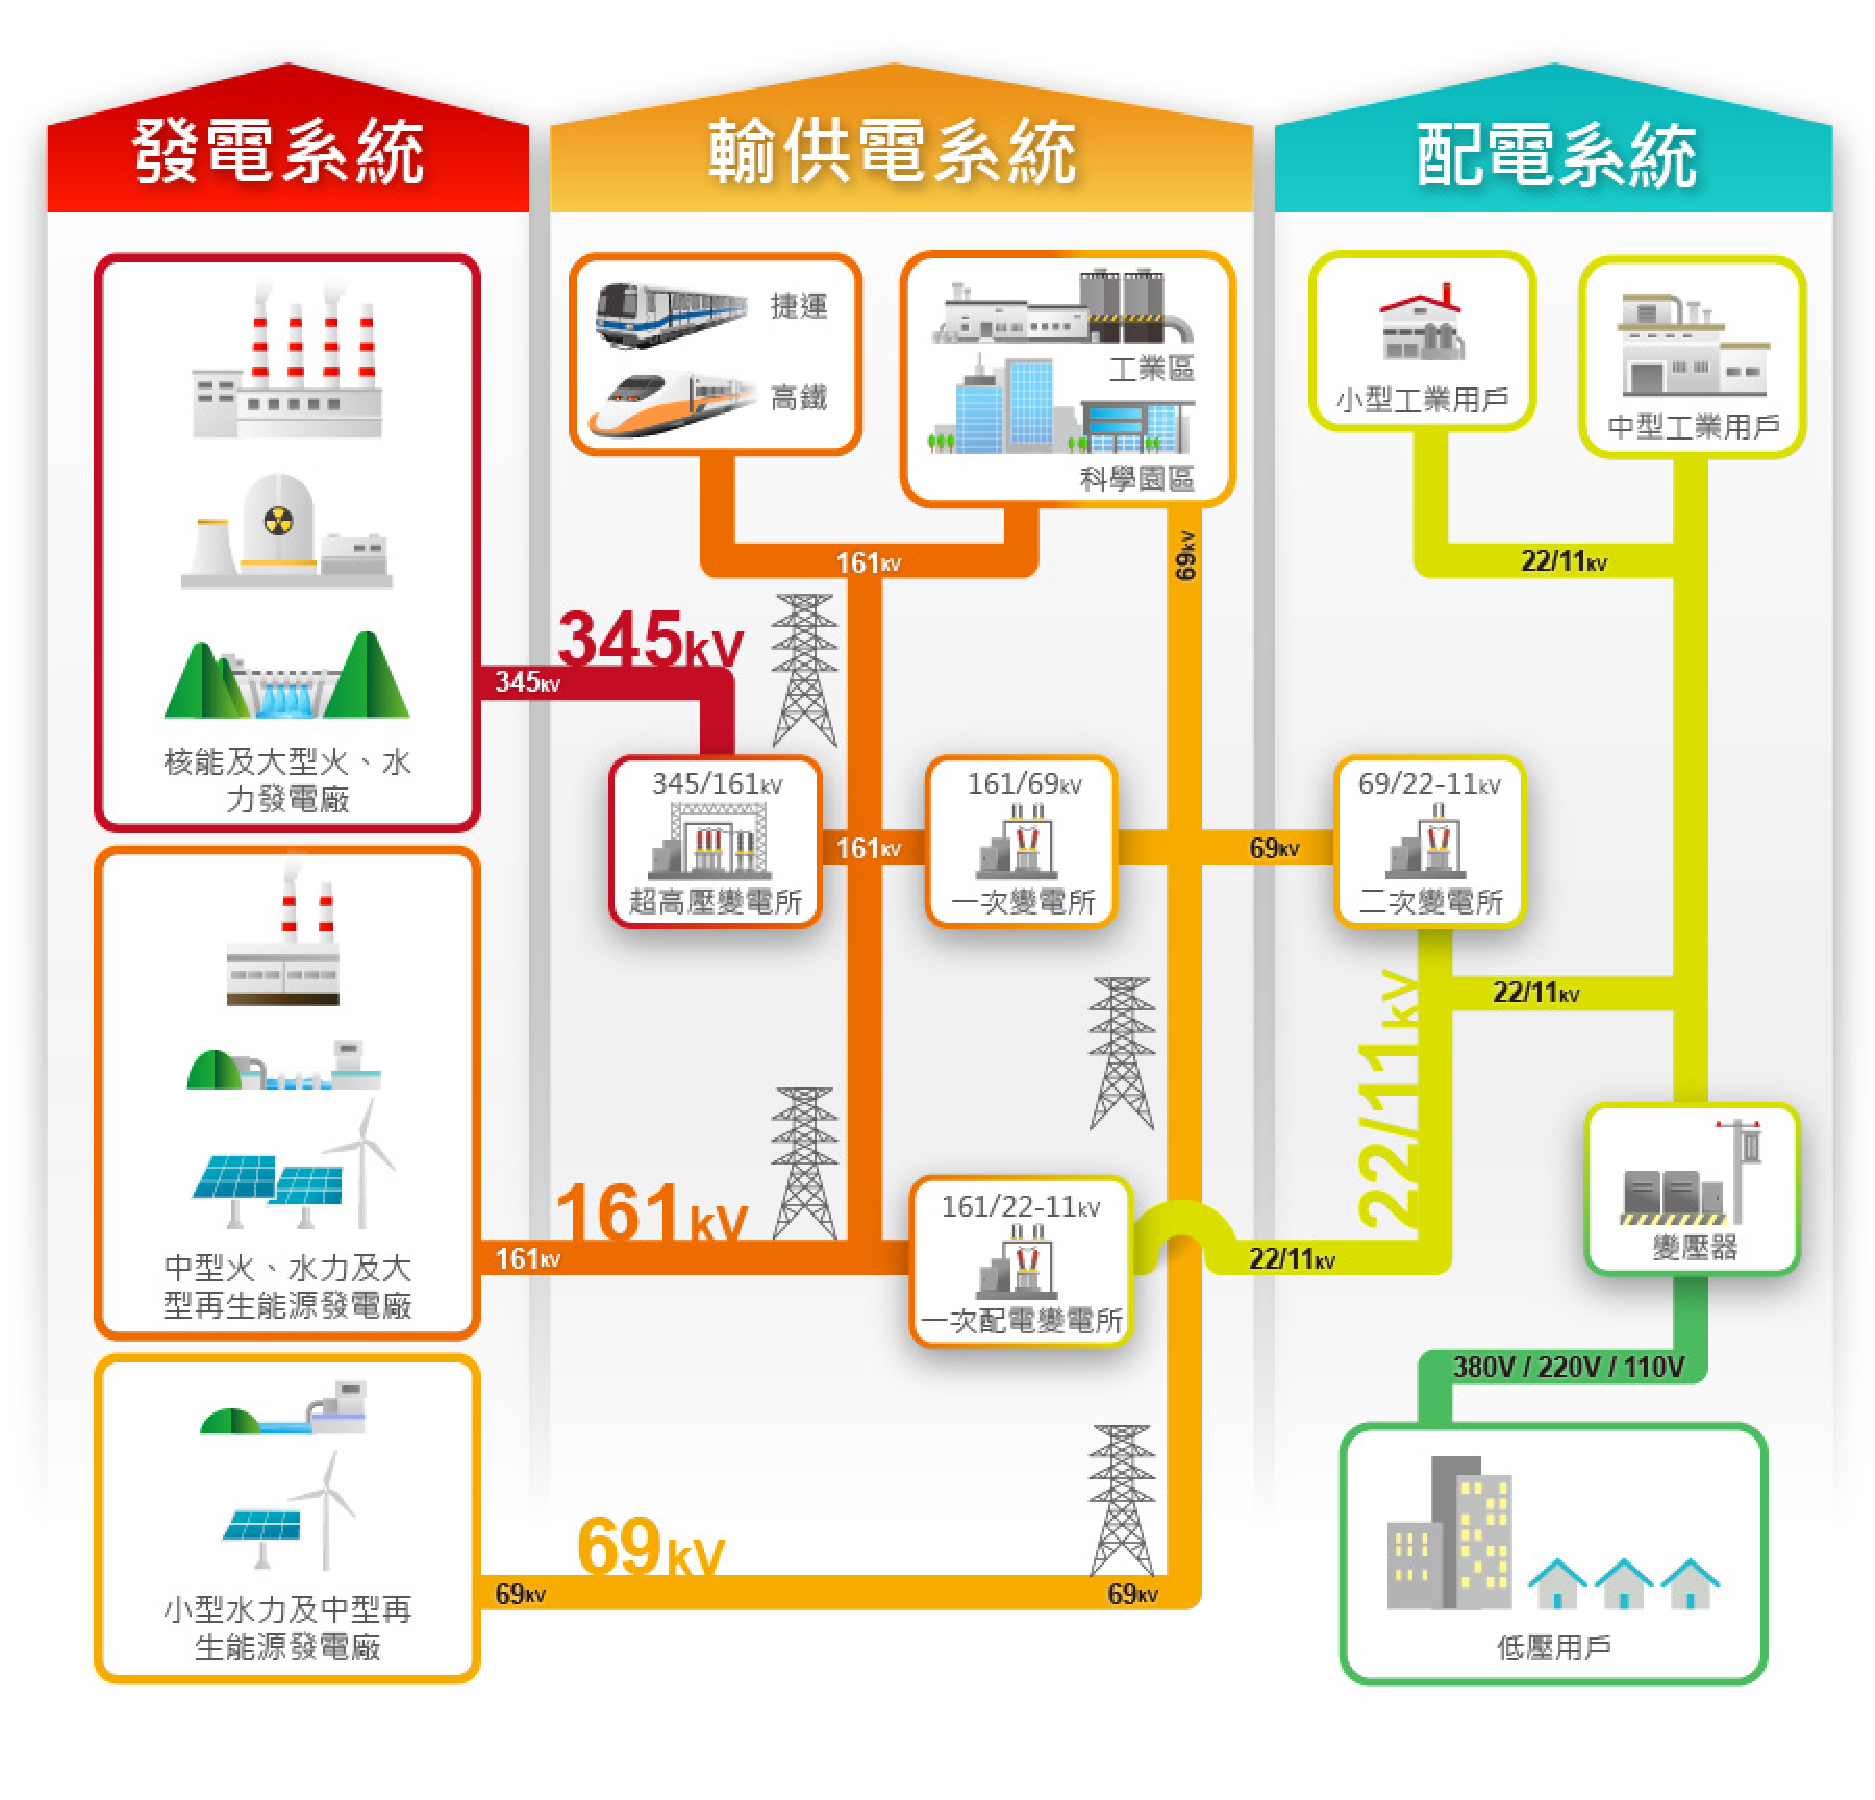
\includegraphics[width=0.75\textwidth]{Taiwan Power System Structure}
  \caption[臺灣電力股份有限公司供電系統架構]{臺灣電力股份有限公司供電系統架構 \cite{taipower2019supply}}
  \label{figure: Taiwan Power System Structure}
\end{figure}

% 傳統發電系統困境
現今世界各國的電力系統仍以傳統的集中式發電系統為主,雖然長期以來具有很好的規模經濟效益,然而隨著經濟與科技的發展,人們對於能源供給穩定性的要求日益提高,傳統集中式大型電網系統的缺陷也逐漸浮現。目前所面臨的問題,大致上可以歸納為以下幾點:

\begin{itemize}
  \item \textbf{發電機組集中建設,長距傳輸能量折損}:考量到建設成本,發電機組與用電用戶所在地通常距離遙遠,容易導致電力生產與分配不均,需要跨區輸電來解決電力不足問題,如此長距離的電力傳輸過程所累積的能量損失亦十分可觀。以\uline{臺灣}地區為例,輸電系統分為北、中、南三個地區,過往資料顯示在用電的尖峰季節,北部地區的電力仍需依靠中南部地區補足,而在過去十年間臺灣地區的電力線路損失率約為 $4\%$ \cite{boe2021data}。
  \item \textbf{局部故障影響整體,供電穩定備受考驗}:在輸配電網中,超過負載的高壓電纜將使得過載電流必須由附近的其他輸配電纜負責分攤,大量的電流回流可能導致輸配電纜超出負載而燒斷,最終故障擴散而導致大面積的停電效應。比如 $2003$ 年美加大停電、$2006$ 歐洲大停電、$2012$ 年印度大停電、$2018$ 日本\uline{北海道}大停電與 $2021$ 美國\uline{德州}大停電等大規模停電事件。
  \item \textbf{發電倚賴化石燃料,悖離能源永續目標}:燃煤、石油與天然氣等火力發電燃料屬於不可再生能源,在生產電力的過程中也伴隨著溫室氣體的排放,核能發電亦隱含安全隱憂。國際間越趨重視相關環境保護與資源永續問題,傳統集中式大型電網的主要發電方式勢必需要改善。
\end{itemize}

% 分散式發電、智慧電網、微型電網
由於上述集中式發電系統的種種問題,能夠有效利用再生能源的分散式發電系統越發受到重視,受限於裝置容量較小無法逕自取代大型電廠進行供電,分散式能源目前多採併入既有電網的形式,但再生能源本身具有的隨機性可能會阻礙電力系統的運行 \cite{guan2009research},為了儘量減少併網所引起的線路耗損與不可靠性,世界各國均致力於發展智慧電網與微型電網。智慧電網由電力系統與資訊系統所構成,藉由感測器即時監控電網系統行為,分析電力供給與需求後,再根據資訊即時調整電力系統狀態;微型電網可以視作一個小型的電力系統,整合多個中小型發電機組與電力用戶組成拓撲結構,可以透過切換連接模式或孤島模式,提升電力系統可靠度。除此之外,使用智慧電網與微型電網技術整合不同分散式能源的虛擬電廠亦受到各方重視,\uline{美國}、\uline{德國}、\uline{日本}、\uline{中國}與\uline{法國}等紛紛開始發展相關研究項目,盼能在解決電力調度與穩定運行問題的同時,打破傳統垂直壟斷的電力市場,建立競爭的市場機制。

\subsection{再生能源發展}

% 再生能源定義
再生能源 (renewable energy) 是指能夠持續不斷地從自然過程中獲取能量的資源,包括太陽能、風力、水力、地熱、生物燃料等;由於再生能源的獲得與使用過程中,所排放的汙染物相對較低,並且能降低對環境的危害性,因此又被稱作綠色能源 (green energy)。

表 \ref{table: Total 100-years CO2 Emissions from Different Energy Technologies} 為各類發電技術於生命週期內的碳排放量 \cite{jacobson2009review},使用二氧化碳當量 (carbon dioxide equivalent, CO2e) 作為測量碳足跡 (carbon footprints) 的標準單位,並以 $100$ 年排放量作為基準,資料顯示風力發電與太陽能發電的碳排放量,相較於其他發電技術都要來的少;然而再生能源所能帶來的益處遠不止於此,一份以美國\uline{加州}地區以量化工具衡量風力發電與太陽能發電的研究指出,若是提高太陽能與風力發電的裝置容量與發電數量,同時進行水資源管理,可以減少人們對於地下水的需求,進一步降低供水壓力與糧食危機 \cite{He2019}。

\begin{table}[htbp]
  \centering
  \caption[各類發電技術於生命週期內的碳排放量]{各類發電技術於生命週期內的碳排放量 \cite{jacobson2009review}}
  \begin{threeparttable}[t]
  \begin{tabular}{lccc}
    \toprule
    \textbf{能源技術} & \textbf{生命週期排放} \tnote{1} & \textbf{延遲機會成本} \tnote{2} & \textbf{人為熱量排放} \tnote{3} \\
    \midrule
    天然氣 & $179 \sim 405$ & $46 \sim 62$ & $0.61$ \\
    陸域風電 & $7.0 \sim 10.8$ & $0$ & $-1.7 \sim -0.7$ \\
    離岸風電 & $9 \sim 17$ & $0$ & $-1.7 \sim -0.7$ \\
    地熱發電 & $15.1 \sim 55.0$ & $14 \sim 21$ & 0 \\
    水力發電 & $17 \sim 22$ & $41 \sim 61$ & 0 \\
    海浪發電 & $21.7$ & $4 \sim 16$ & $0$ \\
    潮汐發電 & $10 \sim 20$ & $4 \sim 16$ & $0$ \\
    核能發電 & $9 \sim 70$ & $64 \sim 102$ & $1.6$ \\
    生物燃料 & $43 \sim 1730$ & $36 \sim 51$ & $3.4$ \\
    燃煤發電 & $230 \sim 935$ & $46 \sim 62$ & $1.5$ \\
    太陽能板 (屋頂) & $15 \sim 34$ & $-12 \sim -16$ & $-2.2$ \\
    太陽能板 (工業) & $10 \sim 29$ & $0$ & $-2.2$ \\
    聚光太陽能熱發電 & $8.5 \sim 24.3$ & $0$ & $-2.2$ \\
    \bottomrule
    & & & \hfill \si[per-mode=symbol]{\gram\text{-CO2e}\per{\kilo\watt\hour}}
  \end{tabular}
     \begin{tablenotes}
     \item[1] {\footnotesize 包括了建造、運轉與生產過程中所產生的碳排放}
     \item[2] {\footnotesize 建造與運營之間的時間延遲及壽命結束時翻新技術的額外停機時間}
     \item[3] {\footnotesize 包括燃燒或核反應釋放到空氣中的人為碳排放;太陽能發電技術透過將陽光轉換為電能來減少表面陽光,因此呈現為負值}
  \end{tablenotes}
  \end{threeparttable}%
  \label{table: Total 100-years CO2 Emissions from Different Energy Technologies}
\end{table}%

% 風機裝置容量
\begin{figure}[htbp]
  \centering
  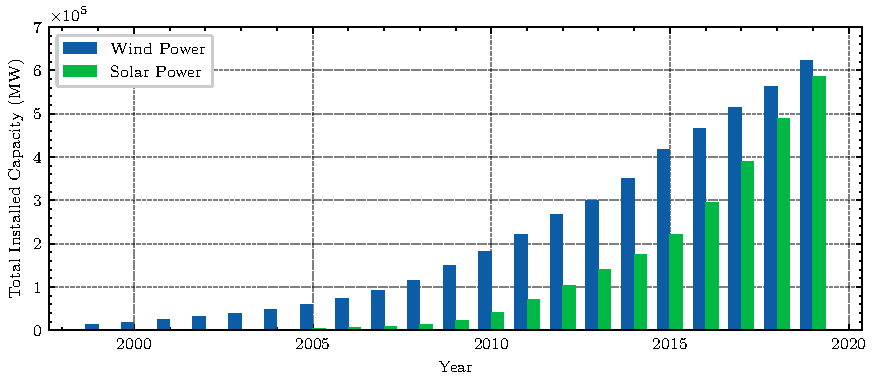
\includegraphics[width=\textwidth]{global-wind-and-solar-power-installation}
  \caption[全球風力與太陽能發電累積裝置容量]{全球風力與太陽能發電累積裝置容量 \cite{owid2020renewable}}
  \label{figure: Global Wind and Solar Power Installation}
\end{figure}

% 國際風力與太陽能發展
聯合國為了抑制持續嚴峻的全球暖化現象,於 $1997$ 年制定「\uline{京都}議定書」,規範工業國家未來的溫室氣體排放目標,各國此後逐漸將能源產業開發重心轉移至能夠減少碳足跡的核能發電與再生能源上。圖 \ref{figure: Global Wind and Solar Power Installation} 為 $1999$ 年至 $2019$ 年的全球風力發電與太陽能發電累積裝置容量 \cite{owid2020renewable},顯示全球的風力發電累計裝置容量從 $1999$ 年僅 $13,426$ 千瓩 ($13,426$ \si{\MW}),成長至 $2019$ 年的 $622,704$ 千瓩 ($622,704$ \si{\MW});而太陽能發電累計裝置容量則自 $1999$ 年僅 423 千瓩 ($423$ \si{\MW}),成長至 $2019$ 年的 $586,421$ 千瓩 ($586,421$ \si{\MW}),不難看出無論是風力發電亦或是太陽能發電皆發展迅速,足以彰顯各國落實減碳的決心

國際能源署 (International Energy Agency, IEA) 在 2021 年發布了一份關於全球如何在 2050 年達到淨零碳排的報告,說明如何在確保穩定能源供應的前提下,過渡到達成淨零碳排的目標,報告中提出了兼具成本效益與經濟生產的途徑,即是以風力發電和太陽能發電為基礎實現潔淨且有彈性的能源經濟 \cite{iea2021net}。近年來,受到招標競標與綠色憑證等市場機制影響,加上國際政策支持和建置成本降低,風力發電與太陽能發電等再生能源發展前景十分強勁,全球風能協會 (Global Wind Energy Council, GWEC) 預估到 $2024$ 年風力發電將再有約 $300,000$ 千瓩 ($300,000$ \si{\MW}) 的新增裝置容量 \cite{ohlenforst2019global},國際能源署則預估到 $2024$ 年時,太陽能發電的新增裝置容量將成長至 $600,000$ 千瓩 ($600,000$ \si{\MW}) \cite{iea2019report}。

\subsection{電動汽車發展}

% 電動汽車定義
電動車 (Electric Vehicle, EV) 是指具備單個或多個電動馬達,得以將電能轉換為動能來驅動的車輛。對於環境永續的議題而言,傳統依賴內燃機帶來動力的交通工具,在離開生產線之後,每單位里程的溫室氣體排放量就已經固定了下來;而電動汽車的溫室氣體排放量,卻能夠隨著能量來源越趨潔淨而逐年降低。近年來科技發展迅速,電動汽車電池的使用方式,除了過往由電網供電至電動汽車的 G2V (Grid to Vehicle) 模式,亦發展出了能夠反向由電動汽車輸電至電網的 V2G (Vehicle to Grid) 模式,因此電動汽車能夠在閒置或離峰時段作為電網調度的儲能設備,起到不同時段下電力資源調度的消峰填谷作用。

% 電動汽車成長
過去電動車難以普及的原因,就供給端而言,最大的問題在於生產成本居高不下;而就需求端來說,則是續航里程不高與充電方便性受限。然而隨著技術進步,不僅僅使得電動車續航里程得以提高,更使電池生產成本自 2010 年的每度電 $1,182$ 美元,下降至 $2020$ 年的每度電 $105$ 美元,生產成本已與燃油車相近。圖 \ref{figure: Global Electric Vehicles Stock} 為全球電動車累計數量,顯示在過去十年中電動汽車數量呈現穩定增長,於 2020 年時累計已超過 $1,126$ 萬輛電動汽車,預估將在 $2030$ 年成長至 $1.45 \sim 2.30$ 億輛電動汽車\footnote{此處的統計數字與預估數量包含油電混合車,但不包含兩輪或三輪的電動機車};除此之外,目前全球 $20$ 大汽車製造商中,已有 $18$ 家宣布增加電動汽車型號的製造數量,並訂定未來僅販售電動汽車的計畫 \cite{iea2021ev}。

% 風機裝置容量
\begin{figure}[htbp]
  \centering
  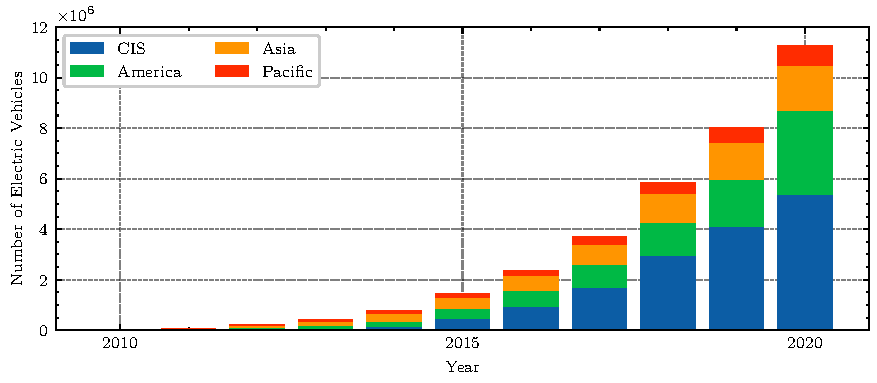
\includegraphics[width=\textwidth]{global-electric-vehicles-stock}
  \caption[全球電動車累計數量]{全球電動車累計數量 \cite{iea2021ev}}
  \label{figure: Global Electric Vehicles Stock}
\end{figure}

% 空氣汙染 -> 再生能源發展
值得一提的是,聯合國國際資源委員會 (International Resource Panel) 在 2016 年的產業報告指出,在燃煤佔比超過七成的國家推動電動汽車發展,會導致空氣汙染增加 \cite{hertwich2016green},而在 2019 年一份針對中國不同省份,了解電動車碳足跡在區域間變異性的研究,亦發現在燃煤發電佔有率較高的山東、河北等北方省份,電動汽車的碳足跡相較於燃煤汽車要來的高 \cite{wu2019assessing}。因此,單獨發展電動汽車並不能夠一勞永逸解決環境議題,如果未能同時提高綠色能源佔比,甚至可能會造成負面效果,隨著世界各國電動汽車產業的蓬勃發展,推動再生能源的進程更是刻不容緩。

\subsection{我國能源情勢}

\uline{臺灣}再生能源發展與我國政府為了因應「\uline{京都}議定書」所規範的溫室氣體減量標準有關,行政院於 1998 年召開的第一次全國能源會議,提出了以減碳為主要目標,鼓勵發展再生能源技術,首度將溫室氣體減量目標納入政策中。在 2008 年,行政院通過了《永續能源政策綱領》與《再生能源發展條例》,期望藉由政策規劃來改變能源架構,並將有限資源作有效的使用,兼顧能源安全、經濟發展與環境保護,以滿足未來世代發展的需要;在 2012  年,我國將智慧電網列入「國家節能減碳總計畫」中,致力於推動智慧電網技術,並實際推展至澎湖縣\uline{東吉島}、屏東縣\uline{林邊鄉}等處進行實域驗證;在 2015 年,通過了《溫室氣體減量及管理法》,明定國家溫室氣體長期減量目標,期望在 2050 年將溫室氣體排放量降低至 2005 年的 $50\%$ 以下。

% 臺灣政府雖在 2021 年 4 月 22 日世界地球日表態「支持 2050 淨零未來」,然而目前僅計劃在 2030 年減少 20% 碳排放,再生能源更只佔電力結構的 5.6%,發展龜步。邀請您加入推動改變的力量,透過分享文章訊息、支持能源轉型、要求政府制定足以對抗氣候危機的政策、加速發展再生能源,為您我與下一代打造一個永續、宜居、免於極端氣候威脅的地球家園。

% 我國為減少空氣汙染,行政院於 $2017$ 年通過的《空氣w汙染防制行動方案》中將分三階段推動全台電動車化,目標於 $2040$ 年達到新售汽機車全面自動化。近年來在政府補貼政策激勵下,電動汽機車逐漸受到民眾認可與青睞,電動汽機車佔新增汽機車掛牌數量逐年上升。

% 千架海陸風力機 / 陽光屋頂百萬座
為落實\uline{臺灣}環境永續,我國經濟部於 2012 年,針對風力發電與太陽能發電推動相關計畫,規劃於 2030 年達成「陽光屋頂百萬座 、千架海陸風力機」兩項願景。考量國際趨勢與民意聲浪,我國於 2016 年政黨輪替後,加速興建第三座天然氣接收站,擬定在 2025 年全面廢除核能發電並降低燃煤發電比例,達成「非核家園」的目標;為推度臺灣產業轉型,我國政府亦於 2018 年提出包含「綠能科技」產業在內的 $5+2$ 產業創新計畫,積極推動「太陽光電兩年推動計畫」、「綠能屋頂全民參與」、「風力發電四年推動計畫」、「智慧電表示範建置」、「沙崙智慧綠能科學城」等計畫,希望結合國內需求發展相關能源產業,引進國內外投資的同時增加國內需求與就業機會。為了補足廢除核能發所出現的能源缺口,立法院於 2019 年通過《再生能源發展條例》修正案,更加積極推動再生能源發展,設立 2025 年達成再生能源發電數量佔總發電數量 $20\%$ 的目標。

表 \ref{table: Renewable Energy Device Ratio in Taiwan} 為 2008 年《再生能源發展條例》通過後,我國再生能源裝置容量與發電數量之狀況 \cite{boe2021data},顯示我國再生能源發展步調雖穩健但緩慢,以此成長趨勢要在 $2025$ 年達到再生能源發電數量佔比 $20\%$ 的目標,尚有好幾許哩路要走。

\begin{table}[htp]
  \centering
  \caption[臺灣地區再生能源裝置容量與發電數量]{臺灣地區再生能源裝置容量與發電數量 \cite{boe2021data}}
  \begin{tabular}{crrrr}
    \toprule
    \textbf{年度} & \textbf{裝置容量} & \textbf{裝置容量佔比} & \textbf{發電數量} & \textbf{發電數量佔比} \\
                  & (\si{\MW})        & (\%)                  & (\si{GWh})        & (\%)                  \\
    \midrule
    $2019$        & $7,795$           & $13.9$ \%             & $15,360$          & $5.6$ \%              \\
    $2018$        & $6,246$           & $11.9$ \%             & $12,634$          & $4.6$ \%              \\
    $2017$        & $5,259$           & $10.7$ \%             & $12,390$          & $4.6$ \%              \\
    $2016$        & $4,726$           & $ 9.5$ \%             & $12,753$          & $4.8$ \%              \\
    $2015$        & $4,330$           & $ 8.9$ \%             & $10,501$          & $4.1$ \%              \\
    $2014$        & $4,065$           & $ 8.4$ \%             & $ 9,944$          & $3.8$ \%              \\
    $2013$        & $3,816$           & $ 7.8$ \%             & $10,864$          & $4.3$ \%              \\
    $2012$        & $3,594$           & $ 7.4$ \%             & $10,684$          & $4.3$ \%              \\
    $2011$        & $3,399$           & $ 7.0$ \%             & $ 8,995$          & $3.6$ \%              \\
    $2010$        & $3,197$           & $ 6.5$ \%             & $ 8,642$          & $3.5$ \%              \\
    $2009$        & $3,030$           & $ 6.3$ \%             & $ 7,808$          & $3.4$ \%              \\
    \bottomrule
  \end{tabular}
  \label{table: Renewable Energy Device Ratio in Taiwan}
\end{table}

除此之外,我國行政院於 2017 年完成《電業法》修正,開放再生能源自由交易,未來\uline{臺灣}的電力市場將採躉購制度與自由市場雙軌運作,落實電業自由化 (electricity liberalization) 以推動我國綠色產業發展;負責營運電力交易平台的電力交易中心於 2021 年 7 月 1 日揭牌啟用,劃下我國電力產業轉型的重要里程碑,平台首先推出有別於直接購買電力資源的「日前輔助服務市場」的交易制度,鼓勵民間將分散式電力資源投入平台參與電力市場交易以維持電網穩定。

% 為了由根本解決傳統大型電網所衍生出的種種問題,並邁向永續能源發展之最終目標, 智慧電網與微電網的建設、再生能源的開發以及政府政策的訂定均為不可忽略的發展方向。 因此,除了仰賴科技發展與設備的進步外,本研究希望能藉由區域性能源供需數據與電網 配電控制策略的整合提高能源使用效率,並透過電力系統設備規劃建立階段性任務,以確 保電力系統能逐步朝能源永續的目標邁進。

% 目前,無論是在確保能源穩定供應、發展潔淨能源或是提高能源使用效率等方面,均 有許多不同領域的學者致力於相關的研究,但並沒有一套有系統的方法將各研究方向進行 整合;此外,充分利用自然資源的再生能源發電方式雖然永續,但不同的自然資源會因為 地域的不同而有不同特性,再加上自然現象的變動常導致電力無法穩定供應與預測。因此, 一個完善的永續能源發展策略需要依照各地區不同的自然資源與環境特性進行規劃,以達到整體電力系統之階段性目標,引領電力系統朝能源永續邁進。

% 綜合以上,我國發展再生能源是十分可行的,但目前尚在推廣階段,而政府 所規劃、未來預計建置的裝置容量僅為期望,要實際實踐還須政府積極推廣並提 高民間參與意願。此外,以客觀學術方式檢視目前政府所規劃的再生能源發展目 標能否順利達成亦是重要議題之一,因此本研究擬應用時間序列分析方法,根據 我國歷年裝置容量數據及目前所規劃之發電能源裝置容量來建立火力及汽電共生 裝置容量預測模型,並利用預測結果配合不同達成率的「千架海陸風力機」、「陽 光屋頂百萬座」及「地面型 PV 系統可用地」等計畫作情境分析模擬,檢視我國政 府規劃 2025 年再生能源目標能否順利完成與非核家園的可能,以及對用電需求與 環境的影響。

% 電力市場自由化

\section{研究動機}

\uline{臺灣}地區地狹人稠,能源高度仰賴進口,未來核能電廠陸續除役後所造成的電力缺口,不論對民生或是經濟發展,都是一個迫切需要解決的問題。在國際情勢與民意傾向下,額外增設火力電廠必然不是首要選項,而智慧電網與微型電網的發展,讓虛擬電廠概念得以落地應用,加上電力市場自由化的到來,吸引系統營運商投資並且採用虛擬電廠,或許是一個可以嘗試的辦法。

在蒐集文獻的過程中,發現國內關於虛擬電廠的相關研究並不多,並且大多以商業模式分析為主,尚缺少一套客觀評估虛擬電廠收益的工具。考慮我國目前風力發電與太陽光電的累計裝置容量差異不大,且風力發電在相近容量裝置下,比起太陽光電具有更高的發電效率,加上國內外電動汽車產業成長趨勢顯著,本研究希望能結合風力發電與電動汽車,以車輛對電網 (Vehicle-to-Grid, V2G) 概念為基礎,構建虛擬電廠收益模型,並根據不同時段下的時間電價調度電力供需來最佳化虛擬電廠收益,以供電廠業者作為收益評估及決策之參考。

\section{研究目的}

綜合上述研究背景與研究動機,本文的研究目的條列如下:

\begin{enumerate}[label = (\arabic*), itemsep=4pt, parsep=4pt, topsep=0pt, partopsep=0pt]
  \item 了解虛擬電廠概念,整理建構收益模型所需的資料與流程;
  \item 依據資料蒐集結果,建構一套整合風力電場與電動汽車的虛擬電廠收益模型;
  \item 針對收益模型建構過程中的困難與不足之處,提出方法、進行改善;
  \item 透過案例分析,探討在不同假設情境下虛擬電廠之收益狀況。
\end{enumerate}

本文旨在建構一套分析流程,用以計算虛擬電廠中在整合風力電場與電動汽車下的收益,期望能對今後相關政策與投資評估有所助益。

% 本文擬採用虛擬電廠概念整合近年來成長趨勢顯著的電動汽車作為機動性儲能設備,使再生能源得以透過能量儲存緩衝本身的隨機性與間歇性,以短期風速預測電量為基礎,建構虛擬電廠參與電力市場的收益分析模型,並使用模型預測控制方法 (Model Predictive Control, MPC) 在有限時域內根據過去狀態進行即時性調度,期望能對今後評估虛擬電廠收益有所助益。

\section{本文架構}

本文共分六章,整體架構如圖 \ref{figure: Thesis Organization} 所示。各章內容分述如下:第一章為緒論,針對論文研究背景、研究動機與研究目的進行說明;第二章為文獻回顧,介紹本文研究內容所涉及的領域,並將蒐集到的國內外相關文獻進行統整與探討;第三章為研究方法,簡述研究流程及方法原理,做為日後驗證結果有效性的基礎;第四章為模型建構,說明本文依據前提文獻及研究方法所建構的收益模型及其建構方式;第五章為案例分析,示範分析過程並探討不同假設情境下的虛擬電廠收益狀況;第六章為結論與建議,依本研究所得到結果進行總結,最後補充說明研究限制並對未來可行的研究方向提出建議。

% [Figure] 論文架構
\begin{figure}[htbp]
  \centering
  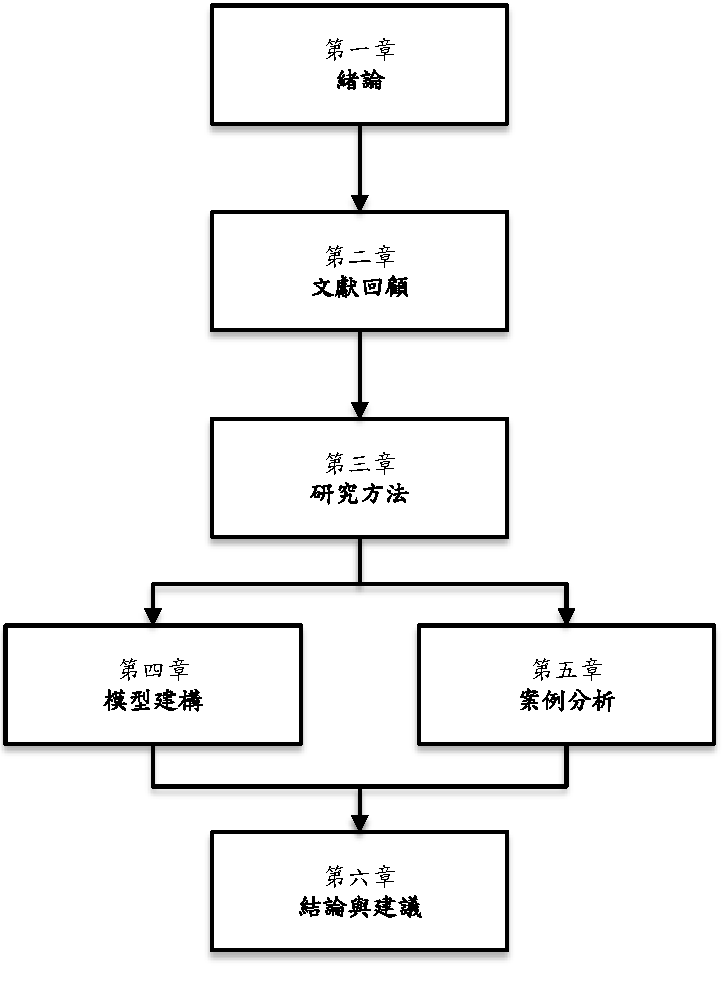
\includegraphics{thesis-organization}
  \caption[論文架構]{論文架構}
  \label{figure: Thesis Organization}
\end{figure}
% !TeX root = ../main.tex

\chapter{文獻回顧}

本章為文獻回顧,在對整合風力發電與電動汽車的虛擬電廠參與電力市場交易收益模型的建構與分析之前,需要對相關領域進行了解。以下將研究過程中蒐集的文獻經整理後分為虛擬電廠概念和風電預測評估部分進行陳述。

\section{虛擬電廠概念}

由於再生能源的間歇性與隨機性會導致電力供給與需求兩側失衡,學者們提出了整合分散式能源 (Distributed Energy Resources, DERs)、儲能設備 (Battery Energy Storage System, BESS) 與電動汽車 (Electric Vehicle, EV) 的虛擬電廠 (Virtual Power Plant, VPP) 概念。

目前學術上並未對虛擬電廠有統一的定義:在 \cite{Asmus2010} 中指稱虛擬電廠為依賴於資訊系統,透過網路通訊技術遠端控制電力系統,實現自動輸配電、需量反應與能量儲存等行為的整合網路;在 \cite{Pudjianto2007, Pudjianto2017} 中將虛擬電廠分為技術與市場兩大部分,技術層面為提供電力來源的分散式發電,市場層面進行電力市場的交易與管理;而 \cite{braun2008review} 則將虛擬電廠定義分為控制與通訊兩大單位,前者以直接集中控制方式整合分散式能源,後者透過資通訊系統整合主動用電用戶網路。

綜合上述文獻,虛擬電廠可以視為是一個具備調度發電設備、整合用戶需求的中央控制中心,其概念如圖 \ref{figure: Virtual Power Plant} 所示。其中發電設備可以包括火力發電和核能發電等傳統發電技術,也可以包括風力發電、太陽能發電等再生能源發電技術;透過資訊設備進行發電數量預測、電力價格預測、電力需求預測等,並進行需量反應管理需求與調度電力資源。

\begin{figure}[htbp]
  \centering
  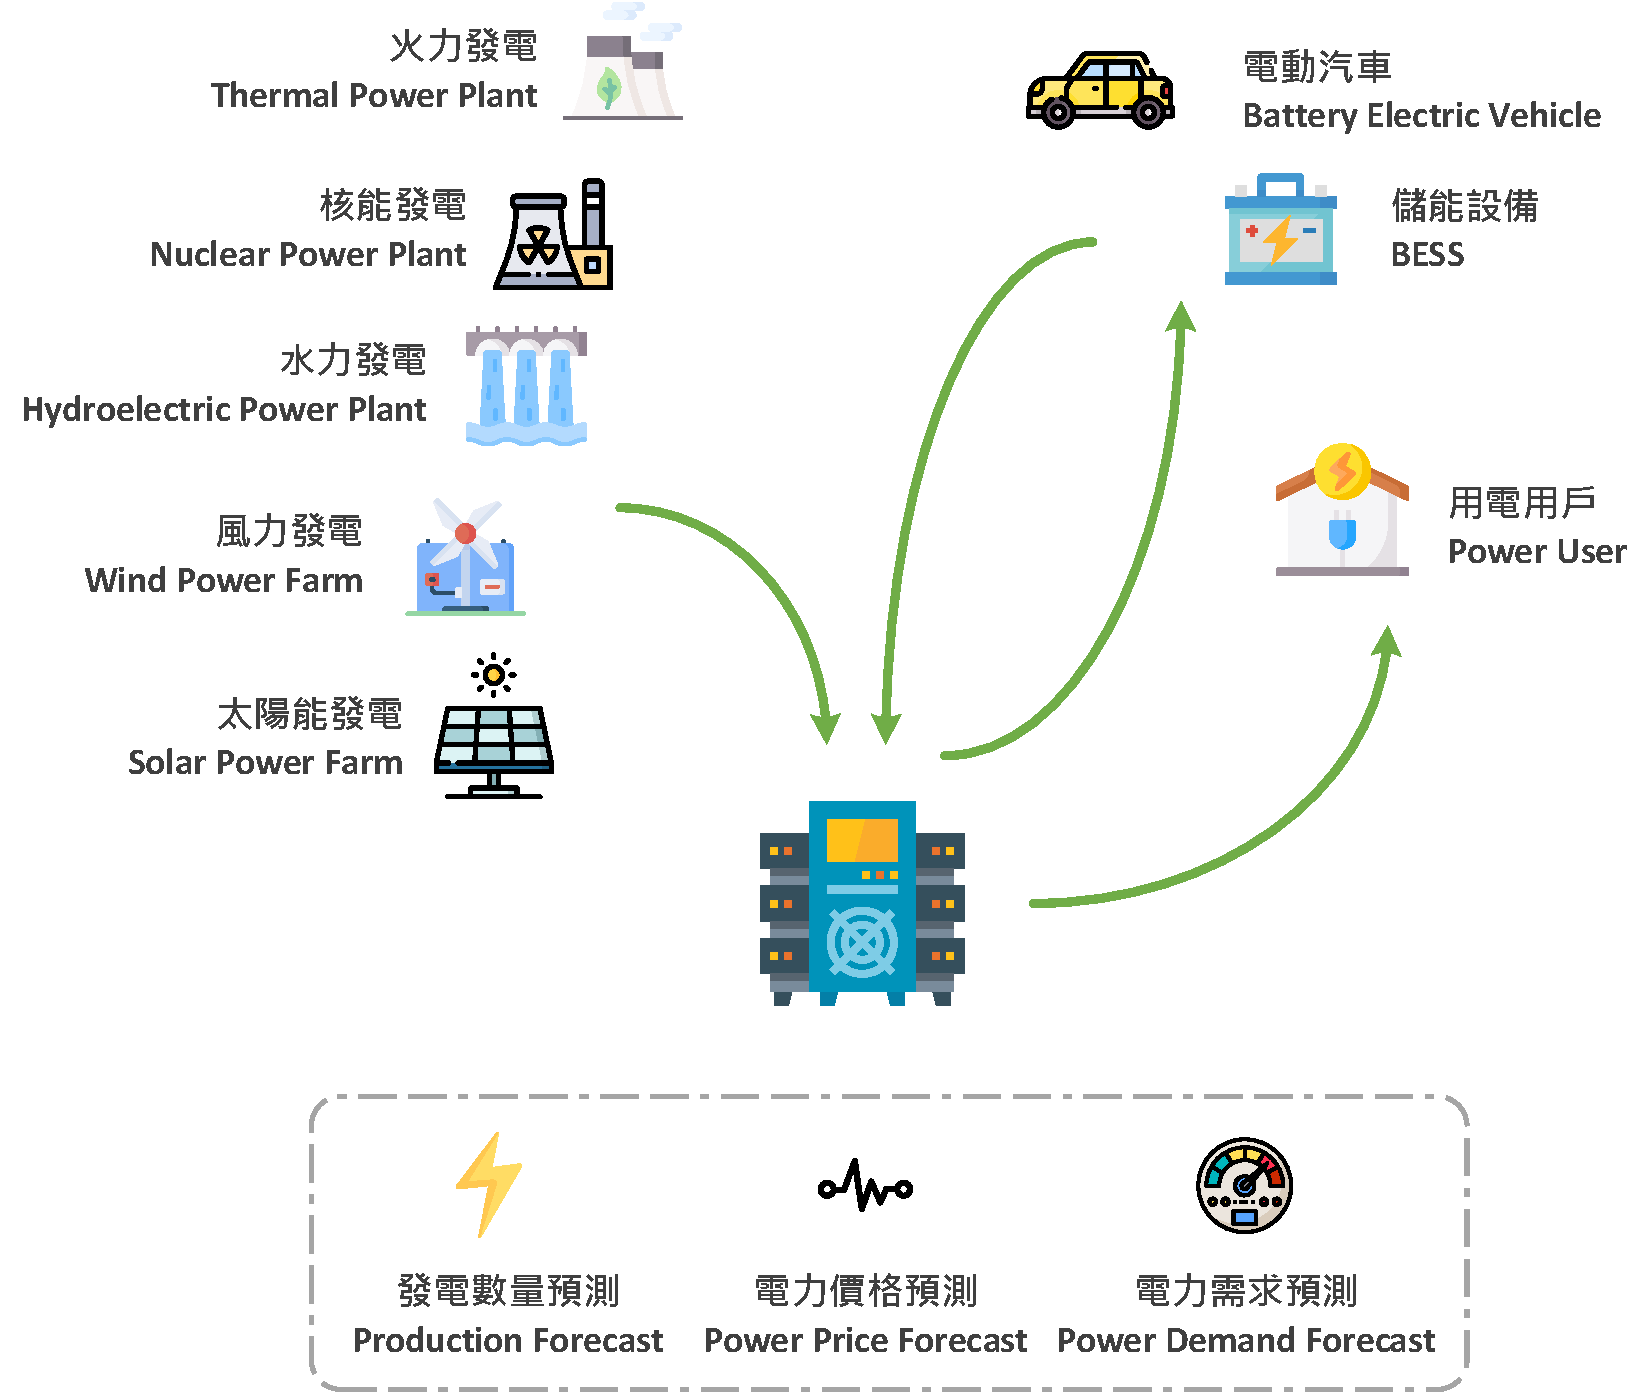
\includegraphics[width=\textwidth]{Virtual Power Plant}
  \caption{虛擬電廠概念}
  \label{figure: Virtual Power Plant}
\end{figure}

目前我國針對虛擬電廠概念進行應用與研究的相關文獻並不多,其中 \cite{U0001-2906201000281800} 應用虛擬電廠之概念探討我國電力消費型態改變是否可以減少電力使用所造成的環境衝擊,採用了生命週期評估方法量化涵蓋人體毒性、水體優養化與全球暖化等在內的八類環境衝擊項目,發現應用虛擬電廠策略後造成的電力消費型態改變可以減少因電力消費所造成之環境衝擊;\cite{U0027-0212201417510382} 提出虛擬電廠在自由電力市場中的獲利模型並分析其獲利關鍵因素,利用 IEEE 37 母線測試饋線進行最佳電力潮流 (Optimal Power Flow) 模擬,發現變壓器供電上限和儲能電池設備為虛擬電廠營運商獲利的關鍵因素;\cite{U0027-2501201611000959} 應用虛擬電廠概念整合太陽光電與電池儲能設備,並採用時間電價與需量反應概念,探討不同用戶負載情境下虛擬電廠的調度狀況,發現儲能設備的調度與時間電價有關且用戶類型不會影響儲能設備調度結果;\cite{chung2016vpp} 考慮表燈用戶、高壓用戶與整體社會參與虛擬電場運作時的經濟效益與機會成本,透過量化經濟效益模型評估不同用戶群體參與虛擬電廠是否具備經濟可行性,依據實證分析結果發現鼓勵電力用戶參與彈性電價方案有助於節省容量成本並具減碳效益,並提出政府應扶植虛擬電廠產業在我國發展、未來整體電力系統政策應具備跨系統配套方案等政策論點。

\section{風電預測評估}

風力發電是目前再生能源發電中相對成熟的技術,如何對風速與風能進行預測與評估是風力發電項目可行性研究與輸配電網規劃研究的重要工作之一。依據歷年風速與風向資料進行的風力發電效益評估,根據時間尺度與應用層面的不同,可以分為長期風能評估 (Wind Resource Assessment) 與短期風能預測 (Wind Energy Forecasting),長期風能評估用來評估一個地區是否有足夠潛力發展風力發電;而短期風能預測則用於電力系統中的調度規劃。

長期風能評估方面,多以一般統計方法將歷史風速資料與機率分布函數進行擬和,並透過風力機組的功率曲線轉換成對應的風能分布,用以評估潛在風能。目前已有許多學者投入相關研究,其中最早由 \cite{justus1976nationwide} 提出透過不同的機率密度函數描述風速,評估潛在風能的方法;\cite{nigim2007heuristic, panda1990stochastic, kumar2019wind} 採用機率分布函數擬合風速,分別評估\uline{加拿大}和\uline{印度}不同地區的潛在風能,作為風場選址考量;\cite{chuang2001wind} 分別就臺灣地區過往四十年間的平時風速與極值風速探討其適用機率分布,發現韋伯機率函數可用於描述平時風速,與 \cite{teyabeen2015statistical} 針對利比亞地區所進行的統計分析結果一致。

短期風能預測方面,目前多採時間序列方法觀察過去風速數據中隱含的趨勢,並針對風力電場進行風能預測,建立模型以預測未來風速。傳統時間序列預測的模型建構方法,根據平穩性條件可以分為應用於平穩時間序列的自迴歸模型 (Auto Regressive Model, AR Model)、移動平均模型 (Moving Average Model, MA Model) 與自迴歸移動平均模型 (Auto Regressive Moving Average Model, ARMA Model),以及應用於非平穩時間序列的差分自迴歸移動平均模型 (Auto Regressive Integrated Moving Average Model, ARIMA Model);近年來也有不少研究致力於將機器學習方法中的人工神經網路 (Artificial Neural Network, ANN) 與支持向量迴歸 (Support Vector Regression, SVR) 應用於時間序列預測。此外,為了更加準確地分析非平穩時間序列,通常會使用以下方法將時間序列進行分解:

\begin{itemize}
  \item \textbf{趨勢分解 (Trend Decomposition)} :依據季節性將時間序列模型分解為週期分量 (seasonal component)、趨勢分量 (trend component) 與殘留分量 (remainder component),再與實際數據進行擬合求解模型參數,即 STL 分解 (Seasonal-Trend Decomposition Based on LOESS) \cite{cleveland1990stl}。
  \item \textbf{訊號分解 (Signal Decomposition)}:將時間序列透過訊號處理方式分解為高頻訊號與低頻訊號,分別進行模型擬合後將預測值進行疊合。常見訊號分解方法有傅立葉轉換 (Fourier Transform, FT)、小波轉換 (Wavelet Transform, WT) 與經驗模態分解 (Empirical Mode Decomposition, EMD) 等 \cite{foster1996wavelets}。
\end{itemize}

相關研究中,\cite{liu2012comparison} 提出 ARIMA-ANN 模型與 ARIMA-Kalman 模型來預測短期風速,比較後顯示兩者皆均具有良好的性能可以用於非固定風速預測;\cite{kusiak2009short} 採用機器學習方法中的支持向量迴歸模型 (SVR Model)、多層感知器模型 (MLP Model) 與決策樹模型進行預測並比較其準確性,其中以支持向量迴歸模型的誤差最小;\cite{hu2013hybrid} 提出結合 EEMD 與 SVM 的組合模型進行風速預測,並以中國西北部的\uline{酒泉}地區數據進行驗證,發現相較於傳統時間序列預測方法具有更高的準確性;\cite{liu2013forecasting} 以小波轉換為基礎提出 Wavelet Packet-BFGS 模型、Wavelet Packet-ARIMA-BFGS
模型與 Wavelet-BFGS 模型進行短期風速預測,實驗案例表明三種混合模型都有不錯的表現;\cite{ting2015windpredict} 以\uline{梧棲}地區 2013 年的觀測資料,採用 ARIMA 模型與 LSSVM 模型進行風速預測,發現僅使用風速時間序列作為預測的結果相較於納入其餘氣象資料的多屬性時間序列預測結果更為準確。

\section{電力調度規劃}

風力發電本身具備不確定性,因此針對風力發電的電力調度最佳化模型中,通常會採用隨機動態規劃、模糊理論約束與機率分佈等方法將不確定性問題轉換為一定機率下的確定性問題,這些研究中的調度模型通常會以經濟性、環保性或可靠度作為最佳化目標。隨著數學模型的差異,所適用的最佳化方法亦十分廣泛,主要可以分為傳統數值最佳化方法與人工智慧技術最佳化方法,比如遺傳演算法 (Genetic Algorithm, GA)、模擬退火法 (Simulated Annealing, SA) 與粒子群最佳化 (Particle Swarm Optimization, PSO) 等;由於電力調度需要根據實時的資訊不斷地對前一時段的方案進行修正,此一特性與預測控制理論十分貼合,國內外亦有研究提出了在電力調度中應用模型預測控制方法 (Model Predictive Control, MPC) 進行調度最佳化求解。

比如 \cite{2011patrinos} 將電力價格與需求視為隨機過程,使用隨機模型預測控制方法,求解使營運與交易成本最低的電力調度策略;\cite{2015renaudineau} 使用粒子群最佳化方法,求解太陽能發電裝置在不同環境條件下欲維持最大輸出的追蹤問題;\cite{zhang2014application} 使用模型預測控制法結合動態規劃方法,調度電動汽車充電站的能源效益,分析不同地區下建置充電站、不同電池容量大小等因素對充電站調度的影響。

\section{小結}

目前國內外有許多優秀的學者在進行虛擬電廠相關的研究,然而我國目前仍未有針對虛擬電廠結合風力電場與電動汽車進行收益分析之相關研究。本研究旨在針對整合風力電場與電動汽車的虛擬電廠,建立收益最佳化模型並透過模型預測控制方法,針對動態變化之虛擬電廠進行規劃求解,以提供投資與可行性上的評估。

% !TeX root = ../main.tex

\chapter{研究方法}

本章為研究方法,首先對本文的研究流程進行概述,並將研究流程劃分成數據資料蒐集、風力發電預測與收益模型分析…等步驟,這一章節主要將針對各步驟中所使用到的不同的原理與方法進行介紹與說明,其餘模型建構與實現的細節則留待後續章節中提到時再進行詳細敘述。

\section{研究流程概述}

本文研究流程大致上可以劃分成數據資料蒐集、風力發電預測與收益模型分析三個步驟。數據資料蒐集部分,收集我國再生能源發電廠址資料與對應地區鄰近的中央氣象局歷史風速,作為後續風力預測以及模擬算例的依據;風力發電預測部分,主要目的在推估風力發電於各時刻的發電量,提供收益最佳化模型進行求解;收益模型分析部分,根據預測所得的各時刻風力機組預測發電數量,進行有限移動時域下的模型預測控制規劃求解。

\section{風力發電預測}

風力發電預測部分將過去風速資料透過時間序列建構風速預測模型,用以推估未來某一時刻 $t$ 的風速 $v(t)$,並根據風力機組模型轉換為對應的發電功率 $p_{wt}(t)$。其中使用的時間序列混合預測模型,是先透過小波轉換將時間序列進行分解,並分別將分解後的高頻與低頻訊號建立整合自迴歸移動平均模型與支持向量迴歸模型,最後再將預測結果進行重構。

\subsection{小波時頻分析}

短期風速預測的時間跨度較小,通常不考慮季節性影響,本研究中的時間序列分解將採用訊號處理中經常使用的小波轉換(Wavelet Transform, WT)作為處理工具,其概念與傅立葉轉換(Fourier Transform, FT)類似,目前被廣泛用於量子力學、醫學影像與機器診斷…等領域。

\subsubsection{傅立葉轉換(Fourier Transform, FT)}

標準的傅立葉轉換將訊號由時間頻域轉換至空間頻域,假設 $x(t)$ 是滿足可積分條件的時間訊號,使用 $e^{-i \omega t}$ 的弦波訊號進行組成,則其傅立葉轉換的積分表示式如方程式 \eqref{equation: Fourier Transform} 所示。

\begin{equation}\label{equation: Fourier Transform}
  \mathcal{FT}\{ x \} (\omega) = \int_{-\infty}^{\infty} x(t) e^{-i \omega t} \, \diff t
\end{equation}

由於捨棄了時間頻域的資訊,因此無法從上述傅立葉變換中得到該訊號於不同時間點的頻率資訊,例如訊號發出時間、訊號是否延遲、訊號延遲時間…等。針對傅立葉轉換無法傳達時間變化頻率的缺陷,學者 Gabor 在文獻 \cite{mallat1989theory} 中提出添加窗函數(window function)的短時傅立葉轉換(Short-Time Fourier Transform, STFT)進行分析。使用 $\omega(t - \tau)$ 作為窗函數的短時傅立葉轉換積分式如方程式 \eqref{equation: Short-Time Fourier Transform} 所示。

\begin{equation}\label{equation: Short-Time Fourier Transform}
  \mathcal{STFT}\{ x \} (\omega, \tau) = \int_{-\infty}^{\infty} x(t) \omega(t - \tau) e^{-i \omega t} \, \diff t
\end{equation}

採用不同寬度的窗函數會在時間頻域與空間頻域上有不同的解析度:較寬的窗函數有較高的空間頻域解析度,但時間頻域解析度較低;較窄的窗函數有較高的時間頻域解析度,但空間頻域解析度較低。小波轉換的積分表示式如方程式 \eqref{equation: Wavelet Transform} 所示,使用了一組具有震盪特性且能夠迅速衰減至零的小波母函數(Mother Wavelet)逼近目標函數,以解決短時傅立葉轉換中的窗函數由於大小和形狀固定,在應對不同頻率訊號時的侷限性。

\begin{equation}\label{equation: Wavelet Transform}
  \mathcal{WT}\{ x \} (a, b) = \int_{-\infty}^{\infty} x(t) \psi_{a, b}(t)
\end{equation}

其中,$\psi_{a,b} (t)$ 是作為轉換基底的小波母函數。如方程式 \eqref{equation: Mother Wavelet} 所示,式中尺度參數 $a$ 表示週期長度,平移參數 $b$ 表示移動長度,分別代表空間軸上的縮放與時間軸上的平移,滿足 $a, b \in \mathbb{R}$ 且 $a \neq 0$。

\begin{equation}\label{equation: Mother Wavelet}
   \psi_{a, b}(t) = \frac{1}{\sqrt{\abs{a}}} \psi \left( \frac{t-b}{a} \right)
\end{equation}

為滿足小波分解在不同領域應用下的需求差異,學者提出了眾多的小波母函數如 Daubechies 小波、Symlet 小波與 Coiflet 小波…等。在選擇小波母函數時會考慮以下性質:

\begin{itemize}
  \item \textbf{緊支撐(Compactly Supported)}:當尺度函數與小波函數只在有限區間內存在非零狀態,稱其具備緊支撐性,區間寬度越大的小波函數具備較好的局部分辨與去除雜訊能力。
  \item \textbf{正交性(Orthonormal)}:若小波係數之間的相關程度越小,分解後的訊號在重構後可以獲得較為平滑的效果。
  \item \textbf{對稱性(Symmetric)}:影響小波基底在變換前後的偏題程度,採用具備對稱性的小波函數分解訊號,有利於訊號的恢復與重建。
  \item \textbf{消失矩(Vanishing Moments)}:若 $\displaystyle \int \psi(t) t^m \, dt = 0$ 則稱該小波函數具有 $m$ 階的消失矩,較高的消失矩具有較好的訊號壓縮與提取資訊能力。
\end{itemize}

常見的小波母函數型態與特性如表 \ref{table: Wavelet Mother Function} 所示。

\begin{table}[htp]
  \centering
  \caption[常見小波母函數特徵]{常見小波母函數特徵}
  \begin{tabular*}{0.85\textwidth}{lccccc}
    \toprule
    \textbf{小波母函數} & \textbf{緊支撐} & \textbf{支撐寬度} & \textbf{對稱性} & \textbf{正交性} & \textbf{消失矩} \\
    \midrule
    Sinc & 否 & 無限 & 是 & 是 & 否 \\
    Harr & 是 & $1$ & 是 & 是 & $1$ \\
    Meyer & 否 & 無限 & 是 & 是 & 無限 \\
    Ricker & 否 & 無限 & 是 & 否 & $1$ \\
    Morlet & 否 & 無限 & 是 & 否 & \\
    Symlet (symN) & 是 & $2N-1$ & 近似對稱 & 是 & $N$ \\
    Coiflet (cN) & 是 & $6N-1$ & 近似對稱 & 是 & $2N$ \\
    Daubechies (dbN) & 是 & $2N-1$ & 是 & 是 & $N$ \\
    \bottomrule
  \end{tabular*}
  \label{table: Wavelet Mother Function}
\end{table}

\subsubsection{連續小波轉換(Continuous Wavelet Transform, CWT)}

小波轉換中,小波母函數的取值範圍主要依賴於尺度參數和平移參數,若 $a$ 和 $b$ 在實數域中為連續,則連續小波轉換可以表示如方程式 \eqref{equation: Continuous Wavelet Transform} 所示。

\begin{equation}\label{equation: Continuous Wavelet Transform}
  \mathcal{CWT}\{ x \} (a, b) = \frac{1}{\sqrt{\abs{a}}} \int_{-\infty}^{\infty} x(t) \bar{\psi} \left( \frac{t - b}{a} \right) \, \diff t
\end{equation}

其中,$\bar{\psi}$ 為 $\psi$ 的共軛複數。在實際情況中,小波轉換應存在其反轉換才有意義,因此必須滿足方程式 \eqref{equation: Admissible Condition} 所表示的小波轉換容許性條件(Admissible Condition),式中的 $C_{\psi}$ 稱為容許性常數(Admissible Constant),表示如方程式 \eqref{equation: Admissible Constant} 所示。

\begin{equation}\label{equation: Admissible Condition}
  0 < C_{\psi} < \infty
\end{equation}

\begin{equation}\label{equation: Admissible Constant}
  C_{\psi} = \int_{-\infty}^{\infty} \frac{\abs{\hat{\psi} (\omega)}^2}{|\omega|} \diff \omega
\end{equation}

\subsubsection{離散小波轉換(Discrete Wavelet Transform, DWT)}

離散小波變換經常被用於數值分析與時頻分析中,但並沒有簡單而明確的方程式用以表達輸入與輸出之間的關係,通常以圖 \ref{figure: Descrete Wavelet Transform} 所示的階層式架構表示。

\begin{figure}[htbp]
  \centering
  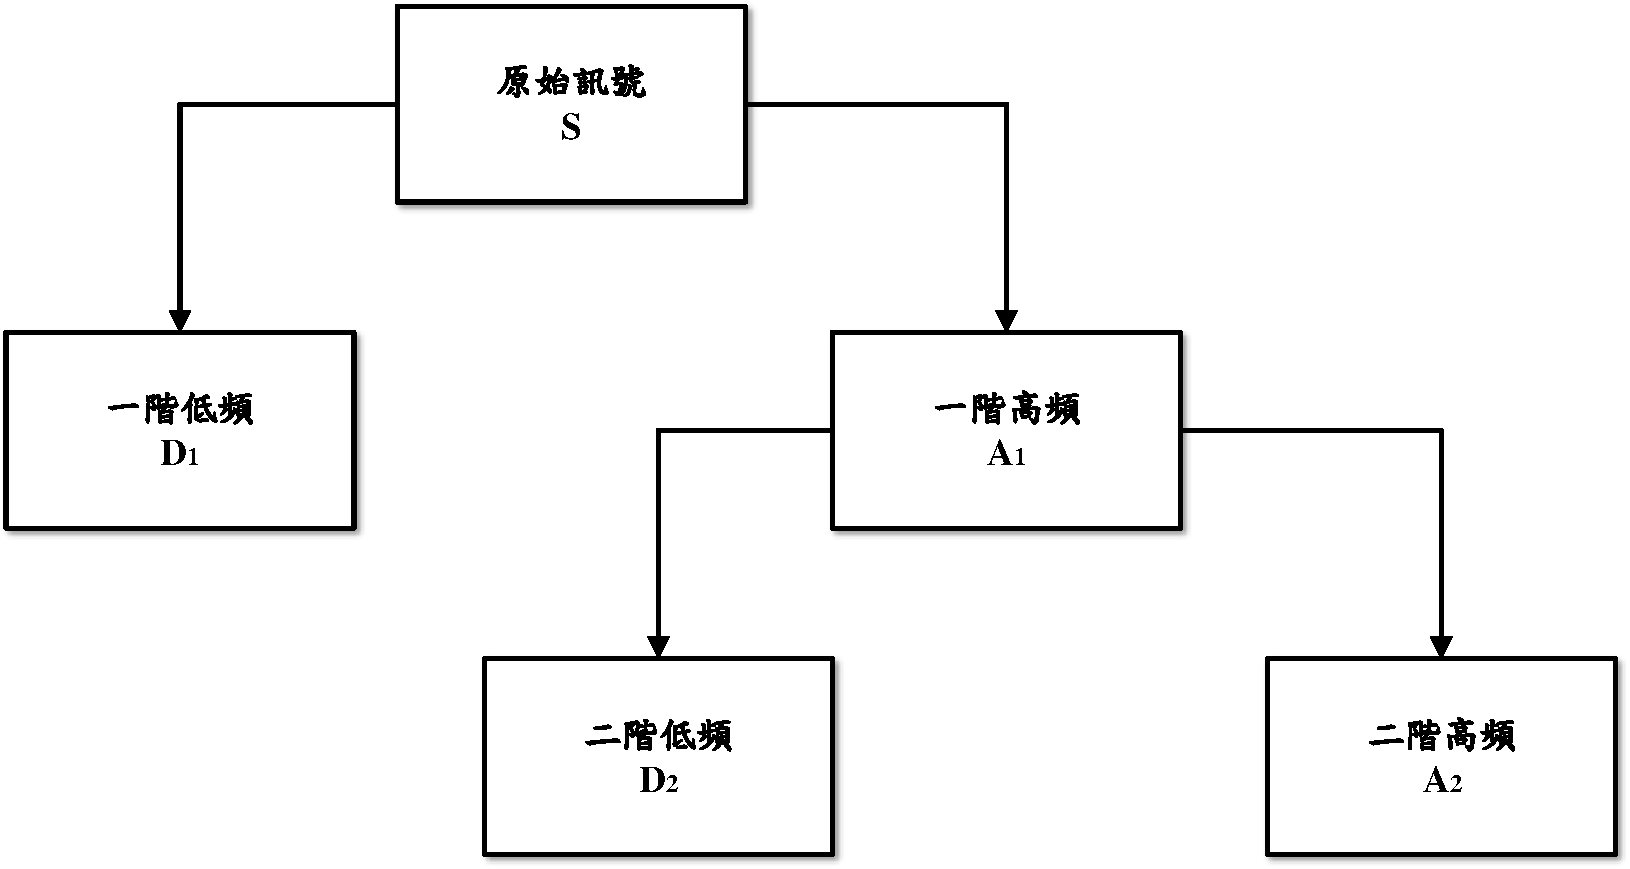
\includegraphics[width=0.9\textwidth]{Descrete Wavelet Transform}
  \caption{離散小波轉換階層架構}
  \label{figure: Descrete Wavelet Transform}
\end{figure}

\subsection{時間序列模型}

\subsubsection{時間序列預測(Time Series Prediction Model)}

將資料按照一定的時間間隔與發生順序紀錄而成的數列稱為時間序列(time series),時間序列預測透過序列本身所具有的時序性和自相關性,基於已知事件建構數學模型找出趨勢以確定未來事件 \cite{Wang2012}。一個基本的時間序列預測模型方程式 \eqref{equation: Time Series Prediction Model} 所示 \cite{box2015time}:

\begin{equation}\label{equation: Time Series Prediction Model}
  \hat{y} (t + T) = f\Big( y(t), y(t - T), \dots, y(t - mT) \Big)
\end{equation}

其中,$T$ 為取樣的時間間隔;$\hat{y}(t + T)$ 為預測值;$y(t)$、$y(t - T)$、$\dots$、$y(t - mT)$ 為當下的實際觀測值與過去時刻的實際觀測值;$m$ 值決定採用之前多少時刻的觀測值來進行預測。

方程式 \eqref{equation: Time Series Prediction Model} 表示:未來某一時刻的預測值僅依賴於前 $m$ 個時刻的歷史觀測值。

\subsubsection{平穩性與非平穩性(Stationary and Non-Stationary)}

時間序列通常存在非平穩性(nonstationarity)與時間波動(time-varying volatility)的特徵導致分析困難,若時間序列的統計特徵指標與時間無關,不會因為時間改變而變動,稱其具備平穩性或稱為恆定性。穩定性依據其形態分為強穩定性與弱穩定性,一般統計學中定義採用弱穩定性(weakly stationary):若時間序列 $\{ Y_t \}$ 滿足方程式 \eqref{equation: Stationary Condition},則稱時間序列 $\{ Y_t \}$ 是平穩的。

\begin{subequations}\label{equation: Stationary Condition}
  \begin{alignat}{2}
    E(Y_t) = E(Y_{t - s}) = \mu                                                  \qquad & \text{, } \forall~t, s \in \mathbb{N} \\
    E(Y_t - \mu)(Y_t - \mu) = E(Y_{t-s} - \mu)(Y_{t-s} - \mu) = \sigma_{y}^{2}   \qquad & \text{, } \forall~t, s \in \mathbb{N} \\
    E(Y_t - \mu)(Y_{t-s} - \mu) = E(Y_{t-j} - \mu)(Y_{t-j-s} - \mu) = \gamma_{s} \qquad & \text{, } \forall~t, s, j \in \mathbb{N}
  \end{alignat}
\end{subequations}

方程式 \eqref{equation: Stationary Condition} 表示平穩時間序列的期望值 $\mu$、變異數 $\sigma_{y}^{2}$ 和自相關係數 $\gamma_r$ 均為常數,不因時間的變動而改變。

\subsubsection{模型分類}

一般將時間序列根據其是否滿足平穩性條件分為平穩性時間序列(Stationary Time Series)與非平穩時間序列(Non-stationary Time Series),並依此決定採用的時間序列預測模型。平穩性時間序列多採用自迴歸模型(AR)、移動平均模型(MA)或自迴歸移動平均模型(ARMA);而非平穩時間序列需要透過差分運算使時間序列滿足平穩性,採用差分移動自迴歸模型(ARIMA)。

\paragraph{自迴歸模型(Autoregressive Model, AR Model)} 

使用時間序列自身作為迴歸變數,依賴於本身延遲的的滯後項和當前時間的干擾項對未來數值進行預測,其模型如方程式 \eqref{equation: AR Model} 所示,適用於平穩性時間序列。

\begin{equation}\label{equation: AR Model}
  \begin{split}
    \hat{y}_{t} & = c + \sum_{i = 1}^{p} \phi_{i} y_{t-i} + \epsilon_{t} \\
                & = c + \phi_{1} y_{t-1} + \phi_{2} y_{t-2} + \cdots + \phi_{p} y_{t-p} + \epsilon_{t}
  \end{split}
\end{equation}

其中,$c$ 為常數項;$\phi_i~(i = 1, 2, \ldots, p)$ 為自相關係數;$y_{t - i}~(i = 1, 2, \ldots, p)$ 為時間序列中過去時刻的觀測值;$\epsilon_t$ 為當前時間的干擾項,代表無法由過去時刻資料所解釋的雜訊或白噪聲;$p$ 為模型的自迴歸階數。一個 $p$ 階的自迴歸模型記為 $\text{AR} (p)$。

\paragraph{移動平均模型(Moving-Average Model, MA Model)}

主要依賴於過去與當前時間的干擾項,對不同時期的雜訊或噪聲給予不同的權重來進行線性組合,其模型如方程式 \eqref{equation: AR Model} 所示,適用於平穩性時間序列。

\begin{equation}\label{equation: MA Model}
  \begin{split}
    \hat{y}_{t} & = c + \sum_{j = 1}^{q} \theta_{j} \epsilon_{t-j} + \epsilon_{t} \\
                & = c + \theta_{1} \epsilon_{t-1} + \theta_{2} \epsilon_{t-2} + \cdots + \theta_{q} \epsilon_{t-q} + \epsilon_{t}
  \end{split}
\end{equation}

其中,$\mu$ 為時間序列的平均值;$\theta_{j}~(j = 1, 2, \ldots, q)$ 為移動平均係數;$\epsilon_{t - j}~(j = 1, 2, \ldots, q)$ 和 $\epsilon_t$ 分別為時間序列中過去時刻與當前時間的干擾項,代表雜訊或白噪聲;$q$ 為模型的滑動平均階數。一個 $q$ 階的移動平均模型記為 $\text{MA} (q)$。

\paragraph{自迴歸移動平均模型(Autoregressive Moving-Average Model, ARMA Model)}

採用了自迴歸模型與移動平均模型作為基礎,可以視為是兩個模型的線性組合,其模型如方程式 \eqref{equation: ARMA Model} 所示,適用於平穩性時間序列。

\begin{equation}\label{equation: ARMA Model}
  \hat{y}_{t} = \mu + \sum_{i = 1}^{p} \phi_{i} y_{t-i} + \sum_{j = 1}^{q} \theta_{j} \epsilon_{t-j} + \epsilon_{t}
\end{equation}

其中,分別引入了方程式 \eqref{equation: AR Model} 和 \eqref{equation: MA Model} 所表示自迴歸模型與移動平均模型。一個包含了 $p$ 階自迴歸項和 $q$ 階的移動平均項的自迴歸移動平均模型記為 $\text{ARMA} (p, q)$。

\paragraph{整合自迴歸移動平均模型(Autoregressive Integrated Moving-Average Model, ARIMA Model)}

將非平穩時間序列透過方程式 \eqref{equation: First Order Difference Series} 的差分處理,使其具備平穩性之後再建立自迴歸移動平均模型,其模型如方程式 \eqref{equation: ARIMA Model} 所示,適用於非平穩性時間序列。

\begin{equation}\label{equation: First Order Difference Series}
  {y}_{t}^{(d)} = y_{t}^{(d-1)} - y_{t-1}^{(d-1)}
\end{equation}

\begin{equation}\label{equation: ARIMA Model}
  \hat{y}_{t}^{(d)} = c + \sum_{i = 1}^{p} \phi_{i} {y}_{t-i}^{(d)} + \sum_{j = 1}^{q} \theta_{j} \epsilon_{t-j} + \epsilon_{t}
\end{equation}

其中,分別引入了方程式 \eqref{equation: AR Model} 和 \eqref{equation: MA Model} 所表示自迴歸模型與移動平均模型,並使用差分處理後的時間序列進行預測;$d$ 表示整合階數。一個經 $d$ 次差分後方使具備平穩性,包含了 $p$ 階自迴歸項和 $q$ 階的移動平均項的整合自迴歸移動平均模型記為 $\text{ARIMA} (p, d, q)$。

\subsubsection{平穩性檢驗(Stationary Testing)}

實務上在檢驗時間序列的平穩性時,會使用圖形檢驗法或單根檢驗法。圖形檢驗法透過觀察時間序列的走勢圖來判斷是否存在趨勢性與週期性,根據觀察者不同而有主觀性差異;單根檢驗法透過比較時間序列特徵根與單位圓位置關係判斷平穩性,實證分析中常用的單根檢定方法有:Dickey-Fuller 檢定(DF 檢定)、Augmented Dickey-Fuller 檢定(ADF 檢定)、Phillips-Perron 檢定(PP 檢定)、Kwiatkowski, Phillips, Schmidt \& Shin 檢定(KPSS 檢定)、Elliott-Rothenberg-Stock Point-Optimal 檢定(ERS Point-Optimal 檢定)和 Ng-Perron 檢定(NP 檢定)…等,以下針對本研究中所使用的 ADF 檢定與 KPSS 檢定進行說明。

\paragraph{Augmented Dickey-Fuller 檢定(ADF 檢定)} 

延伸自 DF 檢定,修正了一般 DF 檢定只能用於檢驗一階時間序列相關穩定性的設定,因此可以用於檢測存在高階時間序列相關的穩定性。根據常數項或時間趨勢的有無,分為以下三種型態:

\begin{enumerate}
  \item \textbf{無常數項以及時間趨勢}
    \begin{equation}
      \hat{y}_{t} = \beta y_{t - 1} + \sum_{j = 1}^{p - 1} \zeta_{j} \Delta y_{t - j} + \epsilon_{t} \quad \text{, } \epsilon_{t} \sim \mathcal{WN}(0, \sigma^2)
    \end{equation}
  \item \textbf{含常數項但無時間趨勢}
    \begin{equation}
      \hat{y}_{t} = \mu + \beta y_{t - 1} \sum_{j = 1}^{p - 1} \zeta_{j} \Delta y_{t - j} + \epsilon_{t} \quad \text{, } \epsilon_{t} \sim WN(0, \sigma^2)
    \end{equation}
  \item \textbf{含常數項以及時間趨勢}
    \begin{equation}
      \hat{y}_{t} = \mu + \alpha t + \beta y_{t - 1} + \sum_{j = 1}^{p - 1} \zeta_{j} \Delta y_{t - j} + \epsilon_{t} \quad \text{, } \epsilon_{t} \sim WN(0, \sigma^2)
    \end{equation}
\end{enumerate}

對於上述三個迴歸模型,其假設檢定為虛無假設 $H_0$:$\beta = 1$,對立假設 $H_1: \beta < 1$,若取 $y_{t-1}$ 項 OLS 估計法下的 $t$ 檢驗值作為 ADF 統計量值,如果 ADF 統計量小於臨界值,則說明其足夠小可以拒絕虛無假設,表示時間序列具備平穩性。

\paragraph{Kwiatkowski, Phillips, Schmidt \& Shin 檢定(KPSS 檢定)} 

有別於其他單根檢定法將虛無假設設為序列具有單根而傾向接受單根,改以變數滿足平穩作為其虛無假設,通常用來確認其他單根檢定法的檢定結果。假設迴歸模型如方程式 \eqref{equation: KPSS Regression} 所示:

\begin{equation}\label{equation: KPSS Regression}
  \hat{y}_{t} = \zeta t + u_{t}  + \epsilon_{t}
\end{equation}

其中 $\zeta_t$ 為一定向趨勢;$u_{t}$ 為一隨機漫步,即 $u_{t} = u_{t-1} + u_{t}$ 且 $u_t$ 為滿足獨立有共同分佈(independent and identically distributed) $i.i.d. (0, \sigma_{u}^{2})$ 的隨機變數;$\epsilon_{t}$ 為一定態白噪音。假設檢定為虛無假設 $H_0$:$\sigma_{u}^{2} = 0$,對立假設 $H_1: \sigma_{u}^{2} > 1$,在此虛無假設為真的前提下可以推導出方程式 \eqref{equation: KPSS LM} 所示的 KPSS 檢定統計式。

\begin{equation}\label{equation: KPSS LM}
  LM = \frac{\sum_{t = 1}^{T} S_{t}^{2}}{\hat{\sigma}_{\epsilon}^{2}}
\end{equation}

其中 $S_t$ 為殘差的累計總合;$\hat{\sigma}_{\epsilon}^{2}$ 為長期殘差變異數的估計值,在 KPSS 檢定中採用 Bartlett windows 準則來構建加權函數 $w(s, l) = 1 - s/(l + 1)$。KPSS 檢定法推導出上述檢定統計量的漸進分配並模擬出臨界值表,此檢定為右尾檢定,若檢定落於臨界值外則拒絕虛無假設,表示時間序列不具備平穩性,需進行差分處理。

\subsubsection{模型識別(Model Identification)}

前述介紹的時間序列預測模型,最終皆能夠以整合自迴歸移動平均模型表示為 $\text{ARIMA}(p, d, q)$ 的形式,表 \ref{table: Special Case of ARIMA(p, q, r)} 為整合自迴歸移動平均模型在選用特定階數時的特例與退化後的結果。

\begin{table}[htp]
  \centering
  \caption[整合自迴歸移動平均模型的特例]{整合自迴歸移動平均模型的特例}
  \begin{tabular*}{\textwidth}{cl}
    \toprule
    \textbf{模型}           & \textbf{說明}                     \\
    \midrule
    $\text{ARIMA}(0, 0, 0)$ & 白噪聲(white noise)             \\
    $\text{ARIMA}(0, 1, 0)$ & 隨機漫步模型(random walk)       \\
    $\text{ARIMA}(p, 0, 0)$ & 自迴歸模型(AR Model)            \\
    $\text{ARIMA}(0, 0, q)$ & 移動平均模型(MA Model)          \\
    $\text{ARIMA}(p, 0, q)$ & 自迴歸移動平均模型(ARMA Model)  \\
    \bottomrule
  \end{tabular*}
  \label{table: Special Case of ARIMA(p, q, r)}
\end{table}

所謂的模型識別(model identification)即是指決定整合自迴歸移動平均模型 $\text{ARIMA}(p, d, q)$ 中階數的過程,此一階段將採用 Box-Jenkins 方法,透過自相關函數(Autocorrelation Function, ACF)與偏相關函數(Partial Autocorrelation Function, PACF)及其對應的相關圖形進行判斷。

\paragraph{自相關函數(Autocorrelation Function, ACF)} 

反映了同一時間序列在不同時刻取值的相關程度,定義為第 $k$ 個時間差的自協方差函數與標準差的商值,如方程式 \eqref{equation: Autocorrelation Function} 所示。

\begin{equation}\label{equation: Autocorrelation Function}
  \rho_{k} = \frac{\mathrm{Cov}(y_t, y_{t + k})}{\sqrt{\mathrm{Var}(y_{t})\mathrm{Var}(y_{t+k})}} = \frac{\gamma_{k}}{\sigma_{y}^{2}}
\end{equation}

對於 $\text{AR}(p)$ 模型而言,其自相關函數會隨著階數 $p$ 的增加而逐步衰減但不為零,呈現拖尾(tail off)的性質;而對於 $\text{MA}(q)$ 模型而言,其自相關函數會在階數 $q$ 之後為零,呈現截尾(cut off)的性質。

\paragraph{偏相關函數(Partial Autocorrelation Function, PACF} 

定義為移除額外變數的影響後,時間序列 $\{ y_t \}$ 與滯後 $k$ 階時間序列 $\{ y_{t-k} \}$ 的線性相關程度,通常以 $\phi_{kk}$ 來表示時間序列的偏相關函數,定義如方程式 \eqref{equation: Partial Autocorrelation Function} 所示。

\begin{equation}\label{equation: Partial Autocorrelation Function}
  \phi_{kk} = \frac{\mathrm{Cov}(y_t, y_{t-k} | y_{t-1}, y_{t-2}, \cdots, y_{t-k+1})}{\sigma_{y_{t} | y_{t-1}, y_{t-2}, \cdots, y_{t-k+1}} \sigma_{y_{t-k} | y_{t-1}, y_{t-2}, \cdots, y_{t-k+1}}}
\end{equation}

對於 $\text{AR}(p)$ 模型而言,其偏相關函數會會在階數 $q$ 之後為零,呈現截尾(cut off)的性質;而對於 $\text{MA}(q)$ 模型而言,其偏相關函數會隨著階數 $p$ 的增加而逐步衰減但不為零,呈現拖尾(tail off)的性質。

由於平穩時間序列的自相關函數與偏相關函數分別具有不同特徵,在進行模型識別的過程中通常觀察其自相關函數圖形與偏相關函數圖形的特徵,比如是否截尾以及在何處截尾來決定模型的類型與具體階數,表 \ref{table: Characteristic of ACF and PACF} 整合自迴歸移動平均模型的 ACF 與 PACF 圖形判斷準則。

\begin{table}[htp]
  \centering
  \caption[自相關函數與偏相關函數之特徵]{自相關函數與偏相關函數之特徵}
  \begin{tabular*}{\textwidth}{cll}
    \toprule
    \textbf{模型} & \textbf{自相關函數(ACF)} & \textbf{偏相關函數(PACF)} \\
    \midrule
    \text{AR} (p) & 指數衰減或振盪,具有拖尾性 & 在 $p$ 階截尾,自 $p$ 階後明顯消失 \\
    \text{MA} (q) & 在 $q$ 階截尾,自 $q$ 階後明顯消失 & 指數衰減或振盪,具有拖尾性 \\
    \text{ARMA} (p, q) & 指數衰減或振盪,具有拖尾性 & 指數衰減或振盪,具有拖尾性 \\
    \bottomrule
  \end{tabular*}
  \label{table: Characteristic of ACF and PACF}
\end{table}

透過 ACF 與 PCAF 圖形特徵進行初步階數選定之後,需要從眾多可選的模型中選出最適模型,此時需要使用方程式 \eqref{equation: AIC and BIC} 所示的 AIC(Akaike's Information Criterion)及 BIC(Bayesian Information Criterion)作為評價模型優劣的指標。

\begin{equation}\label{equation: AIC and BIC}
  \begin{split}
    \text{AIC} & = -2 \ln{L} + 2k       \\
    \text{BIC} & = -2 \ln{L} + k \ln{n}
  \end{split}
\end{equation}

其中,$L$ 為模型似然函數(Likelihood Function),表示模型擬合指標;$k$ 為滯後期數總和,作為自由度懲罰項避免模型發生過度擬合的情況。

\subsection{支持向量迴歸}

支持向量機(Support Vector Machine, SVM)是機器學習領域中的監督式學習方法,根據統計學習理論中的結構風險最小化原則提出,目前被廣泛應用於統計學上的分類(classification)與迴歸分析(regression analysis)中。

\subsubsection{支持向量機(Support Vector Machine, SVM)}

給定一組數據 $\{ (\boldsymbol{x}_1, y_1), (\boldsymbol{x}_2, y_2), \ldots, (\boldsymbol{x}_{m}, y_m) \}$,其中 $\boldsymbol{x}_{i} \in \mathbb{R}^d, y_i \in \{-1, 1\}$,空間中可以找到一劃分超平面 $\boldsymbol{w}^{\top} \boldsymbol{x}_i + b = 0$ 將其分開。對於 $\mathbb{R}^d$ 空間中某點 $\boldsymbol{p} \in \mathbb{R}^d$ 到劃分超平面 $\boldsymbol{w}^{\top} \boldsymbol{x}_i + b = 0$ 的距離可以表示為方程式 \eqref{equation: Distance Between Plane and Point} 所示。

\begin{equation}\label{equation: Distance Between Plane and Point}
  d = \frac{1}{\norm{\boldsymbol{w}}} \abs{\boldsymbol{w}^{\top} \boldsymbol{p} + b}
\end{equation}

為求解上述的線性分類問題,支持向量機定義間隔(margin)為距離劃分超平面最近樣本點到劃分超平面距離的兩倍,如方程式 \eqref{equation: SVM Margin} 所示,用以表示劃分超平面到不同標記之最近樣本點的距離總和。

\begin{equation}\label{equation: SVM Margin}
  \gamma \coloneqq 2 \min_{i} \frac{1}{\norm{\boldsymbol{w}}} \abs{\boldsymbol{w}^{\top} \boldsymbol{x}_i + b}
\end{equation}

經過簡化後,原有線性二分問題可以轉為限制條件為線性方程式的最佳化模型,如方程式 \eqref{equation: Support Vector Model} 所示。

\begin{equation}\label{equation: Support Vector Model}
  \begin{aligned}
    \max_{\boldsymbol{w}, b} \qquad & \frac{1}{2} \boldsymbol{w}^{\top}\boldsymbol{w} \\
    \text{s.t.}              \qquad & y_i (\boldsymbol{w}^{\top} + b) \geq 1,\quad i = 1, 2, \ldots, m
  \end{aligned}
\end{equation}

圖 \ref{figure: Support Vector Machine} 為二維平面上一個最優分類線的示意圖,其中藍色與褐色的點表示兩類樣本中的樣本點,直線 $L_1$ 與 $L_2$ 則分別代表兩類樣本中平行於分類線並與其距離最小的直線,兩者間距 $d_{12}$ 可以表示為方程式 \eqref{equation: Distance between Two Line},此間隔必須滿足 $2 / \norm{w}$,亦即保證分類間隔最大與使得 $\frac{1}{2} \norm{w}^2$ 最小具有相同的意義;在高維空間中的分類線將變為一個分類面。

\begin{equation}\label{equation: Distance between Two Line}
  d_{12} = \min_{x_i, y_j = 1} \frac{\abs{w\cdot x_i + b}}{\norm{w}} + \min_{x_i, y_j = -1} \frac{\abs{w\cdot x_j + b}}{\norm{w}}
\end{equation}

\begin{figure}[htbp]
  \centering
  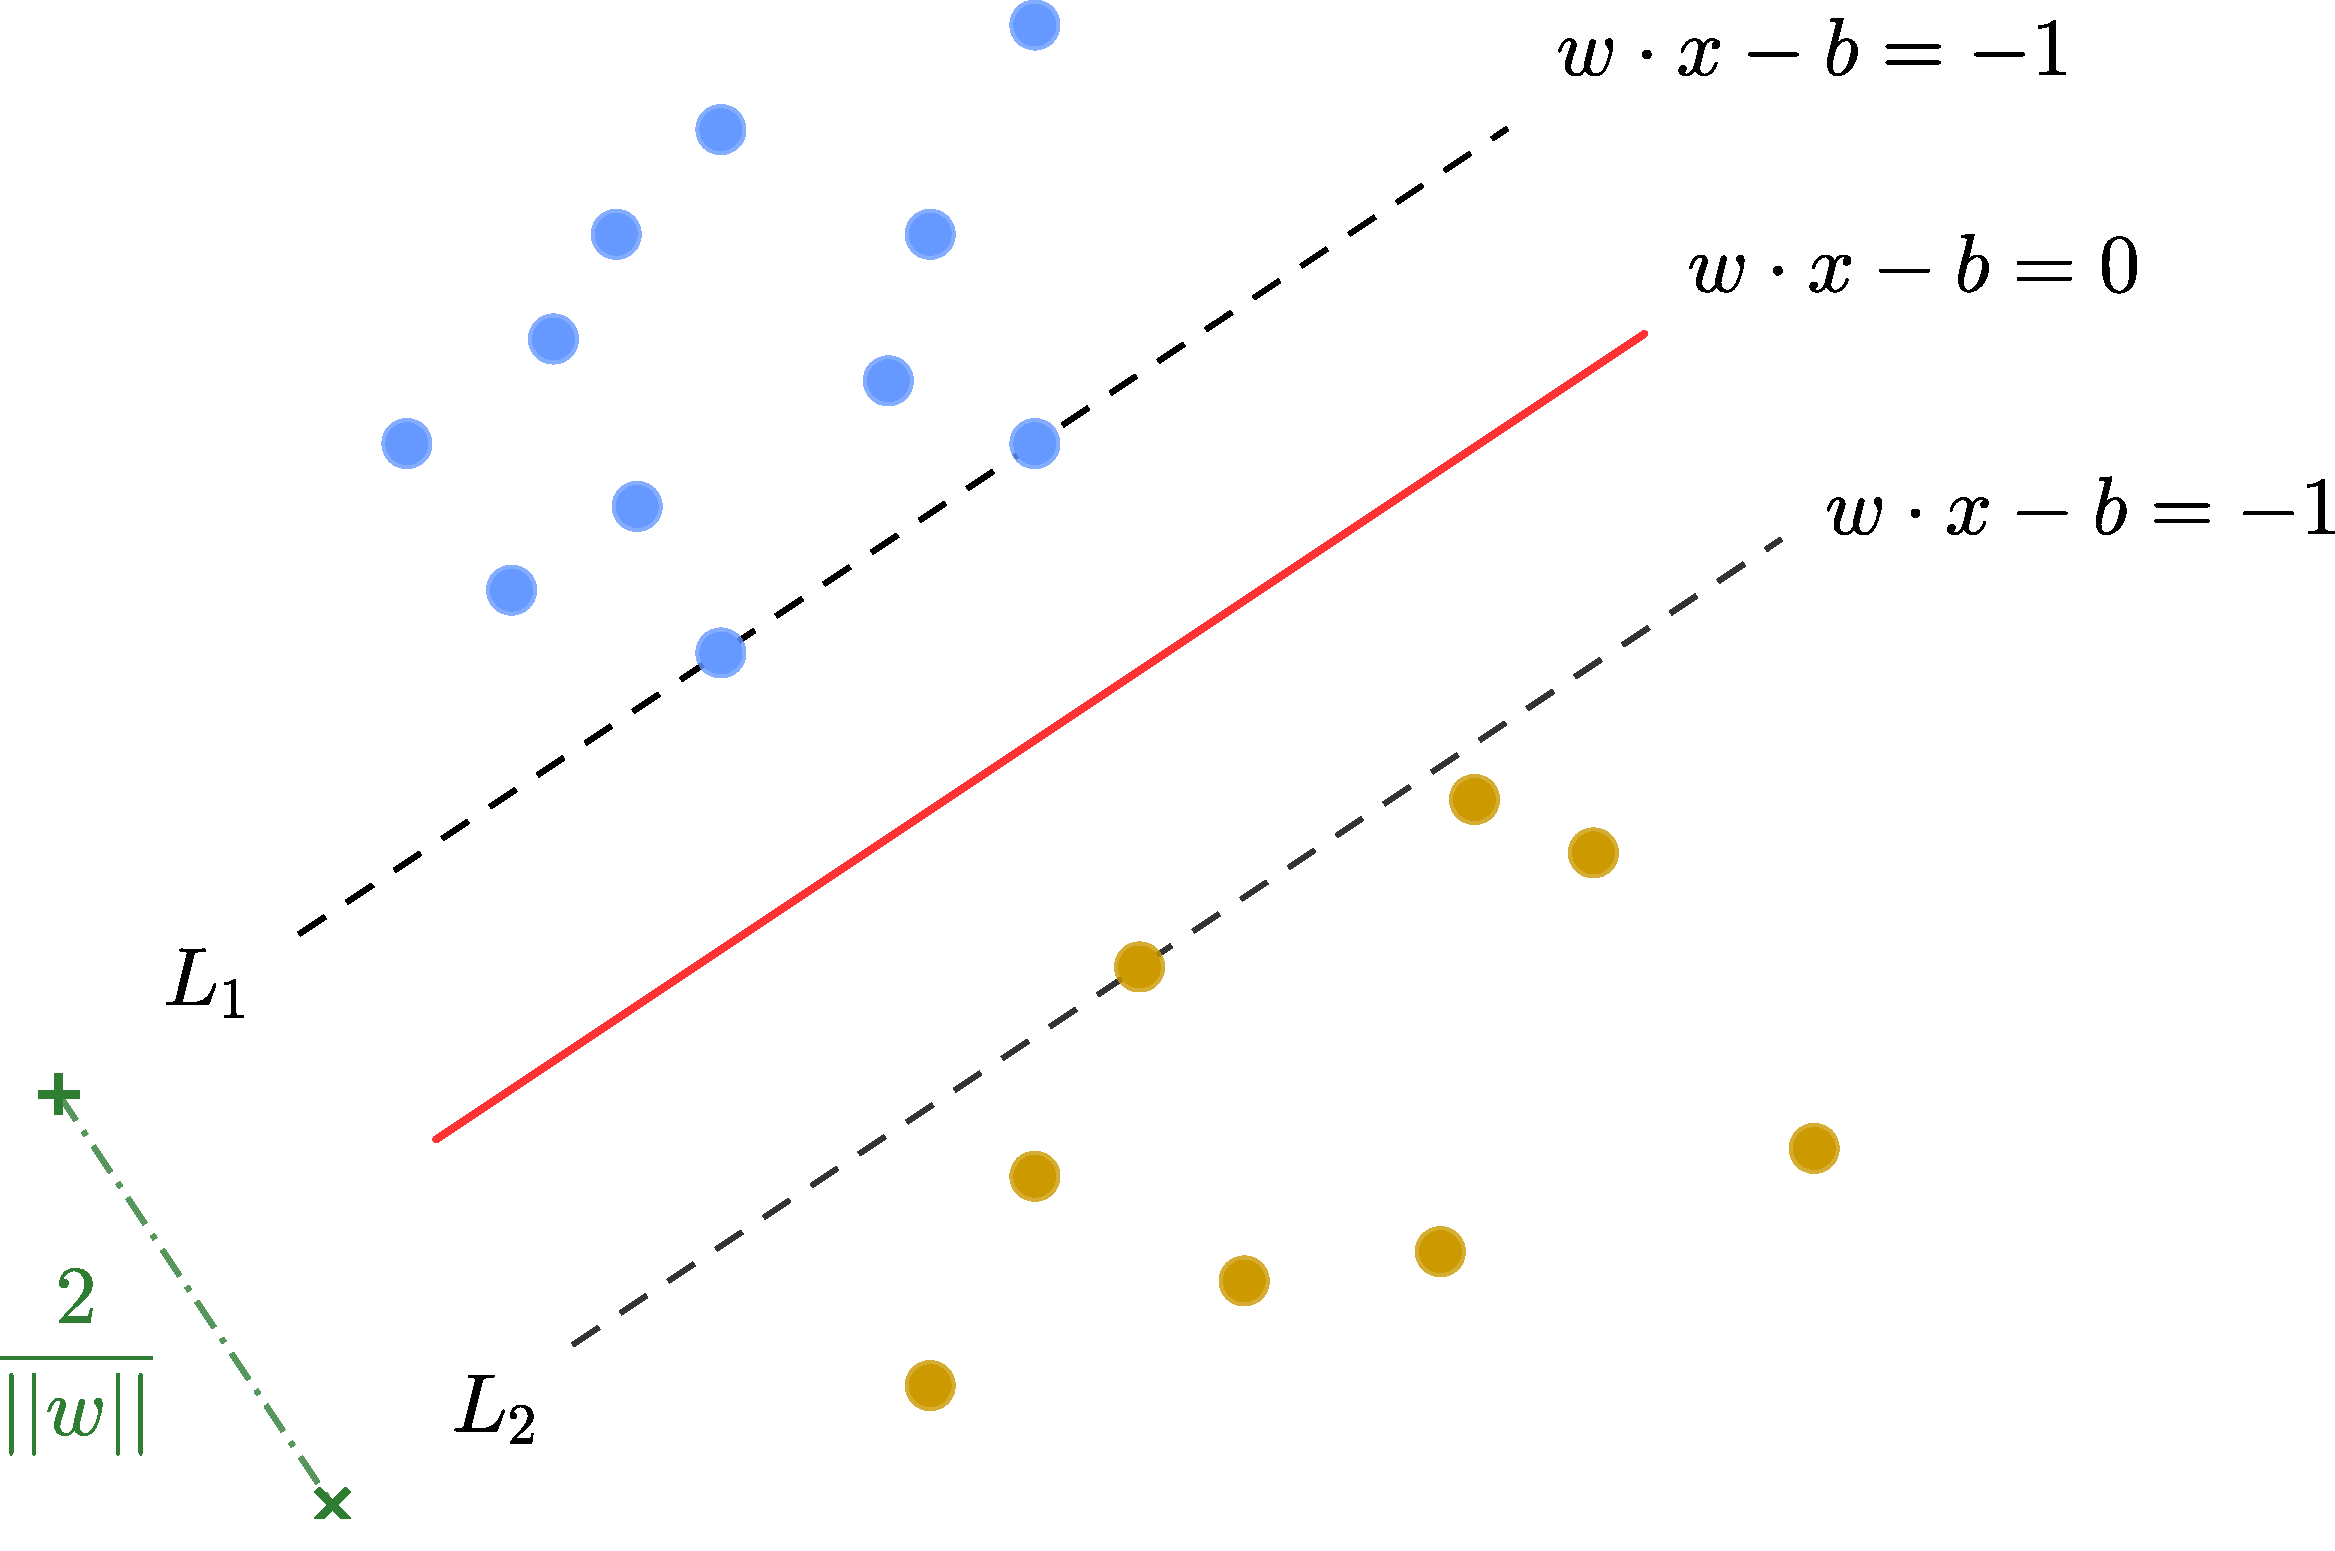
\includegraphics[width=0.8\textwidth]{Support Vector Machine}
  \caption[二維平面上最優分類線]{二維平面上最優分類線}
  \label{figure: Support Vector Machine}
\end{figure}

對於帶有限制條件的最佳化問題,通常會構造其拉格朗日函數(Lagrange Function)進行求解,而引入拉格朗日函數後的規劃問題在極值處必須滿足庫恩塔克條件(Karush-Kuhn-Tucker Conditions, KKT Conditions);除此之外,由於線性支持向量機滿足 Slater 條件,其對偶問題將等價於原問題。因此一個線性支持向量機的對偶形式即找到一組合適的 $\boldsymbol{\alpha}$ 滿足方程式 \eqref{equation: Dual SVM Problem} 所示的最佳化問題。

\begin{equation}\label{equation: Dual SVM Problem}
  \begin{aligned}
    \min_{\boldsymbol{\alpha}} \qquad & \frac{1}{2} \sum_{i = 1}^{m} \sum_{j = 1}^{m} \alpha_i \alpha_j y_i y_j \boldsymbol{x}_i^{\top} \boldsymbol{x}_j - \sum_{i = 1}^{m} \alpha_{i} \\
    \text{s.t.}                \qquad & \sum_{i = 1}^{m} \alpha_{i} y_{i} = 0 \\
                               \qquad & \alpha_{i} \geq 0 ,\quad i = 1, 2, \ldots, m
  \end{aligned}
\end{equation}

此時若依據庫恩塔克條件(Karush-Kuhn-Tucker Conditions, KKT Conditions)進行求解,所得到的最優分類函數便如方程式 \eqref{equation: SVM Function} 所示。

\begin{equation}\label{equation: SVM Function}
  h(\boldsymbol{x}) = \text{sgn} \left( \sum_{i \in SV}^{m} \alpha_{i}y_{i} \boldsymbol{x}_{i}^{\top} \boldsymbol{x}_{i} + b \right)
\end{equation}

定義支持向量(Support Vector)為對偶變數 $\alpha_{i} \geq 0$ 所對應的樣本,上式中的 $SV$ 即代表所有支持向量所組成的集合。

\subsubsection{核函數(Kernal Functions)}

在實際狀況中存在許多非線性可分的問題,因此不存在一個劃分超平面來將屬於不同標記的訓練樣本點進行分開,在支持向量機中透過核技巧(Kernal Trick)將特徵空間 $\mathbb{R}^{d}$ 中非線性可分的樣本點映射至特徵空間 $\mathbb{R}^{\hat{d}}$ 中線性可分的樣本點,藉此來處理樣本非線性可分的狀況 \cite{boser1992training}。將樣本點進行適當地映射之後,支持向量機的基本型和對偶型將分別轉變為方程式 \eqref{equation: Non-Linear SVM Problem} 和方程式 \eqref{equation: Non-Linear Dual SVM Problem} 所示的最佳化問題。

\begin{equation}\label{equation: Non-Linear SVM Problem}
  \begin{aligned}
    \min_{\boldsymbol{w}, b} \qquad & \frac{1}{2} \boldsymbol{w}^{\top} \boldsymbol{w} \\
    \text{s.t.}              \qquad & y_{i} (\boldsymbol{w}^{\top} \boldsymbol{\phi} (\boldsymbol{x}_{i}) + b ) \geq 1 ,\quad i = 1, 2, \ldots, m
  \end{aligned}
\end{equation}

\begin{equation}\label{equation: Non-Linear Dual SVM Problem}
  \begin{aligned}
    \min_{\boldsymbol{\alpha}} \qquad & \frac{1}{2} \sum_{i = 1}^{m} \sum_{j = 1}^{m} \alpha_i \alpha_j y_i y_j \boldsymbol{\phi} (\boldsymbol{x}_{i})^{\top} \boldsymbol{\phi} (\boldsymbol{x}_{j}) - \sum_{i = 1}^{m} \alpha_{i} \\
    \text{s.t.}                \qquad & \sum_{i = 1}^{m} \alpha_{i} y_{i} = 0 \\
                               \qquad & \alpha_{i} \geq 0 ,\quad i = 1, 2, \ldots, m
  \end{aligned}
\end{equation}

其中,$\boldsymbol{\phi} (\boldsymbol{x}_{i})$ 表示將樣本 $\boldsymbol{x}$ 映射至特徵空間 $\mathbb{R}^{\hat{d}}$ 中的特徵向量。為使計算時的複雜度降低,核技巧透過塑造一個形如方程式 \eqref{equation: Kernal Function} 所示的核函數(Kernal Function),將特徵映射與內積運算壓縮為一個步驟。

\begin{equation}\label{equation: Kernal Function}
  \kappa (\boldsymbol{x}_{i}, \boldsymbol{x}_{j}) = \boldsymbol{\phi} (\boldsymbol{x}_{i})^{\top} \boldsymbol{\phi} (\boldsymbol{x}_{j})
\end{equation}

其中,核函數必須滿足 Mercer 條件(Mercer Condition),亦即對於任意核函數 $\kappa (\boldsymbol{x}_{i}, \boldsymbol{x}_{j})$ 所對應的矩陣 $\boldsymbol{K} \coloneqq [\kappa (\boldsymbol{x}_{i}, \boldsymbol{x}_{j})]_{m \times m} $ 必須為半正定的 \cite{cristianini2000introduction};除此之外,核函數也可以透過現有的核函數進行線性組合得到 \cite{lanckriet2004learning}。表 \ref{table: Kernal Functions} 為滿足 Mercer 條件的常見核函數。

\begin{table}[htp]
  \centering
  \caption[滿足 Mercer 條件的常見核函數]{滿足 Mercer 條件的常見核函數}
  \begin{tabular*}{\textwidth}{ccl}
    \toprule
    \textbf{名稱}   & \textbf{形式}            & \textbf{說明}          \\
    \midrule
    線性核函數      & $\boldsymbol{x}_{i}^{\top} \boldsymbol{x}_{j}$ & 容易實現並具高解釋性,但無法解決非線 \\
                    &   & 性可分問題            \\
    多項式核函數    & $\left( \beta \boldsymbol{x}_{i}^{\top} \boldsymbol{x}_{j} + \theta \right)^{n}$ & 使用維度 $n$ 來描述被映射空間複雜度,但 \\
                    &   & 參數太多,當維度太大時計算較不穩定 \\
    指數徑向核函數  & $\exp \left(-\frac{\norm{\boldsymbol{x}_{i} - \boldsymbol{x}_{j}}}{2\sigma^2} \right)$ & 沒有計算不穩定的問題,但計算速度較慢 \\ 
                    &   & 且容易過度擬合 \\
    高斯徑向核函數  & $\exp \left(-\frac{\norm{\boldsymbol{x}_{i} - \boldsymbol{x}_{j}}^2}{2\sigma^2} \right)$ & 沒有計算不穩定的問題,但計算速度較慢 \\ 
                    &   & 且容易過度擬合 \\
    Sigmoid 核函數  & $\tanh{\left( \beta \boldsymbol{x}_{i}^{\top} \boldsymbol{x}_{j} + \theta \right)}$ & 透過支持向量機實現了神經網路,結果與 \\
                    &   & 徑向核函數相似,但在某些參數下無效 \\
    \bottomrule
  \end{tabular*}
  \label{table: Kernal Functions}
\end{table}

在實際的機器學習過程中,核函數的選擇決定了計算的性能表現、模型的合適狀況以及預測的準確程度。核函數的選取主要依靠領域背景知識進行判斷,或者是採取交叉驗證法根據不同分析情況採用不同的核函數,目前在大多數的情況下將優先採用對於任意樣本都有較好學習能力的高斯徑向核函數。

\subsubsection{支持向量迴歸(Support Vector Regression, SVR)}

在分類問題中,支持向量機尋找一個劃分超平面將樣本點一分為二;而在迴歸問題中,支持向量機尋找的則是能夠準確預測資料分佈的平面。

假設訓練資料表示為 $\{ (\boldsymbol{x}_1, y_1), (\boldsymbol{x}_2, y_2), \ldots, (\boldsymbol{x}_{m}, y_m) \}$,其中 $\boldsymbol{x}_i$ 和 $y_i$ 分別表示第 $i$ 組資料的特徵和對應的迴歸值,且 $(\boldsymbol{x}_{i}, y_i ) \in \mathbb{R}^d \times \mathbb{R}$。支持向量迴歸能夠容忍預測值 $h(\boldsymbol{x}_i)$ 與迴歸值 $y_i$ 之間小於 $\epsilon$ 的偏差,並可以表示為方程式 \eqref{equation: Support Vector Regression} 所示的最佳化問題 \cite{drucker1997support}。

\begin{equation}\label{equation: Support Vector Regression}
  \begin{aligned}
    \min_{\boldsymbol{\omega}, b}   \qquad & \frac{1}{2} \norm{\boldsymbol{\omega}}^2 \\
    \text{s.t.}                     \qquad & \abs{y_i - (\boldsymbol{\omega}^{\top} \boldsymbol{x_i} + b)} \leq \epsilon ,\quad i = 1, 2, \ldots, m
  \end{aligned}
\end{equation}

同樣地,在構造其拉格朗日函數並使用核函數將非線性可分的訓練資料進行映射後,支持向量迴歸可以形式化為方程式 \eqref{equation: Support Vector Regression Model} 所示的最佳化模型。

\begin{equation}\label{equation: Support Vector Regression Model}
  \begin{aligned}
    \min_{\boldsymbol{\omega}, b}   \qquad & \frac{1}{m} \sum_{i = 1}^{m} \max{\left(0, \abs{y_i - (\boldsymbol{\omega}^{\top} \boldsymbol{\phi}(\boldsymbol{x}_i) + b)} - \epsilon \right)} + \frac{\lambda}{2} \boldsymbol{\omega}^{\top}\boldsymbol{\omega}
  \end{aligned}
\end{equation}

\subsection{模型評價方法}

評價預測模型的好壞是計算預測結果與實際數據之間的誤差,常見的模型評價方法有以下幾種:

\begin{enumerate}
  \item \textbf{均方根誤差(Root Mean Squares Error, RMSE)}:
    \begin{equation} \label{equation: RMSE}
      E_{\text{RMSE}} = \sqrt{\frac{1}{n} \sum_{t = 1}^{n} (y_t - \hat{y}_t)^2}
    \end{equation}
  \item \textbf{平均絕對百分比誤差}:
    \begin{equation} \label{equation: MAPE}
      E_{\text{MAPE}} = \frac{1}{n} \sum_{t = 1}^{n} \frac{\abs{y_t - \hat{y}_t}}{\abs{y_t}}
    \end{equation}
  \item \textbf{平均絕對誤差(Mean Absolute Error, MAE)}:
    \begin{equation} \label{equation: MAE}
      E_{\text{MAE}} = \frac{1}{n} \sum_{t = 1}^{n} \abs{y_t - \hat{y}_t}
    \end{equation}
  \item \textbf{誤差平均值}:
    \begin{equation} \label{equation: ME}
      E_{\text{ME}} = \frac{1}{n} \sum_{t = 1}^{n} (y_t - \hat{y}_t)
    \end{equation}
\end{enumerate}

\section{收益模型分析}

\subsection{自由電力市場}

早期世界各國的電力供應具有壟斷特性,直至二十世紀末歐美各國才紛紛重新組織電力產業,打破垂直整合的獨佔電力市場。自由電力市場會使得電力價格由市場機制決定,迫使電價下跌並推動電力設備升級,使用者也因此能受到更加專業與透明的電力服務。

\subsubsection{電力市場架構}

\begin{figure}
  \centering
  \begin{subfigure}[b]{0.475\textwidth}
    \centering
    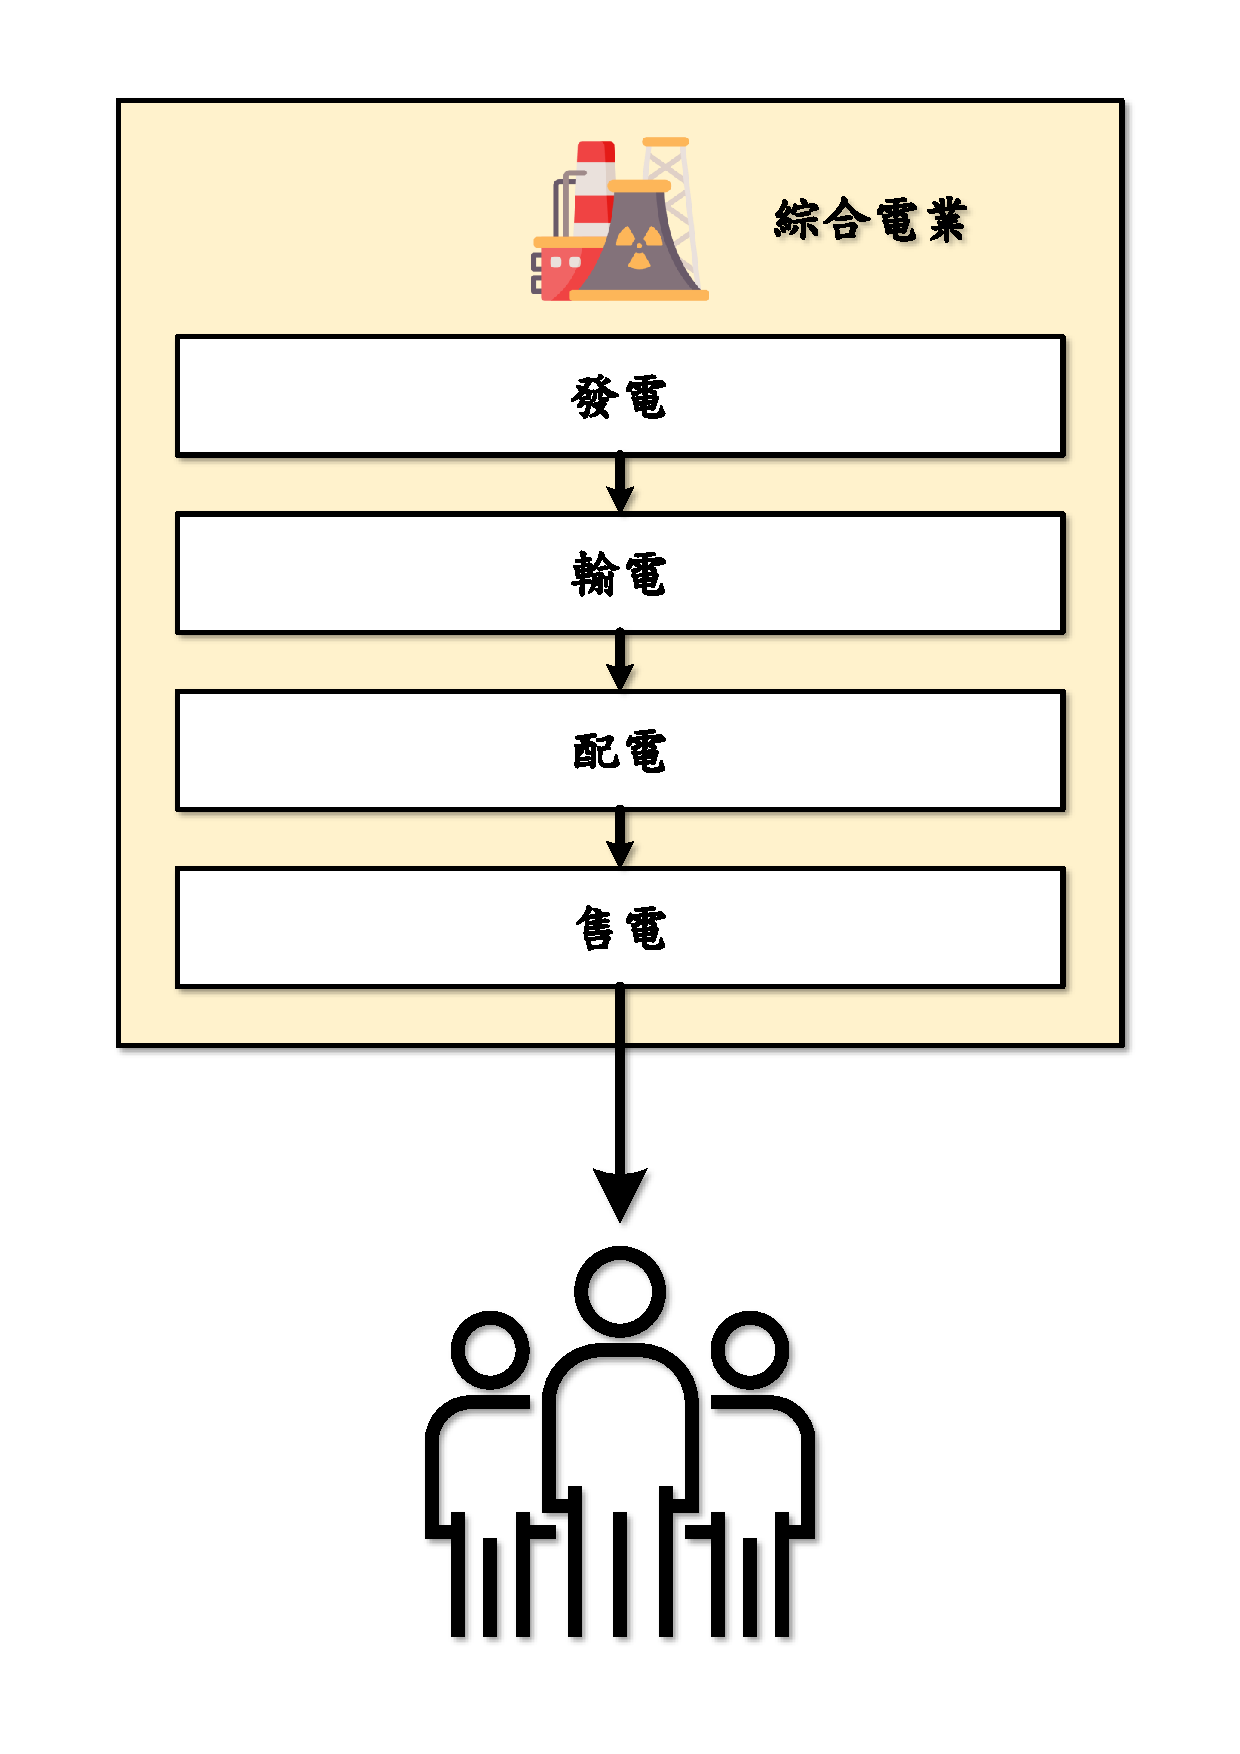
\includegraphics[width=\textwidth]{Power Monopoly Market}
    \caption[垂直壟斷]{垂直壟斷}
  \end{subfigure}
  \hfill
  \begin{subfigure}[b]{0.475\textwidth}
    \centering
    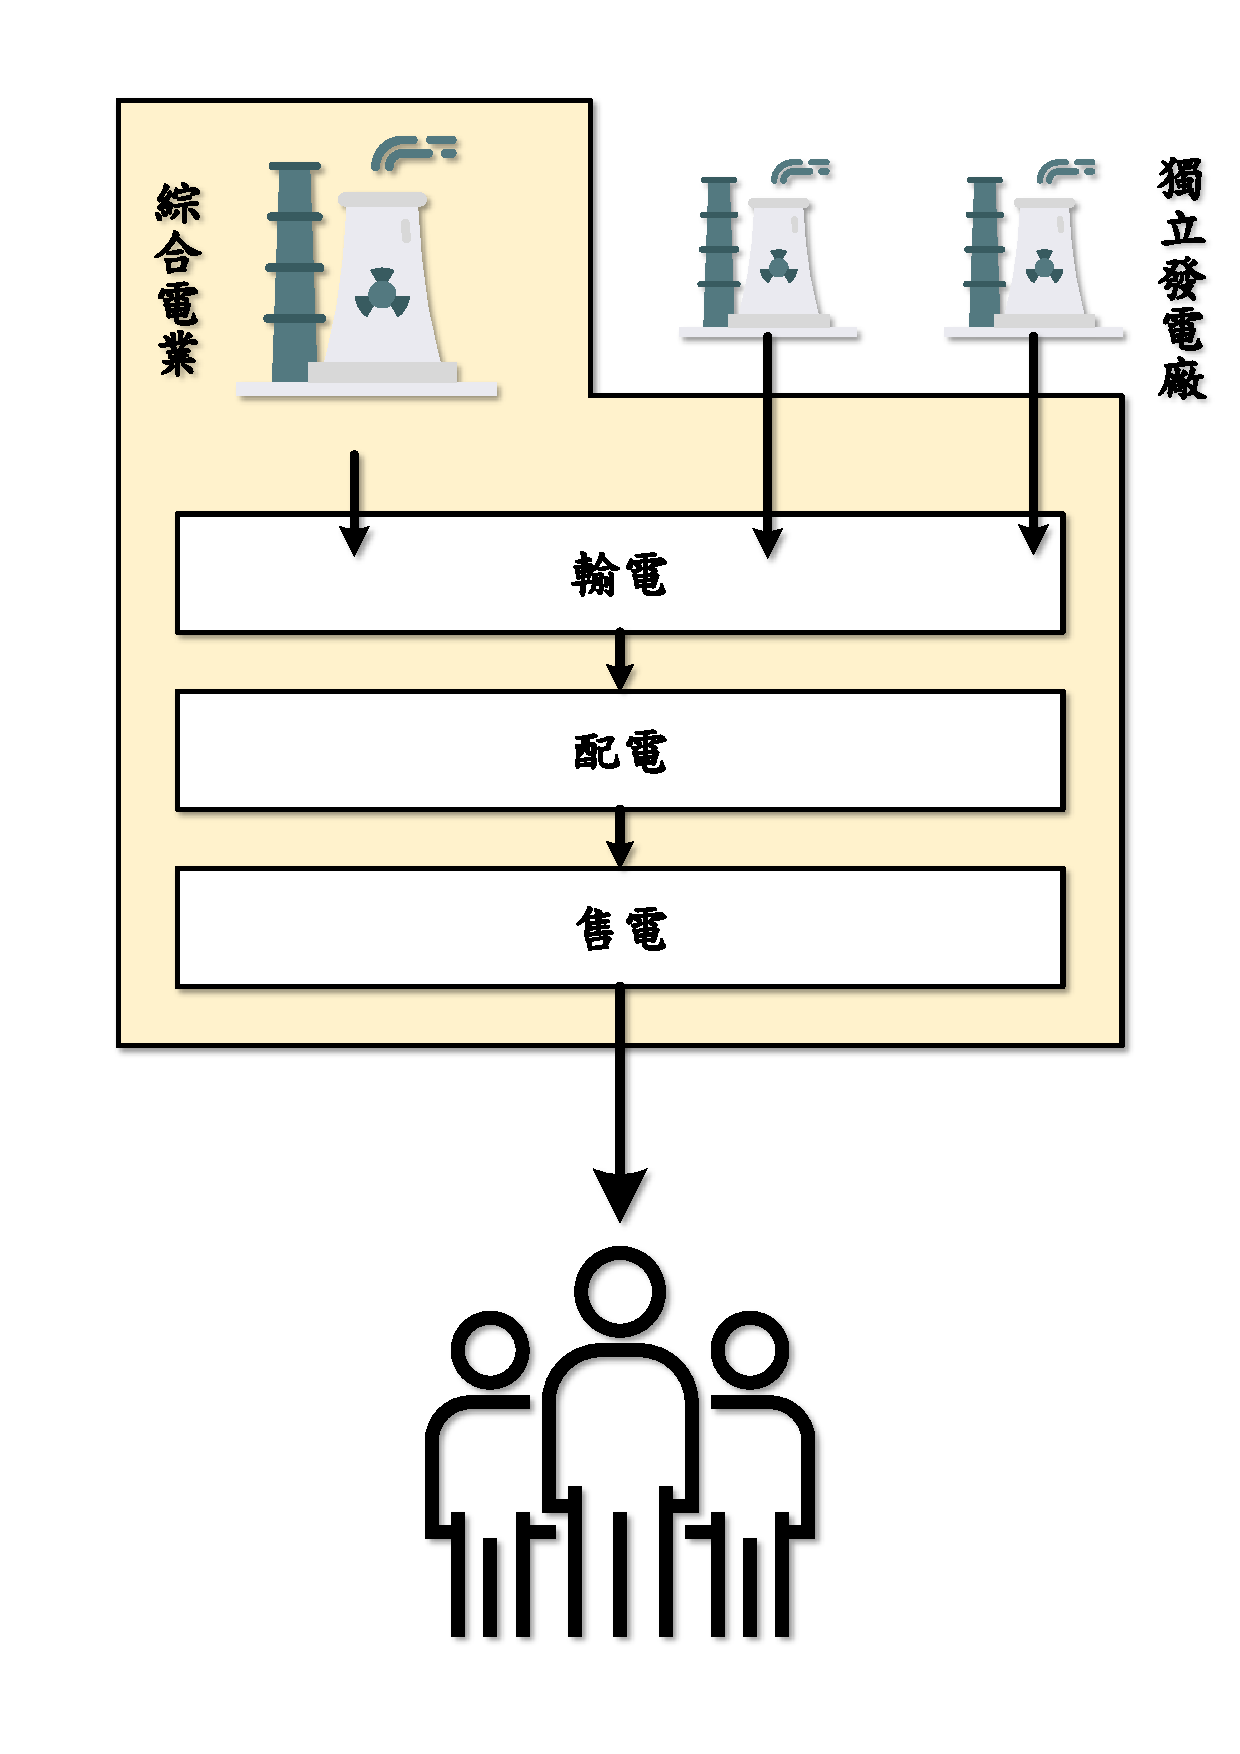
\includegraphics[width=\textwidth]{Power One-Buy Market}
    \caption[單一買方]{單一買方}
  \end{subfigure}
  \hfill
  \begin{subfigure}[c]{0.475\textwidth}
    \centering
    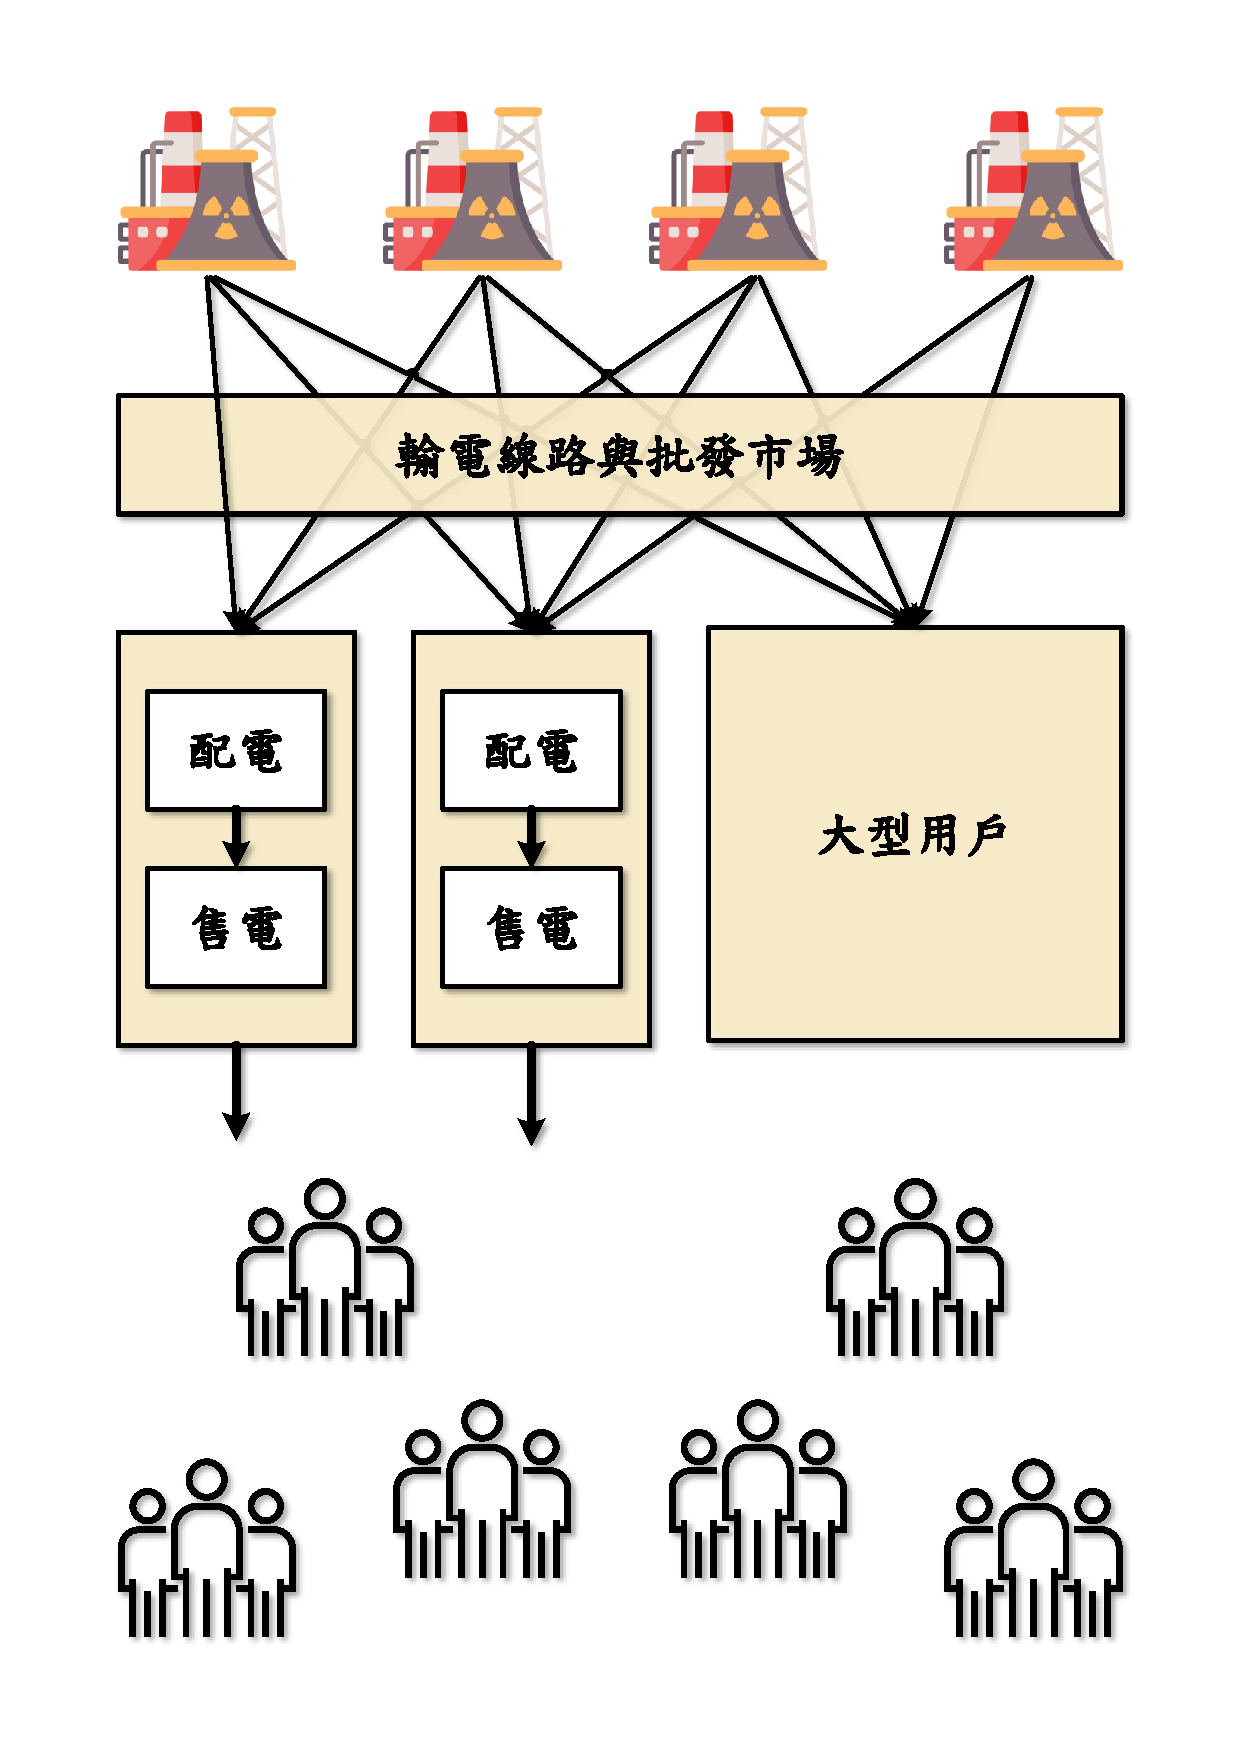
\includegraphics[width=\textwidth]{Power Wholesale Market}
    \caption[批發競爭]{批發競爭}
  \end{subfigure}
  \hfill
  \begin{subfigure}[d]{0.475\textwidth}
    \centering
    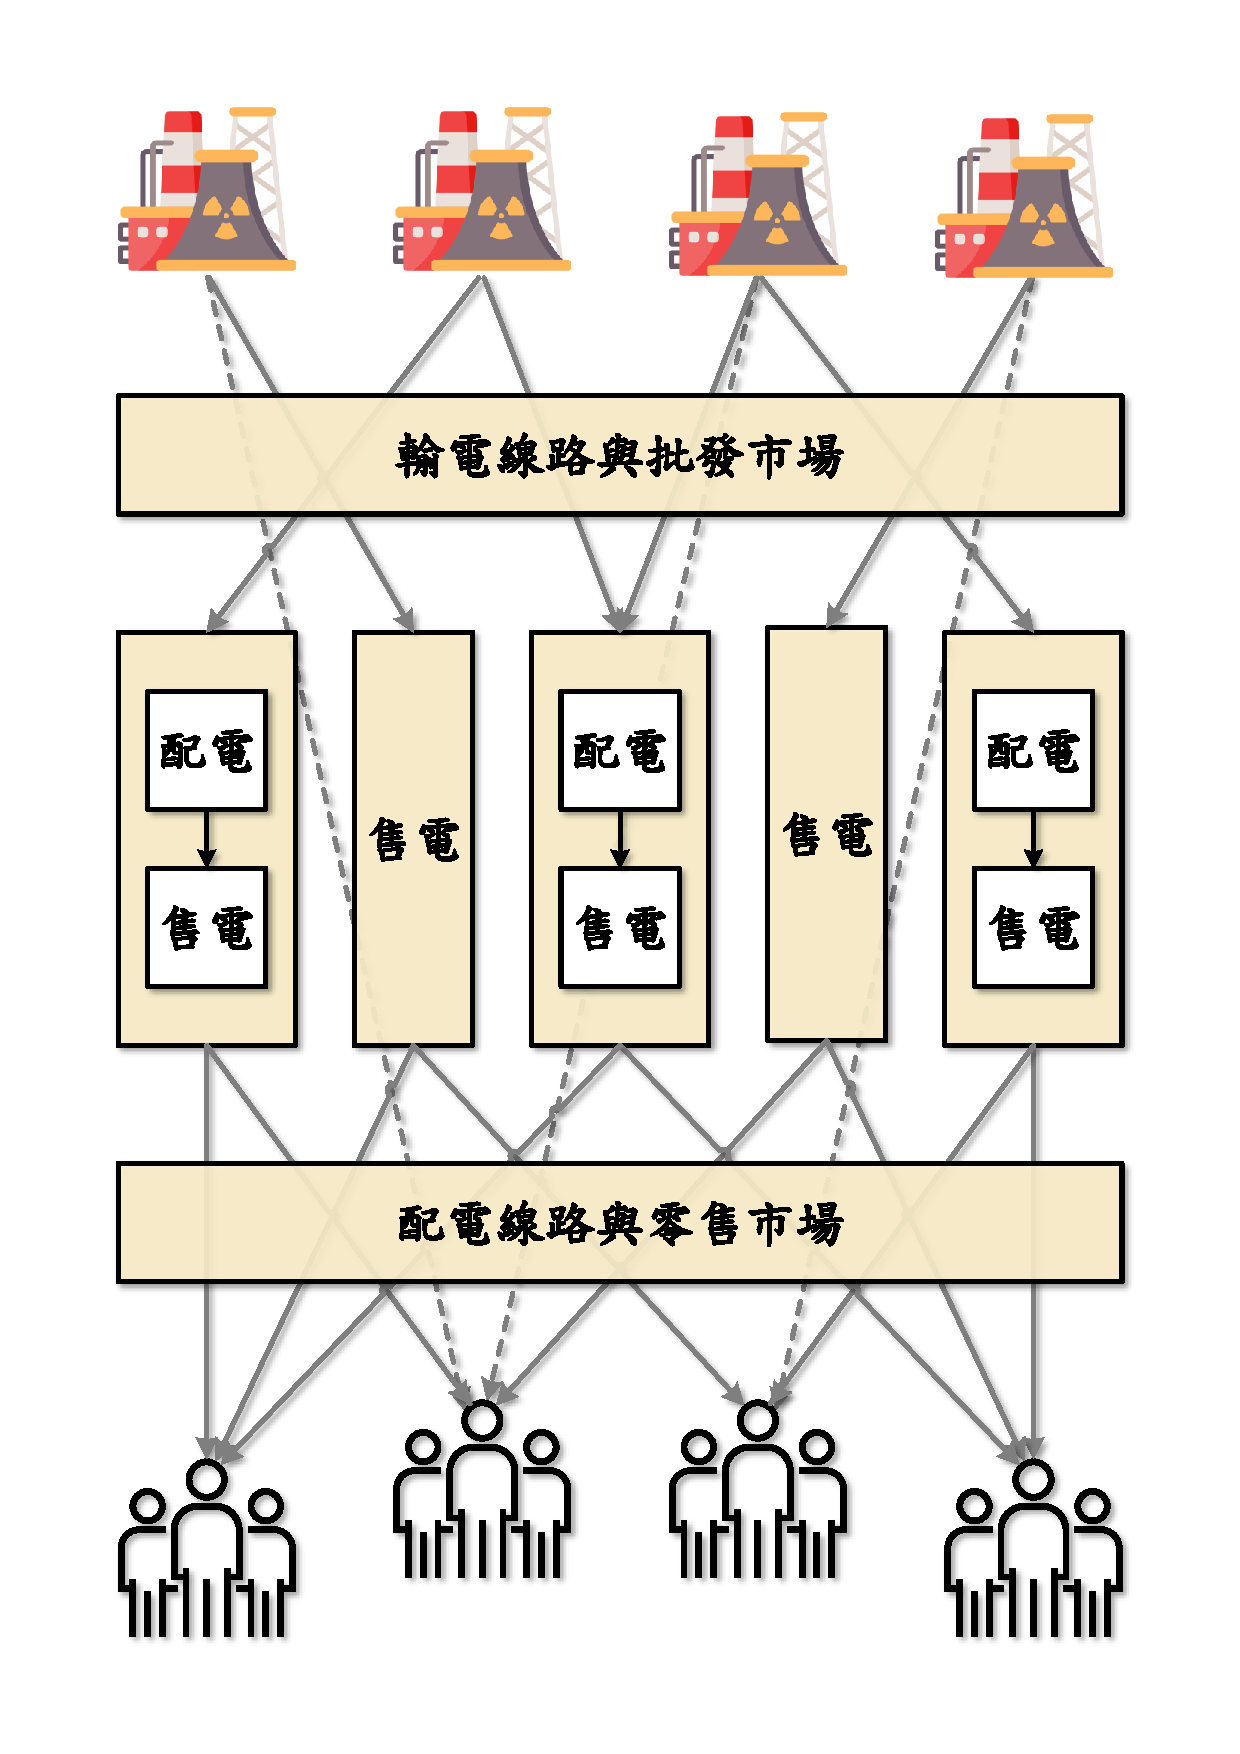
\includegraphics[width=\textwidth]{Power Retail Market}
    \caption[零售競爭]{零售競爭}
  \end{subfigure}
  \hfill
  \caption[常見電力市場架構]{常見電力市場架構}
  \label{figure: Power Markets}
\end{figure}

國際上電力市場的發展歷程,主要可以將電力市場分成垂直壟斷、單一買方、批發競爭及零售競爭等四個主要架構,如圖 \ref{figure: Power Markets} 所示 \cite{wang2015powermarket}。在獨佔電力市場中,由一家獨佔電力機構將上下游所有的發電、輸電、配電與售電業務進行垂直整合;而在自由電力市場中,則將上下游所有的發電、輸電、配電與售電業務水平分割成能夠獨立運作的機構 \cite{shahidehpour2003market},這些機構可能為:

\begin{itemize}
  \item \textbf{能源供應商(Generation Company, GENCO)}:電力市場中的供給端,調度可支配的發電機組生產能源,並根據簽訂的售電合約或電力拍賣進行出售。可以藉由調度發電機組和選擇不同交易方式來調整自身收益狀況。
  \item \textbf{電力使用者(Customer)}:電力市場中的需求端,獨佔電力市場中只能任由垂直整合綜合電業的電力公司制定電價進行交易,自由電力市場中可以自由選擇實惠的能源供應商簽約。通常根據規模可以分為大型用戶和個體用戶,大型用戶可以買賣電力,個體用戶僅能進行電力消費。
  \item \textbf{電力調度中心(Independent System Operator, ISO)}:負責制定市場運作規則、發電調度控制、維持系統安全,並以絕對中立的方式提供使用者進行交易。
\end{itemize}

\subsubsection{市場交易方式}

綜合目前世界上已實施電業自由化之各國的電力買賣方式,依據交易地點的分散與否,可以將自由化電力市場的交易方式分成以下三種 \cite{li2005strategic}:

\begin{itemize}
  \item \textbf{雙邊合約模式(Bilateral Contract Model)}:由供給端的能源供應商與需求端的電力使用者雙方直接簽訂交易合約,明定在特定時間內所願意交易的價格與數量,由電力調度所負責制定合約規範並在運作過程中檢驗供電品質。此模式下的供需雙方擁有較多選擇,但可能存在資訊不對等的狀況。
  \item \textbf{電力池模式(PoolCo Model)}:供給端的能源供應商與需求端的電力使用者必須向公正的電力交易場所(Power Exchange, PX)提出電力需求與競標價格,電力交易場所將依據雙方提供的資訊訂定市場結清價格(Market-Clearing Price)並告知買賣雙方進行交易。此模式下的供需雙方沒有太多選擇,但集中的協調、調度與定價流程有利於市場競爭。
  \item \textbf{混合型模式(Hybrid Model)}:結合了雙邊合約模式與電力池模式,供給端的能源供應商和需求端的電力使用者可以直接簽訂交易合約,也可以向電力交易所提出電力需求與競標價格,並從中選擇對自己較為有利的交易方式。此模式下既保留了一定的公平性,亦提供了相當程度的選擇。
\end{itemize}

其中,採用電力池模式或混合型模式的電力市場,皆需要透過電力交易場所(Power Exchange, PX)進行競標。目前根據電力調度中心與電力交易場所排程運作的時間,自由電力市場可以分成長期的期貨市場(Future Market)與短期的現貨市場(Spot Market)。電力期貨市場可以進行跨幅提前數週、數月甚至數年的電力交易,以避免未來可能的價格波動;電力現貨市場包括了日前市場(Day-Ahead Market)、日內市場(Intra-Day Market)與即時市場(Real-Time Market),其中又以日前市場最為常見。

在日前市場中,電力調度中心將於調度能源的前一天在電力交易場所公告預測的電力需求、電力最高價格、電力最低價格與競標重複一次所需時間…等相關交易資料,市場參與者必須在限定時間內提交可供調度的電力供給與競標價格,最後自最低的價格開始進行調度直至滿足前一日預測的電力需求為止。

\subsection{風機功率模型}

風力發電的原理,是風推動風機轉動葉片後,透過齒輪箱提升轉速後經由發電機進行發電,其中涉及了一系列風能、機械能與電能的轉換過程。本研究中採用風力發電機組的標準功率曲線作為風機模型,用以將風速轉換為對應的風能。風速與功率的對應關係一般以分段函數表示如方程式 \eqref{equation: Wind Power Model} 所示:

\begin{Equation}\label{equation: Wind Power Model}
  p_{wt}(v) = \left\{
  \begin{array}{cl}
    \displaystyle p_r \cdot \frac{v^{3} - v_{in}^{3}}{v_{r}^{3} - v_{in}^{3}} & ,~ {v}_{in} < v < v_r \\[18pt]
    p_r & ,~ v_r \leq v < v_{out} \\[18pt]
    0 & ,~ \text{otherwise}
  \end{array}\right.
\end{Equation}

其中,$P_{wt}(v)$ 為風力發電機組在風速為 $v$ 時所輸出的功率;$p_r$ 為風力發電機組的額定功率,又稱為裝置容量(capacity),亦即風力發電機組所能輸出的最大功率;$v_{in}$ 為風力發電機組的啟動風速,又稱為切入風速(cut-in speed),當風速大於啟動風速才開始運轉;$v_{out}$ 為風力發電機組的停機風速,又稱為切出風速(cut-out speed),當風速大於停機風速時會因安全考量停止自動運轉;$v_r$ 為風力發電機組的額定風速(rated speed)。

方程式 \eqref{equation: Wind Power Model} 表示:當風力發電機組的輸入風速大於啟動風速時,風力發電機組開始運轉,並根據不同的輸入風速產生相對應的電能,當風速達到額定風速時將以額定輸出功率運轉,當風速超過停機風速時,為保護葉片而停止輸出功率。

\subsection{電動汽車電池}

電動汽車係透過電池儲能的輸出推動馬達來行駛,為使電動汽車參與虛擬電廠進行電力市場交易,需要針對電動汽車電池原理進行了解。

\subsubsection{電池設備概述}

儲能電池設備透過電池內部的化學反應進行能量的釋放與儲存,一般儲能電池用於在緊急斷電狀況下及時供電或在用電尖峰時刻穩定電力系統,而電動汽車儲能電池為了推動馬達,還需要具備能夠長時間輸出一定大小電流。儲能電池設備主要由電池管理系統、交流/直流雙向轉換器與電池組所構成 \cite{qian2010high}。

其中車用電池管理系統需要針對電池充電狀況(State of Charge, SOC)與電池健康狀況(State of Health, SOH)進行評估與建模;交流/直流雙向轉換器與充電座進行能量轉移,用於將電池輸出的直流電轉換為交流電或將交流充電座輸入的交流電轉換為直流電;電池組則由多個電池串聯組成,電動汽車主要採用二次電池作為動力來源,約略可以分為鉛酸電池、鎳鎘電池、鎳氫電池與鋰離子電池,表 \ref{table: EV Battery} 為常見二次電池的特性比較 \cite{hsu2009evbattery},目前由於鋰電池相較其他電池而言具有較大的電流輸出與安全性,因此目前電動汽車廠商多針對鋰電池進行研究與推行車款。

\begin{table}[htp]
  \centering
  \caption[常見二次電池的特性比較]{常見二次電池的特性比較}
  \begin{tabular*}{\textwidth}{lccccc}
    \toprule
     & \textbf{鉛酸電池} & \textbf{聶鎘電池} & \textbf{鎳氫電池} & \textbf{鋰錳電池} & \textbf{磷酸鋰電池} \\
    \midrule
    \textbf{工作電壓} (V) & $2$ & $1.2$ & $1.2$ & $3.7$ & $3.3$ \\
    \textbf{體積能量密度} (Wh/L) & $100$ & $150$ & $250$ & $285$ & $270$ \\
    \textbf{重量能量密度} (Wh/Kg) & $30$ & $60$ & $80$ & $110$ & $120$ \\
    \textbf{電池功率密度} (Wh/Kg) & $300$ & $150$ & $800$ & $400$ & $2000$ \\
    \textbf{循環壽命} (次) & $400$ & $500$ & $500$ & $> 500$ & $> 2000$ \\
    \textbf{能量效率} (\%) & $60\%$ & $75\%$  & $70\%$ & $90\%$ & $95\%$ \\
    \textbf{安全性} & 佳 & 佳 & 佳 & 尚可 & 優 \\
    \textbf{充電時間} & 長 & 短 & 中 & 中 & 短 \\
    \textbf{記憶效應} & 無 & 大 & 小 & 無 & 無 \\
    \textbf{環保問題} & 有 & 有 & 無 & 無 & 無 \\
    \bottomrule
  \end{tabular*}
  \label{table: EV Battery}
\end{table}

\subsubsection{電池充電方法}

電池壽命除了會隨循環使用次數增加而降低之外,亦受到電池的充電與放電方式影響,採用適合的充電方法對於保護電池十分重要,常見的基本充電方法有定電壓充電法(Constant Voltage Charge)、定電流充電法(Constant Current Charge)與脈衝充電法(Pulsed Charge)。其中定電壓充電法為最普遍的充電方式,但存在無法確切估計充電時間且充電初期電流較大的問題;定電流充電法根據充電時間與電池容量設定電流值,但並未考慮初始電量狀態,充電效率不高且在高電壓時電池溫度會急遽上升;脈衝充電法透過週期性電流進行充電,能適當調整電流大小並有時間予以緩衝。

電池使用過程中,輸出容量佔其額定容量 $E$($\text{Ah}$)的百分比稱為放電深度(Depth of Discharge, DoD),定義如方程式 \eqref{equation: Depth of Discharge} 所示,其中 $E$($\text{Ah}$)為電池額定容量,$E_{r}$($\text{Ah}$) 為電池剩餘電量。

\begin{equation}\label{equation: Depth of Discharge}
  \text{DoD}~(\%) = \frac{E - E_{r}}{E} \times 100 \%
\end{equation}

不同的放電深度會影響二次電池的充電放電循環次數 \cite{dogger2010characterization},因此一般會將電池壽命以其生命週期內的放電次數函數 $L(\text{DoD})$ 進行表示。 

\subsection{模型預測控制}

模型預測控制(Model Predictive Contrl, MPC),又稱為移動時域控制(Moving Horizon Contrl, MHC)或後退時域控制(Receding Horizon Control, RHC),是近年來自動控制領域中被廣泛應用於工業上的一種反饋控制策略 \cite{richalet1978model}。透過模型預測控制可以在每一個時刻都根據當前的資訊求解有限時域內的最佳化問題,因此能夠更加精準地進行系統的控制,相較於傳統的控制方法更適合用於複雜系統中。

\subsubsection{模型預測控制基本原理}

模型預測控制的基本原理如圖 \ref{figure: Model Predictive Contrl} 所示,左側為過去時刻的狀態,右側為未來時刻的狀態。模型預測控制法在當前時刻 $k$ 時, 根據過去時刻的狀態進行最佳化求解並預測未來輸出結果,在下一時刻時取前一次所得到的預測結果並捨棄其餘結果,並反覆進行此過程。

\begin{figure}[htbp]
  \centering
  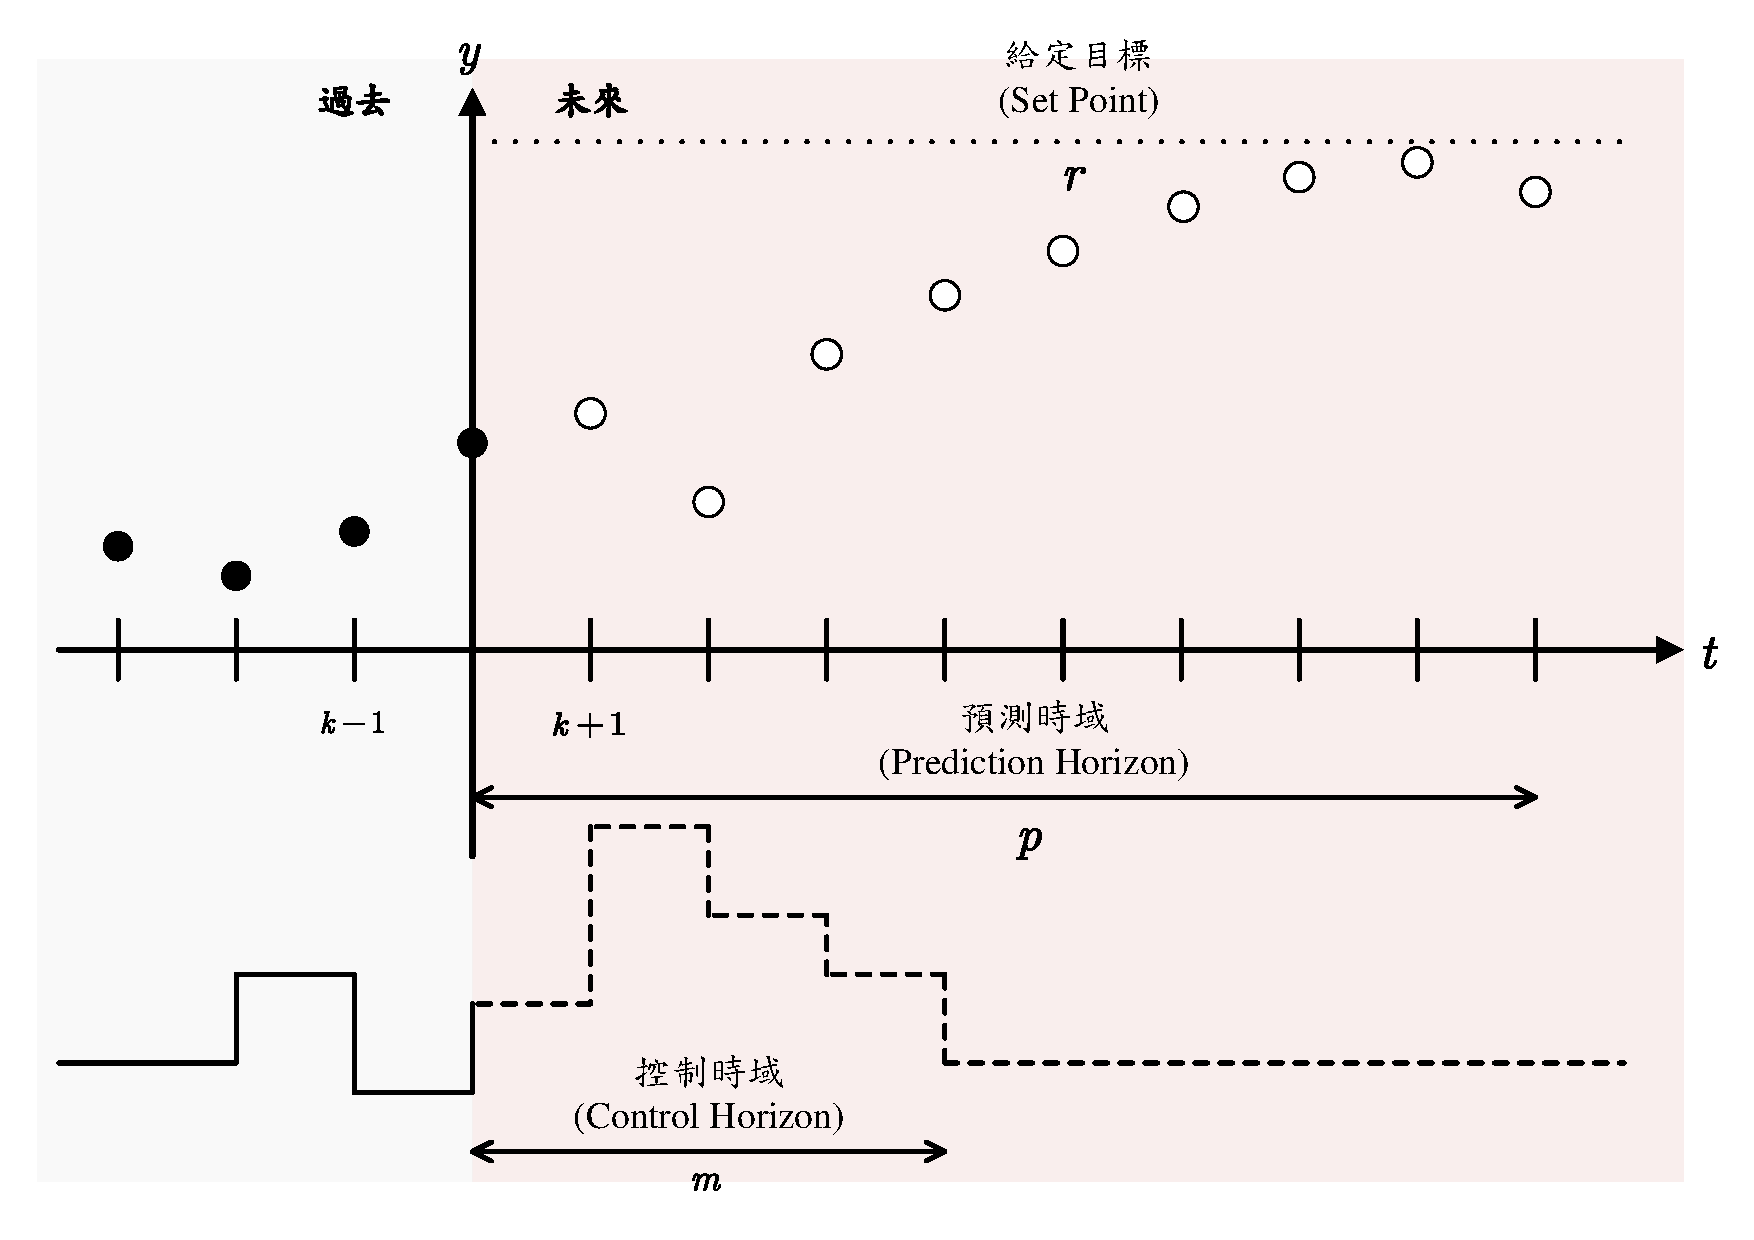
\includegraphics[width=0.8\textwidth]{Model Predictive Control}
  \caption{模型預測控制基本原理}
  \label{figure: Model Predictive Contrl}
\end{figure}

一般可以將模型預測控制的實現步驟依次拆解為模型預測、滾動優化與反饋校正三個部分:

\begin{enumerate}
  \item \textbf{模型預測}:此部分為模型預測控制的基礎,根據系統的當前狀態和預測模型,對未來行為與輸出進行預測,其中預測模型通常以狀態方程式的形式表示
  \item \textbf{滾動優化}:模型預測控制在未來的有限時域內,透過某一性能指標的參考值進行未來控制決策的最佳化,其中下一時刻的只使用當前所得到控制變數來進行最佳化,並且反覆進行這個過程
  \item \textbf{反饋校正}:由於採用有限時域進行預測,封閉的控制系統中同時存在外部干擾與內部模型不確定性,每一時刻都需要檢測當前系統實際的狀況,並根據實際數值與預測結果之間的誤差進行校正
\end{enumerate}

\subsubsection{模型預測控制數學模型}

考慮線性離散時間系統的狀態空間模型如方程式 \eqref{equation: Linear Discrete System State Model} 所示:

\begin{equation}\label{equation: Linear Discrete System State Model}
  \begin{aligned}
    x(k + 1)    &= Ax(k) + B_{u} u(k) + B_{d} d(k) \\
    y_{c} (k)   &= C_{c} x(k)                      \\
    y_{b} (k)   &= C_{b} x(k)
  \end{aligned}
\end{equation}

其中,$k$ 為當前時刻,$x(k) \in \mathbb{R}^{n}$ 為狀態變數,$u(k) \in \mathbb{R}^{n}$ 為控制變數,$y_{c}(k) \in \mathbb{R}^{n}$ 和 $y_{b} (k) \in \mathbb{R}^{n}$ 為被控輸出變數與約束輸出變數,$d(k) \in \mathbb{R}^{n}$ 為可以被測量的外部干擾變數,而 $A, B_{u}, B_{d}, C_{c}$ 和 $C_{b}$ 為對應維度大小的系統矩陣。方程式 \eqref{equation: Linear Discrete System State Model} 表示下一時刻的狀態變數 $x(k + 1)$ 可以由當前時刻的狀態變數 $x(k)$ 和控制變數 $u(k)$ 進行預測,且輸出變數為狀態變數與控制變數的函數。

為減少與消除靜態誤差,考慮方程式 \eqref{equation: Linear Discrete System State Model Argument} 所示的增量模型。

\begin{equation}\label{equation: Linear Discrete System State Model Argument}
  \begin{aligned}
    \Delta x(k + 1)     &= A \Delta x(k) + B_{u} \Delta u(k) + B_{d} \Delta d(k) \\
    y_{c} (k)           &= C_{c} \Delta x(k) + y_{c} (k-1)                       \\
    y_{b} (k)           &= C_{b} \Delta x(k) + y_{b} (k-1)
  \end{aligned}
\end{equation}

其中,$\Delta x(k) = x(k) - x(k-1)$ 為狀態增量,$\Delta u(k) = u(k) - u(k-1)$ 為控制輸入增量,$\Delta d(k) = d(k) - d(k-1)$ 為被測量的外部干擾增量。

假設控制時域為 $m$,預測時域為 $p$ 且 $m \leq p$,則控制系統未來 $p$ 步被控輸出和約束輸出的預測方程式可以表示為方程式 \eqref{equation: Future p Steps Predicitve Model} 所示。

\begin{equation}\label{equation: Future p Steps Predicitve Model}
  \begin{aligned}
    Y_{p, c} (k+1 | k) = S_{x, c} \Delta x(k) + I_{c} y_{c} (k) + S_{u, c} \Delta U(k) + S_{d, c} \Delta d(k) \\
    Y_{p, b} (k+1 | k) = S_{x, b} \Delta x(k) + I_{b} y_{b} (k) + S_{u, b} \Delta U(k) + S_{d, b} \Delta d(k)
  \end{aligned}
\end{equation}

其中,$S_{x, c}, I_{c}, S_{u, c}, S_{x, b}, I_{b}, S_{u, b}, S_{d, b}$ 為相應維度大小的系統預測矩陣。該控制系統的控制目標為使得被控輸入 $y_{c}$ 滿足給定參考輸入 $r$,同時系統的控制量、控制增量與輸出量須滿足方程式 \eqref{equation: Predicitve Model Constraints} 所示的約束條件。

\begin{equation}\label{equation: Predicitve Model Constraints}
  \begin{aligned}
    u_{\min} (k) \leq u(k) \leq u_{\max} (k) &, \forall k \geq 0 \\
    y_{\min} (k) \leq y_{b}(k) \leq y_{\max} (k) &, \forall k \geq 0 \\
    \Delta u_{\min} (k) \leq \Delta u(k) \leq \Delta u_{\max} (k) &, \forall k \geq 0
  \end{aligned}
\end{equation}

假設控制系統的全部狀態都可以被測量得到,在當前時刻 $k$ 以測量值 $x(k), y_{c}(k), y_{b}(k)$ 作為預測系統未來動態預測的初始條件,根據預測控制的基本原理,可以將模型預測控制表示為方程式 \eqref{equation: MPC Programming Problem} 所示的最佳化模型。

\begin{equation}\label{equation: MPC Programming Problem}
  \begin{aligned}
    \min_{\Delta U(k)} \qquad & J(x(k), \Delta U(k)) \\
    \text{s.t.}        \qquad & \Delta x(k+i+1 | k) = A\Delta x(k+i|k) + B_{u} \Delta u(k+i) + B_{d} \Delta d(k + i) \\
                              & \Delta x(k|k) = \Delta x(k) \\
                              & y_{c} (k+i|k) = C_{c} \Delta x(k+i|k) + y_{c} (k+i-1|k), i \geq 1 \\
                              & y_{c} (k|k) = y_{c}(k) \\
                              & y_{b} (k+i|k) = C_{b} \Delta x(k+i|k) + y_{c} (k+i-1|k) \\
                              & y_{b} (k|k) = y_{b}(k) \\
                              & u_{\min} (k+i) \leq u(k+i) \leq u_{\max} (k+i) \\
                              & y_{\min} (k+i) \leq y_{b}(k+i) \leq y_{\max} (k+i) \\
                              & \Delta u_{\min} (k+i) \leq \Delta u(k+i) \leq \Delta u_{\max} (k+i)
  \end{aligned}
\end{equation}

其中,$J(x(k), \Delta U(k)) = \norm{\Gamma_{y} (Y_{p, c}(k+1|k)-R(k+1))}^2 + \norm{\Gamma_{u} \Delta U(k)}^2$。在上述最佳化模型中,$R(k+1)$ 是給定的控制輸出參考向量,控制量增量向量 $\Delta U(k)$ 為約束最佳化問題的獨立變數,而 $\Gamma_{y}$ 和 $\Gamma_{u}$ 是對稱正定加權矩陣,定義如方程式 \eqref{equation: Weight Matrix} 所示。

\begin{equation}\label{equation: Weight Matrix}
  \begin{aligned}
    \Gamma_{y} &= \text{diag} \{ \Gamma_{y, 1}, \Gamma_{y, 2}, \cdots, \Gamma_{y, p} \}_{p \times p} \\
    \Gamma_{u} &= \text{diag} \{ \Gamma_{u, 1}, \Gamma_{u, 2}, \cdots, \Gamma_{u, m} \}_{m \times m} \\
  \end{aligned}
\end{equation}

其中 $\Gamma_{y, i}$ 是在預測 $i$ 時刻對被控輸出誤差的加權因子,其值越大表示期望對應的預測控制輸出越接近給定的參考輸入;而 $\Gamma_{u, i}$ 是在預測 $i$ 時刻對控制增量的加權因子,其值越大表示期望對應的控制動作變化越小。在進行控制器設計時,需要調節這兩個參數來滿足系統控制要求。

\section{小結}

本章扼要地描述了研究流程,並針對研究流程中的風力發電預測與收益模型分析部分所會使用到的方法與理論進行說明與介紹,包括了小波時頻轉換、時間序列預測、支持向量迴歸和模型預測控制…等。後續章節將根據本章所介紹的理論與方法進行模型建構以及案例分析,並詳述其內容與概念。
% !TeX root = ../main.tex

\chapter{模型建構}

本章為模型建構,在介紹完研究過程中所會使用到的理論與方法後,需要將這些理論與方法根據應用情境建立模型並實際用於計算。在這一章節中,將闡述風速預測部分的時間序列預測模型建構流程,以及收益分析部分的風力電場與電動汽車等效模型,並於下一章節中將模型實際應用於案例中進行分析。

\section{風力電場發電預測}

\subsection{時間序列預測建模流程}

自迴歸移動平均模型 $\text{ARIMA}(p, d, q)$ 的建構流程如圖 \ref{figure: Time Series Model Flow} 所示。在取得時間序列資料後,需要先進行平穩性檢驗,若時間序列不具備平穩性則必須差分 $d$ 次進行平穩化;接著繪製其 ACF 與 PACF 圖形並由其特徵初步決定其自迴歸項 $p$ 與移動平均項 $q$ 之值;初步階數選定之後透過 AIC 與 BIC 進行評價並選出最適模型以進行時間序列預測。

\begin{figure}[htbp]
  \centering
  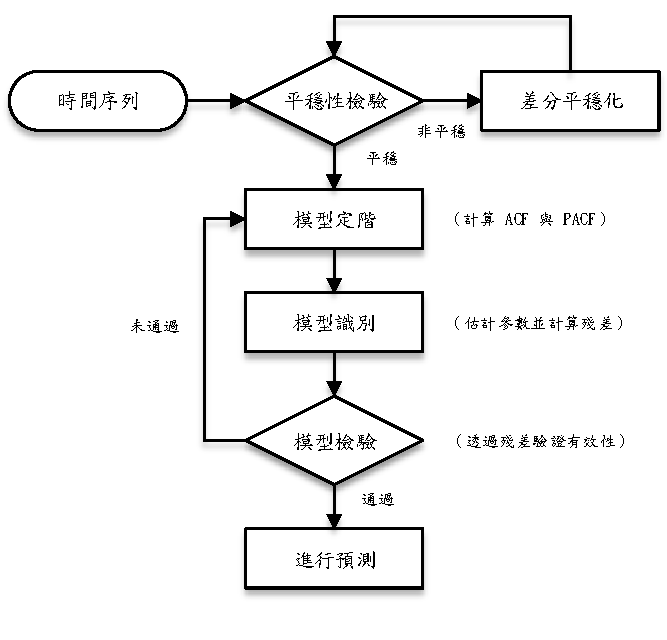
\includegraphics{time_series_model_flow}
  \caption{時間序列預測建模流程}
  \label{figure: Time Series Model Flow}
\end{figure}

\subsection{支持向量迴歸建模流程}

支持向量迴歸模型的建構流程如圖 \ref{figure: Support Vector Regression Flow} 所示,在取得資料之後,會先將資料拆分為訓練集合 (training set) 與測試集合 (testing set),並選擇適當的核函數與特徵參數進行模型訓練,在計算出表現最佳的模型參數後,使用測試集合進行評價並選出最適模型進行預測。

\begin{figure}[htbp]
  \centering
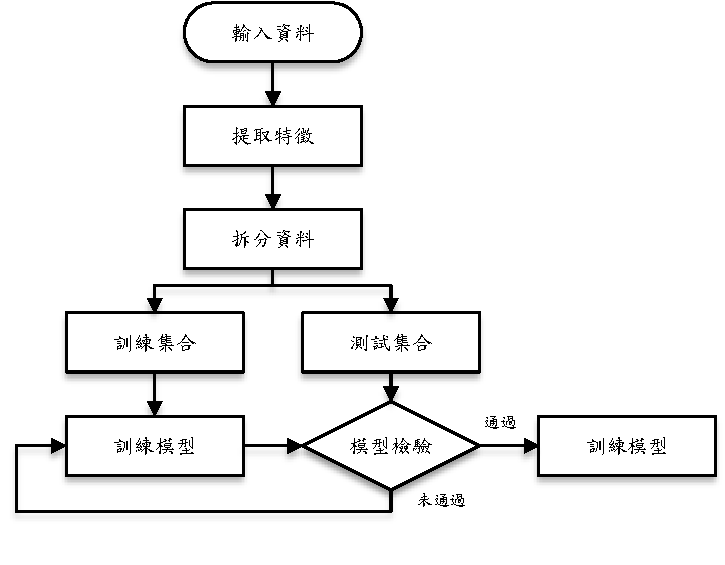
\includegraphics{support_vector_regression_model_flow}
  \caption{支持向量迴歸建模流程}
  \label{figure: Support Vector Regression Flow}
\end{figure}

\subsection{組合預測模型建模流程}

常見的組合預測模型是將預測的結果進行線性組合,根據加權方式可以再分為採用權重相等的簡單平均組合以及依據情境調整權重的變動權重組合,前者雖簡潔較易於計算但無法有效突出不同模型的優勢,後者則需要嘗試不同組合來尋找最佳的權重分配;本研究擬採用小波分解將原始時間序列進行解構,根據分解後各分量的特性分別採取較佳的預測方法後再將結果進行組合,組合時不需進行權重的分配。本研究將採用下述兩種組合預測模型,並比較其預測能力:
%
\begin{itemize}
  \item \textbf{一般等權組合預測模型} \\
        \begin{equation}\label{equation: Normal Combine Model}
          \hat{y}(t) = \frac{1}{2} \hat{y}_{\text{ARIMA}} (t) + \frac{1}{2} \hat{y}_{\text{SVR}} (t)
        \end{equation}
  \item \textbf{小波分解組合預測模型} \\
        \begin{equation}\label{equation: Wavelet Combine Model}
          \hat{y}(t) = \hat{A}_{2} (t) + \hat{D}_{1} (t) + \hat{D}_{2} (t)
        \end{equation}
\end{itemize}
%
上述模型的建構流程分別如圖 \ref{figure: Linear Combine Model Flow} 和圖 \ref{figure: Wavelet Combine Model Flow} 所示。一般等權組合預測模型即為分別使用單一預測模型進行預測後,將預測結果使用同樣的權重進行線性組合;小波分解組合預測模型則是將時間序列,透過離散小波轉換分解為近似分量與細節分量,並分別採用 ARIMA 模型與 SVR 模型進行預測,再將預測結果進行整合。

\begin{figure}[htbp]
  \centering
  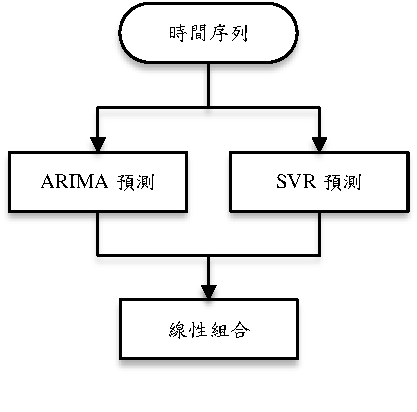
\includegraphics{linear_combine_model_flow}
  \caption[一般等權組合預測模型建模流程]{一般等權組合預測模型建模流程}
  \label{figure: Linear Combine Model Flow}
\end{figure}

\begin{figure}[htbp]
  \centering
  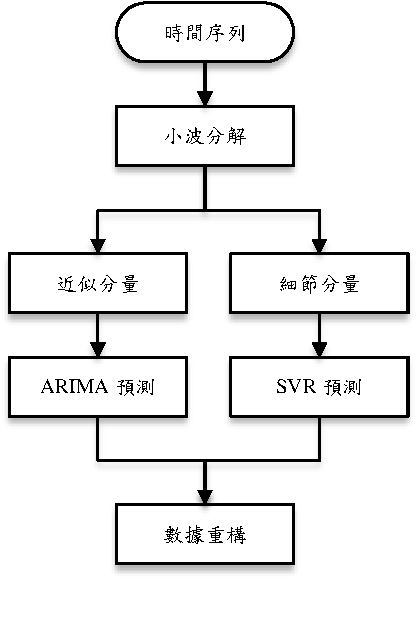
\includegraphics{wavelet_combine_model_flow}
  \caption[小波分解組合預測模型建模流程]{小波分解組合預測模型建模流程}
  \label{figure: Wavelet Combine Model Flow}
\end{figure}

\section{虛擬電廠收益分析}

\subsection{虛擬電廠架構概述}

本文採用的虛擬電廠 (Virtual Power Plant, VPP) 架構如圖 \ref{figure: Virtual Power Plant Model} 所示,由風力電場 (Wind Farm, WF)、電動汽車 (Electric Vehicle, EV) 組成,分別透過發電與儲能來參與電力市場 (Electric Market, EM)。

\begin{figure}[htbp]
  \centering
  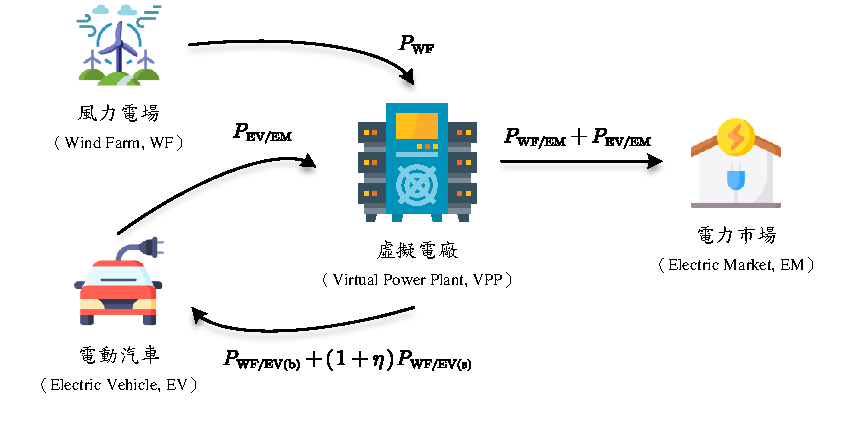
\includegraphics{virtual_power_plant_model}
  \caption{整合風力電場與電動汽車的虛擬電廠模型}
  \label{figure: Virtual Power Plant Model}
\end{figure}

由於風力電場發電數量預測仰賴於短期風速之預測結果,本研究考慮虛擬電廠參與日前市場交易之情境:在日前市場中,電網營運業者會在調度能源的前一天,提交電力需求並在競價後與發電業者簽署合約,規定發電業者提供約定的發電數量,如果與合約中保證的發電數量存在偏差則需要予以賠償;因此虛擬電廠作為發電業者,必須在第 $(t-1)$ 日提交價格資訊,並保證在第 $t$ 日的每個時段提供一定的發電數量。

對於虛擬電廠中的風力電場而言,需要在第 $(t-1)$ 日根據歷史風速資訊預測第 $t$ 日的風速,評估發電數量後給出在第 $t$ 日願意參與虛擬電廠的電動汽車數量與決定所需的最佳儲存數量,以此在日前市場中提出最有利的競標價格,並在滿足合約內容的前提下,根據實際的發電數量滾動式地持續更新其供應計畫。

對於虛擬電廠中的電動汽車而言,由於參與儲能後會增加電動汽車電池的充電放電次數,進而導致電池壽命減少,因此需要對電動汽車車主進行補償,以增加其參與虛擬電廠的意願。考量參與虛擬電廠的電動汽車無法如傳統儲能設備那般直接計算運轉成本,在本研究中不採用直接給予金錢的補償支付,而是無償地向電動汽車提供充電額度,亦即利用批發電價與零售電價之間差額的所得營收,換取電動汽車作為儲能設備的動機。

\subsection{風力電場等效模型}

若已知特定風力機組 $M$ 的額定功率曲線,則可以透過某一時段 $t$ 的風速資料 $v(t)$ 確定該時段所對應的風力機組發電狀況,如方程式 \eqref{equation: Wine Turbine Power} 所示。
%
\begin{equation}\label{equation: Wine Turbine Power}
  P_{\text{wt},M} (t) = P_{\text{wt},M} (v (t))
\end{equation}
%
假定一風力電場 (Wind Farm) 內設置有風力發電機組 $M_{1}, M_{2}, \dots, M_{k}$,則在當天某一時段 $t$ 的預測發電總量可以表示如方程式 \eqref{equation: Wind Farm Power} 所示。
%
\begin{equation}\label{equation: Wind Farm Power}
  P_{\text{WF}}(t) = \sum_{i = 1}^{k} P_{\text{wt}, M_i} (t)
\end{equation}
% %
% 在本文的模擬情況中,預測風速資料將以每一小時作為時間間隔,為了方便進行運算,最終將以向量形式表示在時間範圍內該風力電場不同單位時段的預測發電總量,用以參與電力市場作為日前市場的投標資訊,如方程式 \eqref{equation: Wind Farm Power Vector} 所示。
% %
% \begin{equation}\label{equation: Wind Farm Power Vector}
%   \boldsymbol{P_{\text{WF}}} = [ P_{\text{WF}}(1) P_{\text{WF}}(2) P_{\text{WF}}(3) \cdots P_{\text{WF}}(N) ]^{\top}
% \end{equation}

\subsection{電動汽車等效模型}

電動汽車透過儲存電能到電池中來參與虛擬電廠的電力市場交易,對於每一輛電動汽車 $V$ 而言都有其對應的儲存容量,假定一電動汽車 (Electric Vehicle) 集合中設置有電動汽車 $V_{1}, V_{2}, \dots, V_{h}$,則在當天某一時段 $t$ 的儲存容量上限可以表示如方程式 \eqref{equation: Electriv Vehicle Set Power} 所示。
%
\begin{equation}\label{equation: Electriv Vehicle Set Power}
  S_{\text{EV}}(t) = \sum_{i = 1}^{h} S_{V_i} (t)
\end{equation}
% %
% 在本文的模擬情況中,為配合以每一小時作為時間間隔的預測風速資料進行建模運算,同樣將以向量形式表示在時間範圍內,所有電動汽車在不同單位時段的儲存容量上限,如方程式 \eqref{equation: Electric Vehicle Power Vector} 所示。
% %
% \begin{equation}\label{equation: Electric Vehicle Power Vector}
%   \boldsymbol{S_{\text{EV}}} = [ S_{\text{EV}}(1) S_{\text{EV}}(2) S_{\text{EV}}(3) \cdots S_{\text{EV}}(N) ]^{\top}
% \end{equation}

\subsection{電力市場收益模型}

\subsubsection{日前市場調度}

根據前述架構,虛擬電廠將根據風力電場的預測發電數量,調度電動汽車進行儲存能量來參與電力市場交易,並透過規劃求解計算虛擬電廠的最大收益,其最佳化模型可由方程式 \eqref{equation: Virual Power Plant Profit Model} 表示。
%
\begin{subequations}\label{equation: Virual Power Plant Profit Model}
  \begin{alignat}{2}
    \max        \qquad & \sum_{t = 1}^{N} p_{e}(t) \times [P_{\text{WF/EM}}(t) + P_{\text{EV/EM}}(t)] \label{subequation: Virual Power Plant Profit Model 1} \\
    \text{s.t.} \qquad & P_{\text{WF/EM}}(t) + P_{\text{WF/EV(b)}}(t) + (1 + \eta)P_{\text{WF/EV(s)}}(t) = P_{\text{WF}}(t) \label{subequation: Virual Power Plant Profit Model 2} \\
                       & \sum_{i=1}^{t-1} \left[ P_{\text{WF/EV(s)}}(i) - P_{\text{EV/EM}}(i) \right] + P_{\text{WF/EV(s)}}(t) \leq P_{\text{ST}}(t) \label{subequation: Virual Power Plant Profit Model 3} \\
                       & \sum_{i=1}^{t-1} \left[ P_{\text{WF/EV(s)}}(i) - P_{\text{EV/EM}}(i) \right] - P_{\text{EV/EM}}(t) \geq 0 \label{subequation: Virual Power Plant Profit Model 4} \\
                       & P_{\text{WF/EV(b)}}(t) \geq \sigma P_{\text{ST}}(t) \label{subequation: Virual Power Plant Profit Model 5} \\
                       & 0 \leq P_{\text{ST}}(t) + P_{\text{WF/EV(b)}}(t) \leq S_{\text{EV}}(t) \label{subequation: Virual Power Plant Profit Model 6} \\
                       & P_{\text{WF/EM}}(t), P_{\text{WF/EV(s)}}(t),  P_{\text{WF/EV(b)}}(t),P_{\text{EV/EM}}(t) \geq 0 \label{subequation: Virual Power Plant Profit Model 7}
  \end{alignat}
\end{subequations}
%
其中,$p_{e} (t)$ 為虛擬電廠在電力交易市場中的販售電力價格;$P_{\text{WF/EM}}(t)$ 為風力電場輸送至電力交易市場中進行販售的電力數量;$P_{\text{WF/EV(s)}}(t)$ 為風力電場輸送至電動汽車電池中進行儲存的電力數量;$P_{\text{WF/EV(b)}}(t)$ 為風力電場輸送至電動汽車電池中作為補償的電力數量;$P_{\text{EV/EM}}(t)$ 為電動汽車輸送至電力交易市場中進行販售的電力數量;$P_{\text{ST}}(t)$ 為虛擬電廠需要的電力儲存容量;$\eta$ 為電動汽車電池在充放電過程的能量轉換損耗比例 ($\eta \in [0, 1]$)。

% 目標函數說明
式 \eqref{subequation: Virual Power Plant Profit Model 1} 為目標函數,為了使得電動汽車與風力電場參與虛擬電廠進行電力市場交易的收益最大,其中虛擬電廠販售電力的收入,可以表示為虛擬電廠電力市場中的販售電力價格 $p_{e} (t)$ 個別和虛擬電廠輸送到電力市場的電力數量 $P_{WF/EM}(t)$ 與電動汽車輸送到電力市場的電力數量 $P_{EV/EM}(t)$ 進行乘積後的總和。

% 限制條件說明
式 \eqref{subequation: Virual Power Plant Profit Model 2} 為限制條件,表示風力電場在 $t$ 時段的預測發電數量 $P_{\text{WF}}(t)$ 可以分配 $P_{\text{WF/EM}}(t)$ 輸送至電力交易市場中進行販售、$P_{\text{WF/EV(b)}}(t)$ 輸送至電動汽車電池中作為補償、$P_{\text{WF/EV(s)}}(t)$ 輸送至電動汽車電池中進行儲存,其中考慮到電動汽車電池在充放電過程中存在能源轉換耗損,每一單位的電力數量在充放電時會損失 $\eta$ 單位的電力數量 ($\eta \in [0, 1]$)。

式 \eqref{subequation: Virual Power Plant Profit Model 3} 為限制條件,表示在 $t$ 時段的電動汽車電池在過去所儲存的 (現在所擁有的) 電力數量 $\sum_{i=1}^{t-1} \left[ P_{\text{WF/EV(s)}}(i) - P_{\text{EV/EM}}(i) \right]$ 與該時段欲再儲存的電力數量 $P_{\text{WF/EV(s)}}(t)$ 不得超過電動汽車的可用儲存容量 $P_{\text{ST}}(t)$。

式 \eqref{subequation: Virual Power Plant Profit Model 4} 為限制條件,表示在 $t$ 時段的電動汽車電池能夠輸送至電力交易市場中進行販售的電力數量 $P_{\text{EV/EM}}(t)$ 不得超過電動汽車電池過去時段所累積的 (現在所擁有的) 儲存電量 $\sum_{i=1}^{t-1} \left[ P_{\text{WF/EV(s)}}(i) - P_{\text{EV/EM}}(i) \right]$。

式 \eqref{subequation: Virual Power Plant Profit Model 5} 為限制條件,表示風力電場輸送至電動汽車電池中作為補償的電力數量 $P_{\text{WF/EV(b)}}(t)$
需大於虛擬電廠需要的儲存容量 $P_{\text{ST}}(t)$ 的一定比例 $\sigma \in [0, 1]$。

式 \eqref{subequation: Virual Power Plant Profit Model 6} 為限制條件,表示在 $t$ 時段虛擬電廠需要的儲存容量 $P_{\text{ST}}(t)$ 與風力電場輸送至電動汽車電池中作為補償的電力數量 $P_{\text{WF/EV(b)}}(t)$ 必須小於所有電動汽車在該時段的儲存容量總量 $S_{\text{EV}}(t)$。

式 \eqref{subequation: Virual Power Plant Profit Model 7} 為非負限制式,表示在任一時段的電力傳輸過程中,風力電場輸送至電力交易市場中進行販售的電力數量 $P_{\text{WF/EM}}(t)$、風力電場輸送至電動汽車電池中進行儲存的電力數量 $P_{\text{WF/EV(s)}}(t)$、風力電場輸送至電動汽車電池中作為補償的電力數量 $P_{\text{WF/EV(b)}}(t)$ 和 電動汽車輸送至電力交易市場中進行販售的電力數量 $P_{\text{EV/EM}}(t)$ 需滿足本文所提出之虛擬電廠架構的傳輸方向。

\subsubsection{模型預測控制}

藉由模型預測控制方法,可以利用過去的規劃結果建立系統預測模型,並實時更新系統資訊進行規劃求解。在移動時域中,考慮虛擬電廠在參與電力市場交易時,發電數量可能與投標時的保證數量存在偏差,而必須予以賠償的情況,因此在模型預測控制方法中的最佳化模型可由方程式 \eqref{equation: Virual Power Plant Profit MPC Model} 表示,並在交易當天透過在每個時段更新系統資訊計算時段最佳解進而求得整體最佳解。
%
\begin{subequations}\label{equation: Virual Power Plant Profit MPC Model}
  \begin{alignat}{2}
    \max        \qquad & \sum_{t = k}^{N} p_{e}(t) \times [P_{\text{WF/EM}}'(t) + P_{\text{EV/EM}}'(t) - A(t) - B(t)] \label{subequation: Virual Power Plant Profit MPC Model 1} \\
    \text{s.t.} \qquad & P_{\text{WF/EM}}'(t) + P_{\text{WF/EV(b)}}'(t) + (1 + \eta)P_{\text{WF/EV(s)}}'(t) = P_{\text{WF}}'(t) \label{subequation: Virual Power Plant Profit MPC Model 2} \\
                       & \sum_{i=1}^{t-1} \left[ P_{\text{WF/EV(s)}}'(i) - P_{\text{EV/EM}}'(i) \right] + P_{\text{WF/EV(s)}}'(t) \leq P_{\text{ST}}(n) \label{subequation: Virual Power Plant Profit MPC Model 3} \\
                       & \sum_{i=1}^{t-1} \left[ P_{\text{WF/EV(s)}}'(i) - P_{\text{EV/EM}}'(i) \right] - P_{\text{EV/EM}}'(t) \geq 0 \label{subequation: Virual Power Plant Profit MPC Model 4} \\
                       & P_{\text{WF/EV(b)}}'(t) \geq \sigma P_{\text{ST}}'(t) \label{subequation: Virual Power Plant Profit MPC Model 5} \\
                       & 0 \leq P_{\text{ST}}'(t) + P_{\text{WF/EV(b)}}'(t) \leq S_{\text{EV}}'(t) \label{subequation: Virual Power Plant Profit MPC Model 6} \\
                       & [P_{\text{WF/EM}}(t) + P_{\text{EV/EM}}(t)] - [P_{\text{WF/EM}}'(t) + P_{\text{EV/EM}}'(t)] \leq A(t) \label{subequation: Virual Power Plant Profit MPC Model 7} \\
                       & [P_{\text{WF/EM}}'(t) + P_{\text{EV/EM}}'(t)] - [P_{\text{WF/EM}}(t) + P_{\text{EV/EM}}(t)] \leq B(t) \label{subequation: Virual Power Plant Profit MPC Model 8} \\
                       & P_{\text{WF/EM}}'(t), P_{\text{WF/EV(s)}}'(t),  P_{\text{WF/EV(b)}}'(t),P_{\text{EV/EM}}'(t),A(t),B(t) \geq 0 \label{subequation: Virual Power Plant Profit MPC Model 9}
  \end{alignat}
\end{subequations}
%
其中,$p_{e} (t)$ 為虛擬電廠在電力交易市場中的販售電力價格;$A(t)$ 和 $B(t)$ 表示缺額電力數量與超出電力數量;$P_{\text{WF/EM}}'(t)$ 為更新後風力電場輸送至電力交易市場中進行販售的電力數量;$P_{\text{WF/EV(s)}}'(t)$ 為更新後風力電場輸送至電動汽車電池中進行儲存的電力數量;$P_{\text{WF/EV(b)}}'(t)$ 為更新後風力電場輸送至電動汽車電池中作為補償的電力數量;$P_{\text{EV/EM}}'(t)$ 為更新後電動汽車輸送至電力交易市場中進行販售的電力數量;$P_{\text{ST}}'(t)$ 為更新後虛擬電廠所需要的電力儲存容量;$\eta$ 為電動汽車電池在充放電過程的能源轉換損耗比率 ($\eta \in [0, 1]$)。

% 目標函數說明
式 \eqref{subequation: Virual Power Plant Profit MPC Model 1} 為目標函數,為使電動汽車與風力電場參與虛擬電廠進行電力市場交易的收益最大,其中虛擬電廠販售電力收入可以表示為虛擬電廠販售給電網的電力價格 $p_{e} (t)$ 個別和虛擬電廠傳輸到電網的電力數量 $P_{WF/EM}(t)$ 與電動汽車傳輸到電網的電力數量 $P_{EV/EM}(t)$ 乘積的總和。

% 限制條件說明
式 \eqref{subequation: Virual Power Plant Profit MPC Model 2} 為限制條件,表示風力電場在 $t$ 時段更新後的預測發電數量 $P_{\text{WF/EM}}'(t)$ 可以分配 $P_{\text{WF/EM}}'(t)$ 輸送至電力交易市場中進行販售、$P_{\text{WF/EV(b)}}'(t)$ 輸送至電動汽車電池中作為補償、$P_{\text{WF/EV(s)}}'(t)$ 輸送至電動汽車電池中進行儲存,其中考慮了電動汽車電池在充放電過程中存在能源轉換耗損,每一單位的電力數量在充放電時會損失 $\eta$ 單位的電力數量。

式 \eqref{subequation: Virual Power Plant Profit MPC Model 3} 為限制條件,表示在 $t$ 時段更新後的電動汽車電池在過去所儲存的 (現在所擁有的) 電力電量 $\sum_{i=1}^{t-1} \left[ P_{\text{WF/EV(s)}}'(i) - P_{\text{EV/EM}}'(i) \right]$ 與該時段欲存入的儲存電量 $P_{\text{WF/EV(s)}}'(t)$ 不得超過電動汽車的可用儲存容量 $P_{\text{ST}}'(t)$。

式 \eqref{subequation: Virual Power Plant Profit MPC Model 4} 為限制條件,表示在 $t$ 時段更新後的電動汽車電池能夠輸送至電力交易市場中進行販售的電力數量 $P_{\text{EV/EM}}'(t)$ 不得超過電動汽車電池過去時段所累積的 (現在所擁有的) 儲存電量 $\sum_{i=1}^{t-1} \left[ P_{\text{WF/EV(s)}}'(i) - P_{\text{EV/EM}}'(i) \right]$。

式 \eqref{subequation: Virual Power Plant Profit MPC Model 5} 為限制條件,表示更新後的風力電場輸送至電動汽車電池中作為補償的電力數量 $P_{\text{WF/EV(b)}}'(t)$ 需大於虛擬電廠需要的儲存容量 $P_{\text{ST}}'(t)$ 的一定比例 $\sigma \in [0, 1]$。

式 \eqref{subequation: Virual Power Plant Profit MPC Model 6} 為限制條件,表示在 $t$ 時段更新後的虛擬電廠需要的儲存容量 $P_{\text{ST}}'(t)$ 與風力電場輸送至電動汽車電池中作為補償的電力數量 $P_{\text{WF/EV(b)}}'(t)$ 必須小於所有電動汽車在該時段的儲存容量總量 $S_{\text{EV}}'(t)$。

式 \eqref{subequation: Virual Power Plant Profit MPC Model 7} 為限制條件,表示缺額電力數量 $A(t)$ 必須大於合約電力數量 $[P_{\text{WF/EM}}(t) + P_{\text{EV/EM}}(t)]$ 與實際電力數量 $[P_{\text{WF/EM}}'(t) + P_{\text{EV/EM}}'(t)]$ 之差值。

式 \eqref{subequation: Virual Power Plant Profit MPC Model 8} 為限制條件,表示超出電力數量 $B(t)$ 必須大於實際電力數量 $[P_{\text{WF/EM}}'(t) + P_{\text{EV/EM}}'(t)]$ 與合約電力數量 $[P_{\text{WF/EM}}(t) + P_{\text{EV/EM}}(t)]$ 之差值。

式 \eqref{subequation: Virual Power Plant Profit MPC Model 9} 為非負限制式,表示在更新後任一時段的電力傳輸過程中,風力電場輸送至電力交易市場中進行販售的電力數量 $P_{\text{WF/EM}}'(t)$、風力電場輸送至電動汽車電池中進行儲存的電力數量 $P_{\text{WF/EV(s)}}'(t)$、風力電場輸送至電動汽車電池中作為補償的電力數量 $P_{\text{WF/EV(b)}}'(t)$ 和電動汽車輸送至電力交易市場中進行販售的電力數量 $P_{\text{EV/EM}}'(t)$ 需滿足本文所提出之虛擬電廠架構的傳輸方向。

\subsection{預測控制求解流程}

模型預測控制求解流程如圖 \ref{figure: Model Predictive Control Flow} 所示,在取得當前時段 $t$ 的系統資訊後,預測輸出結果並進行最佳化求解,若未完成控制時域內之預測,則求解控制變數並進行下一時段的系統調度,如此反覆進行。

\begin{figure}[htbp]
  \centering
  \includegraphics{model_predictive_control_flow}
  \caption{模型預測控制求解流程}
  \label{figure: Model Predictive Control Flow}
\end{figure}

\section{小結}

本章說明了研究的模型建構部分,包括風力電場發電預測部分中的 ARIMA 預測模型、SVR 預測模型和小波分解組合預測模型的建構流程,以及收益分析中風力電場與電動汽車的等效模型、虛擬電廠最佳化收益模型以及考慮了移動時域的模型預測控制求解流程。在下一章節中將實際使用我國\uline{澎湖}地區\uline{東吉島} (DONGJIDAO) 測站的歷史風速資料進行發電預測並進行收益分析。

% !TeX root = ../main.tex

\chapter{案例分析}

本章為案例分析,第一部分進行風速預測分析,並計算不同預測模型的誤差結果來比較模型的預測能力,第二部分進行收益結果分析,並透過控制參數比較在不同情況下之收益結果。

\section{模擬情境概述}

% 設備概述
本研究模擬與分析所使用的電腦,其硬體設備採用 Intel® Core™ i7 處理器,記憶體共 24 GB,運行 Microsoft Windows 10 作業系統。並使用 MathWorks 公司出品的商業數學軟體 MATrix LABoratory (MATLAB) 與以程式語言 Python 為基礎的數值分析與統計模型套件進行模擬與分析之程式開發。

% 風力資料
關於歷史風速資料與模擬場址的選擇,考量我國\uline{澎湖}、\uline{金門}與\uline{馬祖}地區由於孤立於臺灣本島的電力傳輸系統之外,較適合作為含風力發電與電動汽車的的虛擬電廠參與電力市場交易的模擬案例。本文使用\uline{東吉島}(DONGJIDAO)測站(北緯 $23^\circ 15' 32''$,東經 $119^\circ 39'34''$)於 2018 年的風速資料,並根據表 \ref{table: Taiwan Wind Farm Data} 所示的我國風力發電場址資料,假設模型中的風力電場由八座 Enercon E40/600 Model 風力發電機組與四座 Enercon E44/900 Model 風力發電機組所構成。

% 電力價格
收益分析部分的電力價格將採用因應不同用電狀況與發電情況所制定的時間電價(Time of Use Price, TOU),這樣一來虛擬電廠在參與電力市場時,可以根據時間電價制定發電計畫,用以平衡波動並獲取較大收益,比如在離峰時段儲存電能至電動汽車,而在尖峰時段販售電力。但由於我國智慧電錶尚未完全普及,因此未能有效針對不同時段制定電價,而是以季節區分並制定大略峰值時段電價,本文將採用表 \ref{table: Electric Price} 所示的臺灣電力公司非夏季兩段式電價進行收益計算 \cite{taipower2018price}。

\begin{table}[htp]
  \centering
  \caption[臺灣電力公司非夏季兩段式電價]{臺灣電力公司非夏季的兩段式電價 \cite{taipower2018price}}
  \begin{tabular}{cr}
    \toprule
    \textbf{時間}   & \textbf{電價(元/度)}   \\
    \midrule
    00:00 - 07:30   & NT \$1.73                \\
    07:30 - 22:30   & NT \$4.23                \\
    22:30 - 24:00   & NT \$1.73                \\
    \bottomrule
  \end{tabular}
  \label{table: Electric Price}
\end{table}

% 電動汽車

\section{風速預測分析}

\subsection{歷史風速概述}

此處採用\uline{東吉島}(DONGJIDAO)測站於 $2018$ 年間風速跨度較大的十二月份歷史風速資料進行風力電場短期發電預測示範計算,取該月份中前二十九日共 $696$ 個小時的歷史風速作為觀測資料,預測最後二日共 $48$ 小時的短期風速,並比較不同預測模型的誤差結果。在後續內容中,將選擇預測能力較佳的模型進行全年預測以作為收益分析中參與虛擬電廠的風力電場發電數量。

圖 \ref{figure: Historial Wind Speed} 為根據\uline{東吉島}(DONGJIDAO)測站 $2018$ 年十二月份的歷史風速資料所繪製的原始風速時間序列,顯示在該月份中所測得之歷史風速有較大幅度的變化,且初步判斷該時間序列具備趨勢性故為非平穩時間序列。

\begin{figure}[htbp]
  \centering
  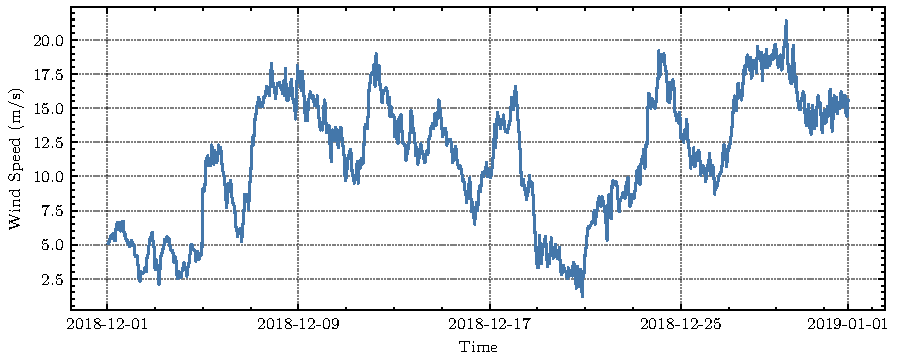
\includegraphics[width=\textwidth]{Historial Wind Speed}
  \caption{原始風速時間序列}
  \label{figure: Historial Wind Speed}
\end{figure}

由於採用圖形檢驗法觀察時間序列平穩性可能根據觀察者不同而存在主觀性差異,本文採用 Augmented Dickey-Fuller 檢定進行單根檢驗,其平穩性檢驗結果如表 \ref{table: Raw Time Series ADF Result} 所示,由於 ADF 檢驗統計量並不同時小於在 $99\%$、$95\%$ 與 $90\%$ 信賴區間下的 ADF 臨界檢驗值,因此原始風速資料時間序列為非平穩時間序列。

\begin{table}[htbp]
  \centering
  \caption[原始風速時間序列 ADF 檢定結果]{原始風速時間序列 ADF 檢定結果}
  \begin{tabular}{lr}
    \toprule
    \textbf{檢驗統計量} & \textbf{數值}     \\
    \midrule
    Test Statistic          & $-3.217446$   \\
    p-value                 & $1.8997 \times 10^{-2}$    \\
    Critical Value ($1\%$)  & $-3.439377$   \\
    Critical Value ($5\%$)  & $-2.865524$   \\
    Critical Value ($10\%$) & $-2.568891$   \\
    \bottomrule
  \end{tabular}
  \label{table: Raw Time Series ADF Result}
\end{table}

\subsection{單一預測模型}

\subsubsection{ARIMA 模型}

由於 ARIMA 模型的概念在於透過歷史資料的自相關性進行未來結果的預測,為使採用樣本時間序列所得到的擬合曲線在未來短期時間內延續既有型態,所採用的時間序列須具備平穩性。由前述內容已知原始風速時間序列為非平穩時間序列,因此需反覆計算時間序列中當前時刻與前一時刻的差值來取得其差分後的平穩時間序列。

\begin{figure}[htbp]
  \centering
  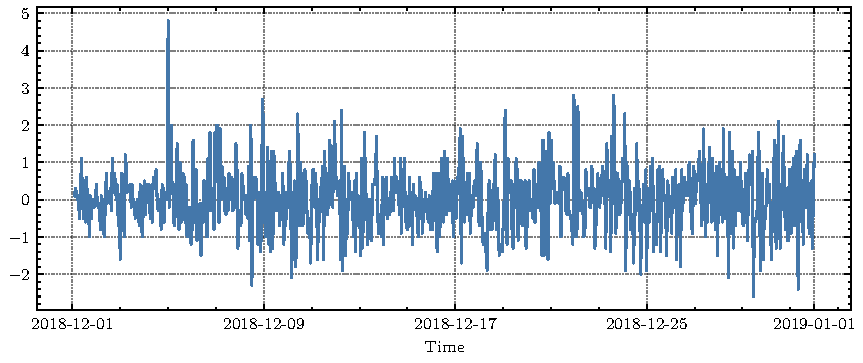
\includegraphics[width=\textwidth]{Difference Wind Speed}
  \caption{差分風速時間序列}
  \label{figure: Difference Wind Speed}
\end{figure}

將原始風速時間序列進行一階差分後所得到的差分風速時間序列如圖 \ref{figure: Difference Wind Speed} 所示,由圖形可初步判斷該時間序列已具備平穩性。為避免觀察者不同而存在的主觀性差異,採用 Augmented Dickey-Fuller 檢定進行單根檢驗的平穩性檢驗結果如表 \ref{table: Difference Time Series ADF Result} 所示,其中 ADF 檢驗統計量已同時小於在 $99\%$、$95\%$ 與 $90\%$ 信賴區間下的 ADF 臨界檢驗值,且 p-value 已十分接近零,因此該差分風速時間序列已為平穩時間序列。

\begin{table}[htbp]
  \centering
  \caption[差分風速時間序列 ADF 檢定結果]{差分風速時間序列 ADF 檢定結果}
  \begin{tabular}{lr}
    \toprule
    \textbf{檢驗統計量} & \textbf{數值}     \\
    \midrule
    Test Statistic          & $-21.391265$  \\
    p-value                 & $5.817483 \times 10^{-27}$    \\
    Critical Value ($1\%$)  & $-3.439206$   \\
    Critical Value ($5\%$)  & $-2.865448$   \\
    Critical Value ($10\%$) & $-2.568851$   \\
    \bottomrule
  \end{tabular}
  \label{table: Difference Time Series ADF Result}
\end{table}

圖 \ref{figure: Difference Wind Speed ACF}  和圖 \ref{figure: Difference Wind Speed PACF} 分別為差分時間序列的自相關係數函數(Autocorrelation Function, ACF)圖與非自相關係數函數(Partial Autocorrelation Function, PACF)圖,由圖形可知其自相關係數函數在延遲項 Lag 值為 $2$ 時落入信賴區間中,其偏自相關係數函數在延遲項 Lag 值為 $3$ 時落入信賴區間中,據此可認定其時間序列具備平穩性並可大致識別其模型可採用 $\text{ARIMA} (2, 1, 3)$。

\begin{figure}[htbp]
  \centering
  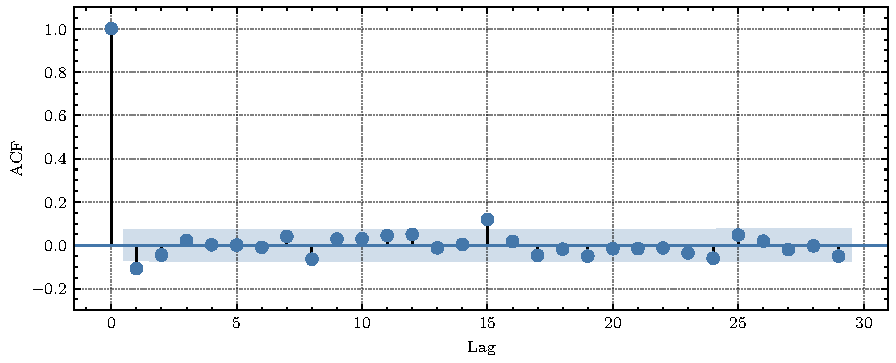
\includegraphics[width=\textwidth]{Difference Wind Speed ACF}
  \caption{差分時間序列自相關係數函數(ACF)圖}
  \label{figure: Difference Wind Speed ACF}
\end{figure}

\begin{figure}[htbp]
  \centering
  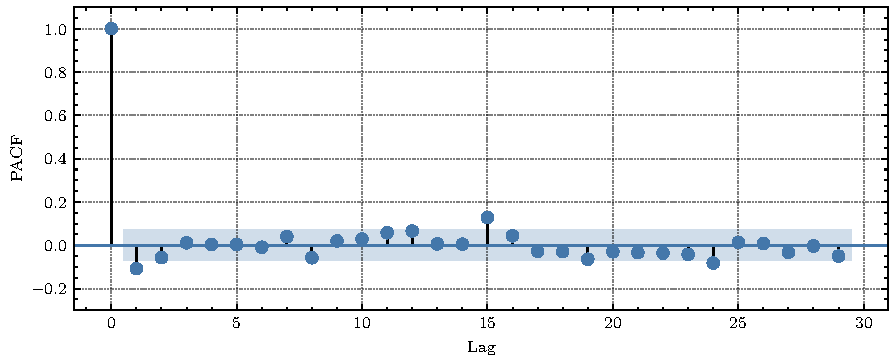
\includegraphics[width=\textwidth]{Difference Wind Speed PACF}
  \caption{差分時間序列偏自相關係數函數(PACF)圖}
  \label{figure: Difference Wind Speed PACF}
\end{figure}

透過自相關係數函數圖與偏自相關係數函數圖進行模型定階可能存在主觀性差異,通常會使用 AIC(Akaike's Information Criterion)及 BIC(Bayesian Information Criterion)作為評價模型優劣的指標,採用窮舉法擬合所有模型並選出具有較小 AIC 值的最適模型。表 \ref{table: Auto ARIMA Result} 為使用開放式源代碼套件 \texttt{pyramid} 所提供的 \texttt{auto\_arima()} 函數針對差分時間序列模型進行窮舉擬合所得到的結果,採用 AIC 值最小的 $\text{ARIMA} (2, 1, 0)$ 模型進行短期預測,預測結果如圖 \ref{figure: Wind Speed Prediction ARIMA} 所示。

\begin{table}[htbp]
  \centering
  \caption[差分風速時間序列 $\text{ARIMA}(p, d, q)$ 適配檢驗]{差分風速時間序列 $\text{ARIMA}(p, d, q)$ 適配檢驗}
  \begin{tabular}{cccc}
    \toprule
    \textbf{模型} & \textbf{AIC} & \textbf{BIC} & \textbf{Time} \\
    \midrule
    $\text{ARIMA}(1,1,1)$ & $1886.365$ & $1904.808$ & $0.229$ \si{s} \\
    $\text{ARIMA}(1,1,2)$ & $1886.528$ & $1909.581$ & $0.424$ \si{s} \\
    $\text{ARIMA}(1,1,3)$ & $1888.300$ & $1915.964$ & $0.404$ \si{s} \\
    $\text{ARIMA}(1,1,4)$ & $1890.242$ & $1922.517$ & $0.619$ \si{s} \\
    $\text{ARIMA}(2,1,0)$ & $1885.681$ & $1904.124$ & $0.087$ \si{s} \\
    $\text{ARIMA}(2,1,1)$ & $1887.588$ & $1910.641$ & $0.258$ \si{s} \\
    $\text{ARIMA}(2,1,2)$ & $1889.564$ & $1917.228$ & $0.165$ \si{s} \\
    $\text{ARIMA}(2,1,3)$ & $1890.281$ & $1922.556$ & $0.890$ \si{s} \\
    $\text{ARIMA}(3,1,0)$ & $1887.576$ & $1910.630$ & $0.110$ \si{s} \\
    $\text{ARIMA}(3,1,1)$ & $1889.572$ & $1917.236$ & $0.155$ \si{s} \\
    $\text{ARIMA}(3,1,2)$ & $1890.944$ & $1923.219$ & $0.955$ \si{s} \\
    $\text{ARIMA}(4,1,0)$ & $1889.565$ & $1917.229$ & $0.138$ \si{s} \\
    $\text{ARIMA}(4,1,1)$ & $1891.564$ & $1923.839$ & $0.184$ \si{s} \\
    \bottomrule
  \end{tabular}
  \label{table: Auto ARIMA Result}
\end{table}

\begin{figure}[htbp]
  \centering
  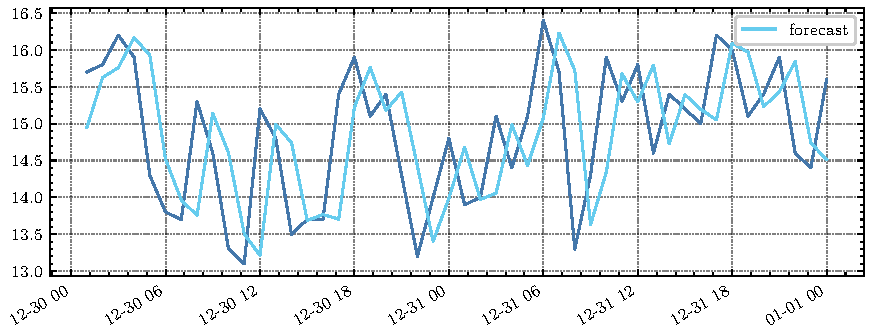
\includegraphics[width=\textwidth]{Wind Speed Prediction (ARIMA)}
  \caption{單一 ARIMA 模型短期風速預測結果}
  \label{figure: Wind Speed Prediction ARIMA}
\end{figure}

\subsubsection{SVR 模型}

基於支持向量迴歸模型進行時間序列預測時,在將歷史風速資料進行標準化後,採用時間間隔為 $1$ 單位的延遲,並選用高斯徑向核函數進行預測。使用開放式源代碼套件 \texttt{sklearn} 所提供的 \texttt{SVR()} 函數針對風速時間序列模型進行預測的結果如圖 \ref{figure: Wind Speed Prediction SVR} 所示。

\begin{figure}[htbp]
  \centering
  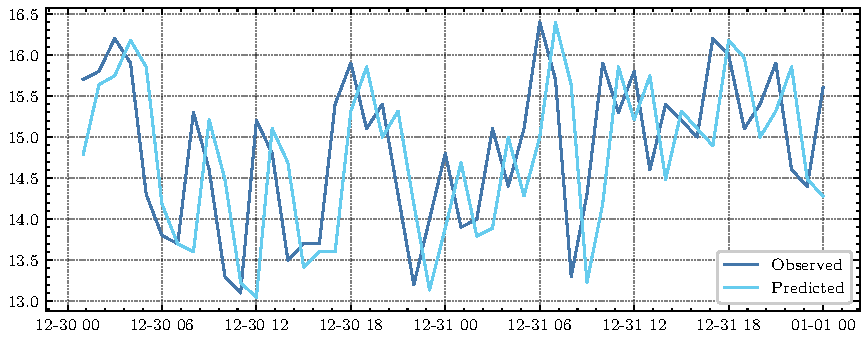
\includegraphics[width=\textwidth]{Wind Speed Prediction (SVR)}
  \caption{單一 SVR 模型短期風速預測結果}
  \label{figure: Wind Speed Prediction SVR}
\end{figure}

\subsection{組合預測模型}

\subsubsection{一般等權 ARIMA-SVR 組合模型}

本文採用的一般等權 ARIMA-SVR 組合模型如方程式 \eqref{equation: Normal Combine Model} 所示,即使用相等權重將前述單一預測模型中 ARIMA 模型與 SVR 模型的預測結果進行線性組合。根據單一 ARIMA 模型與單一 SVR 模型預測結果進行相等權重線性組合的預測結果如圖 \ref{figure: Wind Speed Prediction Linear} 所示。

\begin{figure}[htbp]
  \centering
  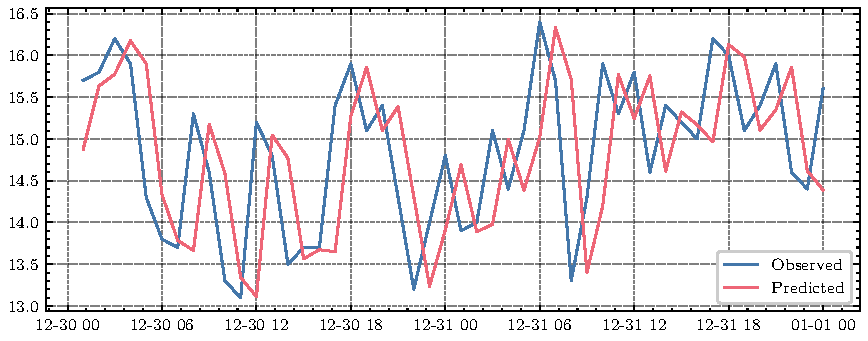
\includegraphics[width=\textwidth]{Wind Speed Prediction (Linear)}
  \caption{一般等權 ARIMA-SVR 組合模型短期風速預測結果}
  \label{figure: Wind Speed Prediction Linear}
\end{figure}

\subsubsection{小波分解 ARIMA-SVR 組合模型}

本文採用的小波分解 ARIMA-SVR 組合模型如方程式 \eqref{equation: Wavelet Combine Model} 所示,即將時間序列透過離散小波轉換分解為高頻部分(細節分量)與低頻部分(近似分量),並分別採用 ARIMA 模型預測與 SVR 模型預測,再將預測結果進行重構與整合。

針對時間序列採用較平滑且解析度較高的 Daubechies Wavelet 小波或 Symlet 小波進行分解較為合適。本文使用不同消失矩 $N$ 的 Daubechies Wavelet 小波將原始風速時間序列進行不同 層數的訊號分解後進行訊號重構所得到的誤差如表 \ref{table: Wavelet Reconstruction Error} 所示,顯示採用 db4 小波進行 $2$ 層的訊號分解能夠在訊號重構時產生較小的誤差。

\begin{table}[htp]
  \centering
  \caption[原始風速時間序列進行小波分解的重構誤差]{原始風速時間序列進行小波分解的重構誤差}
  \begin{tabular*}{0.65\textwidth}{lcccc}
    \toprule
    \textbf{分解層數} & $\text{db}_3$ \textbf{小波} & $\text{db}_4$ \textbf{小波} & $\text{db}_5$ \textbf{小波} & $\text{db}_6$ \textbf{小波} \\
    \midrule
    $2$ 層分解 & $2.8931$ & $1.1759$ & $4.2143$ & $3.2171$ \\
    $3$ 層分解 & $4.1932$ & $2.1486$ & $5.9631$ & $4.7622$ \\
    $4$ 層分解 & $4.3194$ & $3.0123$ & $7.3174$ & $5.4318$ \\
    \bottomrule
    & & & & ($\times 10^{-10}$)
  \end{tabular*}
  \label{table: Wavelet Reconstruction Error}
\end{table}

在使用開放式源代碼套件 \texttt{pywt} 所提供的 \texttt{wavedec()} 函數,選擇 db4 小波對原始風速時間序列進行 $2$ 層小波分解與重構後,可以得到如圖 \ref{figure: Approximated Component Level 2 (A2)} 所示反映整體趨勢的近似分量 $A1$,以及如圖 \ref{figure: Detailed Component Level 2 (D2)} 和圖 \ref{figure: Detailed Component Level 1 (D1)} 所示反映細小波動的細節分量 $D2$ 和 $D1$。

\begin{figure}[hbp]
  \centering
  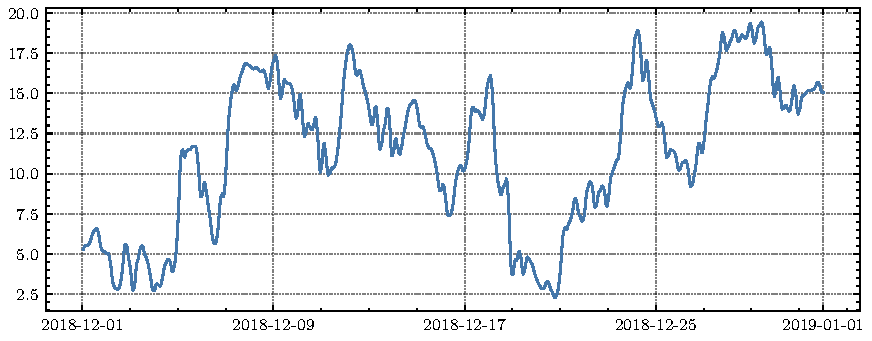
\includegraphics[width=\textwidth]{Approximated Component in Level 2 (A2)}
  \caption{原始風速時間序列進行小波分解的近似分量 $A2$}
  \label{figure: Approximated Component Level 2 (A2)}
  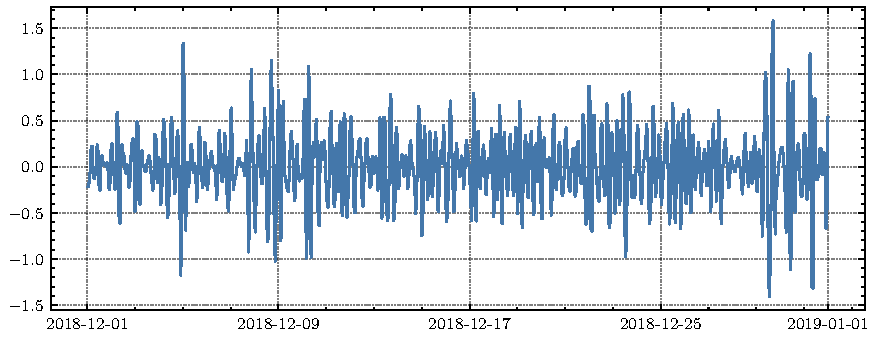
\includegraphics[width=\textwidth]{Detailed Component in Level 2 (D2)}
  \caption{原始風速時間序列進行小波分解的細節分量 $D2$}
  \label{figure: Detailed Component Level 2 (D2)}
  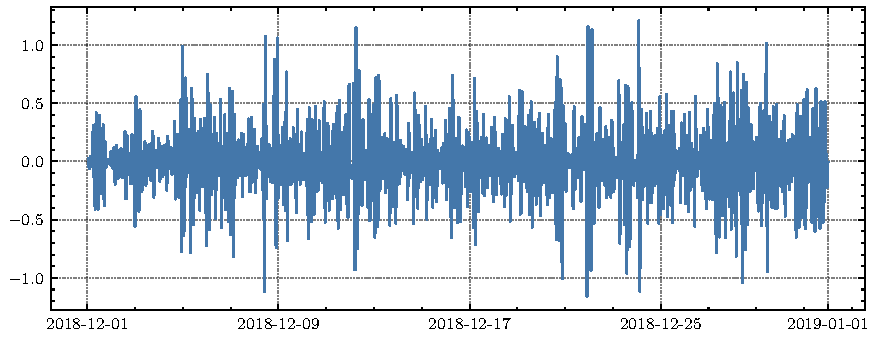
\includegraphics[width=\textwidth]{Detailed Component in Level 1 (D1)}
  \caption{原始風速時間序列進行小波分解的細節分量 $D1$}
  \label{figure: Detailed Component Level 1 (D1)}
\end{figure}

採用 Augmented Dickey-Fuller 檢定對原始風速時間序列經小波分解後所得到的細節分量 $D2$ 和 $D1$ 進行單根檢驗,其平穩性檢驗結果分別如表 \ref{table: D2 ADF Result} 和表 \ref{table: D1 ADF Result} 所示,其中 ADF 檢驗統計量皆已同時小於在 $99\%$、$95\%$ 與 $90\%$ 信賴區間下的 ADF 臨界檢驗值,且 p-value 已十分接近零,因此細節分量 $D2$ 和 $D1$ 皆為平穩時間序列。

\begin{table}[htbp]
  \centering
  \caption[原始風速時間序列 $D2$ 細節分量 ADF 檢定結果]{原始風速時間序列 $D2$ 細節分量 ADF 檢定結果}
  \begin{tabular}{lr}
    \toprule
    \textbf{檢驗統計量} & \textbf{數值}     \\
    \midrule
    Test Statistic          & $-13.40788$  \\
    p-value                 & $4.433267 \times 10^{-25}$    \\
    Critical Value ($1\%$)  & $-3.439427$   \\
    Critical Value ($5\%$)  & $-2.865446$   \\
    Critical Value ($10\%$) & $-2.568903$   \\
    \bottomrule
  \end{tabular}
  \label{table: D2 ADF Result}
\end{table}

\begin{table}[htbp]
  \centering
  \caption[原始風速時間序列 $D1$ 細節分量 ADF 檢定結果]{原始風速時間序列 $D1$ 細節分量 ADF 檢定結果}
  \begin{tabular}{lr}
    \toprule
    \textbf{檢驗統計量} & \textbf{數值}     \\
    \midrule
    Test Statistic          & $-15.85389$  \\
    p-value                 & $9.380079 \times 10^{-29}$    \\
    Critical Value ($1\%$)  & $-3.439427$   \\
    Critical Value ($5\%$)  & $-2.865446$   \\
    Critical Value ($10\%$) & $-2.568903$   \\
    \bottomrule
  \end{tabular}
  \label{table: D1 ADF Result}
\end{table}

如同前述步驟,針對細節分量 $D2$ 與 $D1$ 進行窮舉擬合後,分別選用 $\text{ARIMA} (2, 0, 2)$ 與 $\text{ARIMA} (2, 0, 1)$ 模型進行預測,並對近似分量 $A1$ 採用向量迴歸模型進行預測。最後將兩者預測結果進行整合可得到小波分解 ARIMA-SVR 組合模型的短期風速預測結果如圖 \ref{figure: Wind Speed Prediction Wavelet} 所示。

\begin{figure}[htbp]
  \centering
  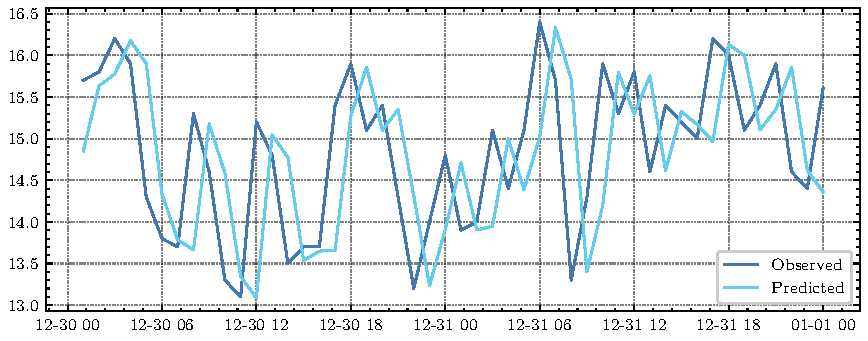
\includegraphics[width=\textwidth]{Wind Speed Prediction (Wavelet)}
  \caption{小波分解 ARIMA-SVR 組合模型短期風速預測結果}
  \label{figure: Wind Speed Prediction Wavelet}
\end{figure}

\subsection{模型誤差比較}

為比較在短期風速預測中採用小波分解 ARIMA-SVR 組合模型是否相較傳統單一預測模型具有較好的效果,本文中使用同一段時間內的歷史風速資料,分別採用了單一 ARIMA 預測模型、單一 SVR 預測模型、一般等權 ARIMA-SVR 組合模型與小波分解 ARIMA-SVR 組合模型進行預測。

計算其平均絕對百分比誤差(MAPE)、平均絕對誤差(MAE)與均方根誤差(RMSE)作為模型優劣的評價依據,結果如表 \ref{table: Time Series Model Result} 所示。

\begin{table}[htp]
  \centering
  \caption[風速預測模型評估結果]{風速預測模型評估結果}
  \begin{tabular}{lccc}
    \toprule
    \textbf{模型}               & \textbf{MAPE} & \textbf{MAE} & \textbf{RMSE} \\
    \midrule
    單一 ARIMA 預測模型         & $5.3022 \%$   & $0.7817$     & $0.9692$      \\
    單一 SVR 預測模型           & $5.4723 \%$   & $0.8113$     & $0.9869$      \\
    一般等權 ARIMA-SVR 組合模型 & $5.2852 \%$   & $0.7762$     & $0.9651$      \\
    小波分解 ARIMA-SVR 組合模型 & $5.1487 \%$   & $0.7319$     & $0.9517$      \\
    \bottomrule
  \end{tabular}
  \label{table: Time Series Model Result}
\end{table}

\section{收益結果分析}

\subsection{電動汽車有無影響}

比較同一風力電場在有電動汽車作為儲能設備參與虛擬電廠與沒有電動汽車作為儲能設備參與虛擬電廠的收益,使用模型預測控制方法進行求解。

將每個月份中,將整合了電動汽車作為儲能設備的虛擬電廠收益記為 $\text{Profit}_{\text{with EV}}(t)$,而未整合電動汽車作為儲能設備的虛擬電廠收益記為 $\text{Profit}_{\text{without EV}}(t)$,
則可以將整合了電動汽車作為儲能設備的虛擬電廠收益增長率表示如方程式 \eqref{equation: Profit Growth Rate} 所示。

\begin{equation}\label{equation: Profit Growth Rate}
  R_{\text{growth}} = \frac{\text{Profit}_{\text{with EV}}(t) - \text{Profit}_{\text{without EV}}(t)}{\text{Profit}_{\text{without EV}}(t)} \times 100 \%
\end{equation}

模擬結果顯示,整合了電動汽車作為儲能設備的虛擬電廠相較未整合電動汽車作為儲能設備的虛擬電廠,具有較高的收益。此外,當 $\sigma$ 值較小時,由於儲能成本較低,而使虛擬電廠在電力市場電價較低時,儘可能儲存電力並於電力市場電價較高時進行販售。

\subsection{電動汽車數量需求}

\section{小結}
% !TeX root = ../main.tex

\chapter{結論與建議}

\section{研究總結}

本研究以虛擬電廠 (Virtual Power Plant, VPP) 概念整合風力電場與電動汽車,透過預測風速配合風機功率模型取得風力機組發電數量後,考慮電動汽車作為儲能設備來參與電力市場交易,並透過模型預測控制 (Model Predictive Control, MPC) 在有限時域下針對動態變化的虛擬電廠進行儲能調度來獲得最佳收益。主要工作包括:

% \begin{enumerate}[label = (\arabic*)]
\begin{itemize}
  \item 提出使用小波轉換分解風速時間序列的 SVR-ARIMA 組合預測模型,用以提高收益模型中短期風速的預測能力,使其能更準確地估算風力發電數量。
  \item 以虛擬電廠概念整合風力電場與電動汽車作為儲能設備,建構其參與電力市場的收益模型。
  \item 採用模型預測控制方法,在有限時域下針對動態變化的虛擬電廠進行調度,根據結果進行收益分析與討論。
\end{itemize}

案例分析中,本研究採用我國\uline{澎湖}地區\uline{東吉島} (DONGJIDAO) 測站的歷史風速作為風速預測模型之驗證,並作為後續收益分析之依據。案例分析結果提供我們以下結論:

\begin{itemize}
  \item 短期風速預測中,採用小波分解 ARIMA-SVR 組合預測模型,透過平均絕對誤差 (Mean Absolute Error, MAE) 和均方根誤差 (Root Mean Squares Error, RMSE) 進行預測能力評價,顯示相較於單一 ARIMA 預測模型或單一 SVR 預測模型能提高預測能力。
  \item 整合電動汽車作為儲能設備,相較於沒有使用電動汽車作為儲能設備的虛擬電廠有著更高的收益;在本研究所模擬的情境下,最高能有 $15.41\%$ 的收益成長。
  \item 本文所建構之模型可用於估算虛擬電廠最佳收益,以及為達最佳收益所需的電動汽車數量。在本研究所模擬的情境下,假設電動車電池放電深度為 $\text{DoD}=0.25$ 時,電動汽車數量需求範圍約在 $1,721$ 輛至 $5,651$ 輛之間。
\end{itemize}

\section{研究限制}

受限於實務上的困難,本研究仍有一些不足之處。以下補充說明本研究存在的限制條件以及未來可以改善的方向:

\begin{enumerate}[label = (\arabic*)]
  \item 案例分析中作為短期風速預測依據的觀測風速採用氣象測站資料,與實際風場內的風速之間存在差異,無法真實反映場址的預測發電數量;若能取得並參考場址內的歷史風速資料,應能更準確地預測風力發電數量。
  \item 受限於氣象資料的觀測時間,本研究中採用一小時作為調度間隔,無法兼顧因再生能源的發電數量在短時間內有劇烈變化的情境;未來可以根據資料狀況縮小調度的時間間隔,然而對於計算設備規格要求較高,且電動汽車行為較不容易於短時間內進行控制。
  \item 研究中假設虛擬電廠中的電動汽車在時段內的行為是可以被控制的,但真實世界中每位車主的行為有太多變數存在;盼未來能有更佳的方法對這部分進行量化分析。
  \item 研究中假設虛擬電廠在販售電力資源至電力市場時不需要考慮市場需求,但真實世界中可能會遭遇特定季節或時段出現電力過剩的狀況。
  \item 科技日新月異加上政策並非一成不變,比如案例分析中所使用的電動汽車與時間電價數據,可能在未來有大幅度的變動,本文結論亦需進行滾動式修正。
\end{enumerate}

欲以有限的模型描述現實中萬千的變化幾乎無法做到,因此本研究上仍有許多限制與改善之處無法一一陳列,僅期望透過有限的資料在所能描述的範疇內儘可能地表達看法。

% \section{結語}

% 能源議題不僅與

% 參考文獻
% References
\refmatter
\bibliographystyle{IEEEtran}
\bibliography{back/references}


% 附錄
% Appendices
% !TeX root = ../main.tex

\appendix{A}{再生能源場址}

% https://tw.datagove.com/opendata.aspx?sn=105909713
下述資料為臺灣電力公司所開放之我國再生能源場址資料,包含了我國再生能源各場址名稱、製造商、機組型號、單機運轉容量、安全調度日(與電力系統進行併聯後,發電時數長達 $96$ 小時以上之初始調度日)、地址與座標。

% 臺灣風力發電場址資料
\begin{landscape}
\begin{table}[htp]
  \centering
  \caption[臺灣風力發電場址資料]{臺灣風力發電場址資料}
  \begin{tabular}{lllrlll}
    \toprule
    \textbf{場址名稱(機組)} & \textbf{製造廠商/承包廠商} & \textbf{機組型號} & \textbf{運轉容量} & \textbf{安全調度日} & \textbf{地址} & \textbf{座標} \\
    & & & (\si{kW})& & & \\
    \midrule
    石門風力(\#1 - \#6) & 丹麥 Vestas(中興) & V47 & $660$ & $2004/10/01$ & 新北市石門區 & $25°17'34.6″N, 121°34'54.5″E$ \\
    林口風力(\#4 - \#6) & 丹麥 Vestas(星能) & V80 & $2000$ & $2010/09/08$ & 新北市林口區 & $25°07'22.9″N, 121°18'31.7″E$ \\
    蘆竹風力(\#1 - \#8) & 德國 ENERCON(中興)  & E44 & $900$ & $2014/10/31$ & 桃園市蘆竹區 & $25°07'03.4″N, 121°16'35.7″E$ \\
    觀園風力(\#1 - \#20) & 美國 GE(中興) & GE 1.5se & $1500$ & $2005/10/03$ & 桃園市觀音區 & $25°04'15.9″N, 121°07'09.6″E$ \\
    大潭風力(\#1 - \#3) & 美國 GE(中興) & GE 1.5se & $1500$ & $2005/03/18$ & 桃園市觀音區 & $25°01'17.4″N, 121°02'45.2″E$ \\
    大潭風力(\#4, \#5, \#8) & 丹麥 Vestas(星能) & V80 & $2000$ & $2011/02/07$ & 桃園市觀音區 & $25°01'33.1″N, 121°02'23.8″E$ \\
    大潭風力(\#6, \#7) & 德國 ENERCON(中興) & E70 & $2300$ & $2010/12/15$ & 桃園市觀音區 & $25°01'25.4″N, 121°02'24.4″E$ \\
    香山風力(\#1 - \#6) & 西班牙 Gamesa(漢翔) & Gamesa & $2000$ & $2008/10/30$ & 新竹市香山區 & $24°45'41.7″N, 120°54'16.9″E$ \\
    & & & & & & $24°44'45.0″N, 120°53'57.1″E$ \\
    中港風力(\#1 - \#18) & 荷蘭 Zephyros(樂士) & Zephyros Z-72 & $2000$ & $2008/07/19$ & 臺中市清水區 & $24°18'15.8″N, 120°32'40.4″E$ \\
    中火風力(\#2 - \#4) & 荷蘭 Zephyros(樂士) & Zephyros Z-72 & $2000$ & $2006/06/01$ & 臺中市龍井區 & $24°13'20.5″N, 120°28'39.8″E$ \\
    彰工風力(\#1 - \#23) & 丹麥 Vestas(星能) & V80 & $2000$ & $2006/12/05$ & 彰化縣伸港鄉 & $24°09'29.1″N, 120°27'20.8″E$ \\
    彰工風力(\#24 - \#31) & 丹麥 Vestas(星能) & V80 & $2000$ & $2010/11/16$ & 彰化縣伸港鄉 & $24°09'27.9″N, 120°25'46.2″E$ \\
    王功風力(\#1 - \#10) & 德國 ENERCON(中興) & E70 & $2300$ & $2010/11/15$ & 彰化縣芳苑鄉 & $23°59'21.4″N, 120°19'55.6″E$ \\
    麥寮風力(\#1 - \#15) & 丹麥 Vestas(漢翔) & V80 & $2000$ & $2008/12/16$ & 雲林縣麥寮鄉 & $23°49'12.0″N, 120°14'31.1″E$ \\
    麥寮風力(\#16 - \#23) & 丹麥 Vestas(星能) & V80 & $2000$ & $2009/12/27$ & 雲林縣麥寮鄉 & $23°48'39.5″N, 120°15'42.5″E$ \\
    四湖風力(\#1 - \#14) & 丹麥 Vestas(星能) & V80 & $2000$ & $2010/05/14$ & 雲林縣四湖鄉 & $23°39'11.1″N, 120°09'02.0″E$ \\
    \bottomrule
  \end{tabular}
  \label{table: Taiwan Wind Farm Data}
\end{table}
\end{landscape}

\begin{landscape}
\begin{table}[htp]
  \centering
  \begin{tabular}{lllrlll}
    \toprule
    \textbf{場址名稱(機組)} & \textbf{製造廠商/承包廠商} & \textbf{機組型號} & \textbf{運轉容量} & \textbf{安全調度日} & \textbf{地址} & \textbf{座標} \\
    & & & (\si{kW}) & & & \\
    \midrule
    恆春風力(\#1 - \#3) & 美國 GE(中興) & GE 1.5se & $1500$ & $2005/01/13$ & 屏東縣恆春鎮 & $21°57'18.4″N, 120°44'37.0″E$ \\
    中屯風力(\#1 - \#4) & 德國 ENERCON(中興) & E-40/6.44 & $600$ & $2001/09/13$ & 澎湖縣白沙鄉 & $23°37'12.9″N, 119°36'34.6″E$ \\
    中屯風力(\#5 - \#8) & 德國 ENERCON(中興) & E-40/6.44 & $600$ & $2005/06/30$ & 澎湖縣白沙鄉 & $23°36'57.0″N, 119°36'46.6″E$ \\
    湖西風力(\#1 - \#6) & 德國 ENERCON(中興) & E44 & $900$ & $2010/09/30$ & 澎湖縣湖西鄉 & $23°35'09.1″N, 119°40'40.1″E$ \\
    金沙風力(\#1 - \#2) & 丹麥 Vestas(星能) & V80 & $2000$ & $2009/11/28$ & 金門縣金沙鎮 & $24°29'20.2″N, 118°27'03.1″E$ \\
    \bottomrule
  \end{tabular}
\end{table}
\end{landscape}

% 臺灣太陽光電場址資料
\begin{landscape}
\begin{table}[htp]
  \centering
  \caption[臺灣太陽光電場址資料]{臺灣太陽光電場址資料}
  \begin{tabular}{lllrlll}
    \toprule
    \textbf{場址名稱(機組)} & \textbf{製造廠商/承包廠商} & \textbf{機組型號} & \textbf{運轉容量} & \textbf{安全調度日} & \textbf{地址} & \textbf{座標} \\
    & & & (\si{kW}) & & & \\
    \midrule
    大潭光電 & 亞力電機 & a2peak PEAK ON P230-60 & $235$ & $2012/07/28$ & 桃園市觀音區 & $25°01'52.3″N, 121°03'08.3″E$ \\
    中大光電 & 均豪精密 & AUO PM220P00 & $230$ & $2012/08/07$ & 桃園市中壢區 & $24°58'18.7″N, 121°12'02.0″E$ \\
    中部儲運光電 & 淳宇科技 & Apollo KAP-200-54 & $200$ & $2011/03/14$ & 臺中市后里區 & $24°19'22.5″N, 120°43'33.9″E$ \\
    新伯公光電 & 淳宇科技 & Sun Wall WD-A-CC-0872 & $85$ & $2011/03/14$ & 臺中市東勢區 & $24°13'16.9″N, 120°50'32.8″E$ \\
    卓蘭光電 & 均豪精密 & AUO PM220P00 & $230$ & $2011/09/18$ & 苗栗縣卓蘭鎮 & $24°19'11.3″N, 120°49'24.6″E$ \\
    & & SUNNER SOLAR SA-100 & $100$ & & \\
    台中電廠光電 & 台達電 & Kyocera KD210GH-2P & $210$ & $2010/02/07$ & 臺中市龍井區 & $24°12'29.2″N, 120°29'28.9″E$ \\
    ( D, E 生水池) & & & & & \\
    台中電廠光電 & 華城電機 & Delsolar D6p240B3A & $240$ & $2013/11/23$ & 臺中市龍井區 & $24°12'45.7″N, 120°29'26.9″E$ \\
    ( B, C 生水池) & & & & & \\
    龍井光電 & 互立機電 & TS-M240A3-6100 & $240$ & $2013/05/01$ & 臺中市龍井區 & $24°12'22.0″N, 120°29'43.0″E$ \\
    (一期 I 標) & & & & & \\
    龍井光電 & 華城電機 & Delsolar D6p240B3A & $240$ & $2013/01/30$ & 臺中市龍井區 & $24°12'32.6″N, 120°29'37.4″E$ \\
    (一期 II 標) & & & & & \\
    龍井光電 & 亞力電機 & GreenTriplex PM245P00 & $255$ & $2014/08/06$ & 臺中市龍井區 & $24°12'31.0″N, 120°29'43.6″E$ \\
    (二期) & & & & & \\
    \bottomrule
  \end{tabular}
  \label{table: Taiwan Solar Data}
\end{table}
\end{landscape}

\begin{landscape}
\begin{table}[htp]
  \centering
  \begin{tabular}{lllrlll}
    \toprule
    \textbf{場址名稱(機組)} & \textbf{製造廠商/承包廠商} & \textbf{機組型號} & \textbf{運轉容量} & \textbf{安全調度日} & \textbf{地址} & \textbf{座標} \\
    & & & (\si{kW}) & & & \\
    \midrule
    后里光電 & 大同公司 & ASEC-245G6M & $225$ & $2012/10/06$ & 臺中市后里區 & $24°19'05.3″N, 120°44'23.0″E$ \\
    民雄光電 & 淳宇科技 & SuN Wall WD-A-CC-0872 & $85$ & $2011/03/14$ & 嘉義縣民雄鄉 & $23°31'29.0″N, 120°27'22.9″E$ \\
    永安鹽灘光電 & 華城電機 & SUNTECH STP280-24/vd & $280$ & $2011/12/29$ & 高雄市永安區 & $22°50'12.6″N, 120°12'23.5″E$ \\
    興達電廠光電 & 茂迪光電 & Kyocera KD210GH-2P & $210$ & $2010/06/01$ & 高雄市茄萣區 & $22°51'11.5″N, 120°12'03.2″E$ \\
    ( \#3 - \#6 生水池) & & & & & \\
    興達電廠光電 & 均豪精密 & AUO PM220P00 & $230$ & $2010/09/18$ & 高雄市茄萣區 & $22°51'11.5″N, 120°12'03.2″E$ \\
    ( SCR 生水池) & & & & & \\
    興達電廠光電 & 華城電機 & Delsolar D6p240B3A & $240$ & $2013/11/23$ & 高雄市茄萣區 & $22°51'11.5″N, 120°12'03.2″E$ \\
    ( \#1 - \#2 生水池) & & & & & \\
    路北光電 & 均豪精密 & AUO PM220P00 & $230$ & $2011/06/05$ & 高雄市鼓山區 & $22°50'17.2″N, 120°14'52.6″E$ \\
    核三廠光電 & 益鼎工程 & SUNTECH STP280-24/vd & $280$ & $2012/07/20$ & 屏東縣恆春鎮 & $21°57'21.1″N, 120°44'25.5″E$ \\
    澎湖光電 & 均豪精密 & AUO PM220P00 & $230$ & $2011/05/10$ & 澎湖縣湖西鄉 & $23°33'50.7″N, 119°39'32.5″E$ \\
    金門光電 & 錦億實業 & Apollo KAP-200 & $200$ & $2010/03/14$ & 金門縣金沙鎮 & $24°29'49.0″N, 118°24'09.8″E$ \\
    七美光電 & 廣運機械 & KENMEC TKSA-23001 & $230$ & $2012/03/08$ & 澎湖縣七美鄉 & $23°12'15.3″N, 119°26'29.6″E$ \\
    (一期) & & & & & \\
    七美光電 & 大同電機 & GTEC295G6S6A & $295$ & $2018/01/22$ & 澎湖縣七美鄉 & $23°12'15.3″N, 119°26'29.6″E$ \\
    (二期) & & & & & \\
    \bottomrule
  \end{tabular}
\end{table}
\end{landscape}

\begin{landscape}
\begin{table}[htp]
  \centering
  \begin{tabular}{lllrlll}
    \toprule
    \textbf{場址名稱(機組)} & \textbf{製造廠商/承包廠商} & \textbf{機組型號} & \textbf{運轉容量} & \textbf{安全調度日} & \textbf{地址} & \textbf{座標} \\
    & & & (\si{kW}) & & & \\
    \midrule
    龍潭光電 & 太創能源 & MM60 SRT 300 & $300$ & $2018/01/04$ & 桃園市龍潭區 & $24°49'11.1″N, 121°11'37.8″E$ \\
    竹工光電 & 太創能源 & MM60 SRT 300 & $300$ & $2018/02/09$ & 新竹縣湖口鄉 & $24°53'35.7″N, 121°05'37.2″E$ \\
    中科光電 & 太創能源 & MM60 SRT 300 & $300$ & $2018/03/30$ & 台中市西屯區 & $24°12'04.1″N, 120°36'26.8″E$ \\
    彰林光電 & 太創能源 & MM60 SRT 300 & $300$ & $2018/04/25$ & 彰化縣埤頭鄉 & $23°55'44.4″N, 120°27'21.4″E$ \\
    台南七股光電 & 華城電機 & D6M-305-E3A & $305$ & $2018/09/12$ & 台南市七股區 & $23°05'47.1″N, 120°08'09.0″E$ \\
    高雄ES光電 & 立碁電子 & GTEC 295G6S6A & $295$ & $2018/05/22$ & 高雄市三民區 & $22°38'46.6″N, 120°17'38.2″E$ \\
    燕巢光電 & 立碁電子 & GTEC 295G6S6A & $295$ & $2018/05/31$ & 高雄市燕巢區 & $22°46'28.8″N, 120°23'11.0″E$ \\
    大潭光電 & 富台工程 & D6M305H3A & $305$ & $2018/11/01$ & 桃園市觀音區 & $25°01'21.9″N, 121°02'51.9″E$ \\
    北儲光電 & 富台工程 & D6M305H3A & $305$ & $2018/11/26$ & 桃園市觀音區 & $25°01'35.0″N, 121°03'36.8″E$ \\
    彰濱光電 & 中華電信 & D6L295K3A & $295$ & $2019/02/18$ & 彰化縣鹿港鎮 & $24°06'26.6″N, 120°23'46.0″E$ \\
    \bottomrule
  \end{tabular}
\end{table}
\end{landscape}
% !TeX root = ../main.tex

\appendix{B}{風力機組規格}

本文研究的案例分析中,採用\uline{澎湖}地區作為示範,根據表 \ref{table: Taiwan Wind Farm Data} 的我國風力發電場址資料所示,該地區設有 Enercon E40/600 Model 與 Enercon E44/900 Model 風力機組,下述為此二風力機組之規格資料。

\section{Enercon E40/600 Model}

\subsection*{風機規格資料}

\begin{itemize}
  \item 額定功率 (Rated Power) :$600$ \si{\kW}
  \item 轉子直徑 (Rotor Diameter) :$40$ \si{\meter}
  \item 掃掠面積 (Swept Area) :$1,257$ \si{\meter\squared}
  \item 能量密度 (Power Density) :$2.1$ \si{\meter\squared}/\si{\kW}
  \item 葉片數量 (Number of Blades) :$3$ 片
  \item 葉輪最小額定轉速 (Minimum Rotor Speed) :$18$ \si{rd}/\si{\min}
  \item 葉輪最大額定轉速 (Maximum Rotor Speed) :$34.5$ \si{rd}/\si{\min}
  \item 額定風速 (Rated Wind Speed) :$13$ \si{m}/\si{s}
  \item 切入風速 (Cut-in Wind Speed) :$2.5$ \si{m}/\si{s}
  \item 切出風速 (Cut-off Wind Speed) :$25$ \si{m}/\si{s}
\end{itemize}

\subsection*{風機功率曲線}

\begin{figure}[htbp]
  \centering
  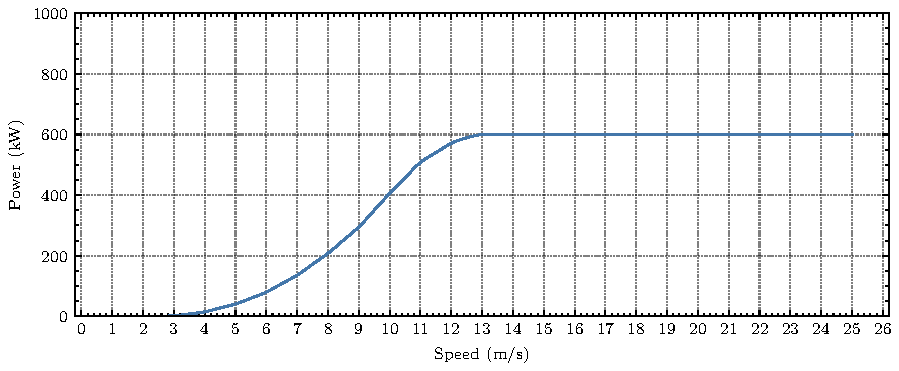
\includegraphics[width=\textwidth]{Enercon E40 600 Model}
  \caption{Enercon E40/600 Model 風機功率曲線}
  \label{figure: Enercon E40/600 Model}
\end{figure}

\section{Enercon E44/900 Model}

\subsection*{風機規格資料}

\begin{itemize}
  \item 額定功率 (Rated Power) :$900$ \si{\kW}
  \item 轉子直徑 (Rotor Diameter) :$44$ \si{\meter}
  \item 掃掠面積 (Swept Area) :$1521$ \si{\meter\squared}
  \item 葉片數量 (Number of Blades) :$3$ 片
  \item 葉輪最小額定轉速 (Minimum Rotor Speed) :$16$ \si{rd}/\si{\min}
  \item 葉輪最大額定轉速 (Maximum Rotor Speed) :$34.5$ \si{rd}/\si{\min}
  \item 額定風速 (Rated Wind Speed) :$17$ \si{m}/\si{s}
  \item 切入風速 (Cut-in Wind Speed) :$3$ \si{m}/\si{s}
  \item 切出風速 (Cut-off Wind Speed) :$25$ \si{m}/\si{s}
\end{itemize}

\subsection*{風機功率曲線}

\begin{figure}[htbp]
  \centering
  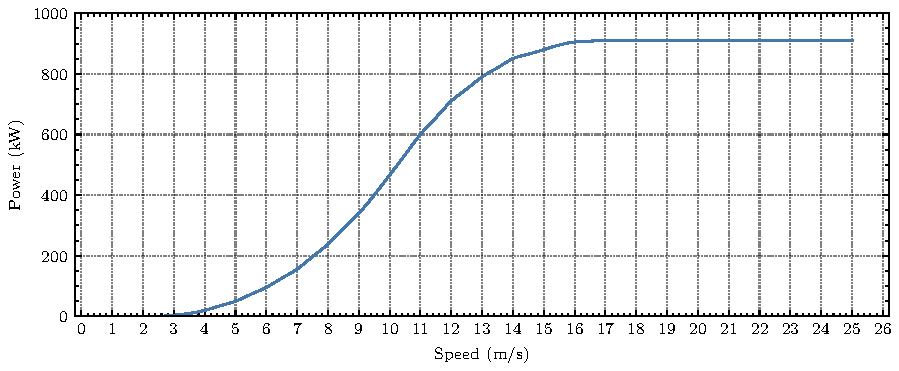
\includegraphics[width=\textwidth]{Enercon E44 900 Model}
  \caption{Enercon E44/900 Model 風機功率曲線}
  \label{figure: Enercon E44/900 Model}
\end{figure}


\end{document}
